% A LaTeX template for MSc Thesis submissions to 
% Politecnico di Milano (PoliMi) - School of Industrial and Information Engineering
%
% S. Bonetti, A. Gruttadauria, G. Mescolini, A. Zingaro
% e-mail: template-tesi-ingind@polimi.it
%
% Last Revision: October 2021
%
% Copyright 2021 Politecnico di Milano, Italy. NC-BY

\documentclass{Configuration_Files/PoliMi3i_thesis}

%------------------------------------------------------------------------------
%	REQUIRED PACKAGES AND  CONFIGURATIONS
%------------------------------------------------------------------------------

% CONFIGURATIONS
\usepackage{parskip} % For paragraph layout
\usepackage{setspace} % For using single or double spacing
\usepackage{emptypage} % To insert empty pages
\usepackage{multicol} % To write in multiple columns (executive summary)
\setlength\columnsep{15pt} % Column separation in executive summary
\setlength\parindent{0pt} % Indentation
\raggedbottom  

\setcounter{tocdepth}{3}
\setcounter{secnumdepth}{3}


% PACKAGES FOR TITLES
\usepackage{titlesec}
% \titlespacing{\section}{left spacing}{before spacing}{after spacing}
\titlespacing{\section}{0pt}{3.3ex}{2ex}
\titlespacing{\subsection}{0pt}{3.3ex}{1.65ex}
\titlespacing{\subsubsection}{0pt}{3.3ex}{1ex}
\usepackage{color}

% PACKAGES FOR LANGUAGE AND FONT
\usepackage[english]{babel} % The document is in English  
\usepackage[utf8]{inputenc} % UTF8 encoding
\usepackage[T1]{fontenc} % Font encoding
\usepackage[11pt]{moresize} % Big fonts

% PACKAGES FOR IMAGES
\usepackage{graphicx}
\usepackage{transparent} % Enables transparent images
\usepackage{eso-pic} % For the background picture on the title page
\usepackage{subfig} % Numbered and caption subfigures using \subfloat.
\usepackage{tikz} % A package for high-quality hand-made figures.
\usetikzlibrary{}
\graphicspath{{./Images/}} % Directory of the images
\usepackage{caption} % Coloured captions
\usepackage{xcolor} % Coloured captions
\usepackage{amsthm,thmtools,xcolor} % Coloured "Theorem"
\usepackage{float}

% STANDARD MATH PACKAGES
\usepackage{amsmath}
\usepackage{amsthm}
\usepackage{amssymb}
\usepackage{amsfonts}
\usepackage{bm}
\usepackage[overload]{empheq} % For braced-style systems of equations.
\usepackage{fix-cm} % To override original LaTeX restrictions on sizes

% PACKAGES FOR TABLES
\usepackage{tabularx}
\usepackage{longtable} % Tables that can span several pages
\usepackage{colortbl}

% PACKAGES FOR ALGORITHMS (PSEUDO-CODE)
\usepackage{algorithm}
\usepackage{algorithmic}

% PACKAGES FOR REFERENCES & BIBLIOGRAPHY
\usepackage[colorlinks=true,linkcolor=black,anchorcolor=black,citecolor=black,filecolor=black,menucolor=black,runcolor=black,urlcolor=black]{hyperref} % Adds clickable links at references
\usepackage{cleveref}
\usepackage[square, numbers, sort&compress]{natbib} % Square brackets, citing references with numbers, citations sorted by appearance in the text and compressed
\bibliographystyle{abbrvnat} % You may use a different style adapted to your field

% OTHER PACKAGES
\usepackage{pdfpages} % To include a pdf file
\usepackage{afterpage}
\usepackage{lipsum} % DUMMY PACKAGE
\usepackage{fancyhdr} % For the headers
\fancyhf{}

%ADDED PACKAGES BY DAVIDE
\usepackage{caption} 
\usepackage{mhchem}
%\captionsetup[figure]{skip=-25pt}
\newcommand{\mycomment}[1]{}

% Input of configuration file. Do not change config.tex file unless you really know what you are doing. 
% Define blue color typical of polimi
\definecolor{bluepoli}{cmyk}{0.4,0.1,0,0.4}

% Custom theorem environments
\declaretheoremstyle[
  headfont=\color{bluepoli}\normalfont\bfseries,
  bodyfont=\color{black}\normalfont\itshape,
]{colored}

% Set-up caption colors
\captionsetup[figure]{labelfont={color=bluepoli}} % Set colour of the captions
\captionsetup[table]{labelfont={color=bluepoli}} % Set colour of the captions
\captionsetup[algorithm]{labelfont={color=bluepoli}} % Set colour of the captions

\theoremstyle{colored}
\newtheorem{theorem}{Theorem}[chapter]
\newtheorem{proposition}{Proposition}[chapter]

% Enhances the features of the standard "table" and "tabular" environments.
\newcommand\T{\rule{0pt}{2.6ex}}
\newcommand\B{\rule[-1.2ex]{0pt}{0pt}}

% Pseudo-code algorithm descriptions.
\newcounter{algsubstate}
\renewcommand{\thealgsubstate}{\alph{algsubstate}}
\newenvironment{algsubstates}
  {\setcounter{algsubstate}{0}%
   \renewcommand{\STATE}{%
     \stepcounter{algsubstate}%
     \Statex {\small\thealgsubstate:}\space}}
  {}

% New font size
\newcommand\numfontsize{\@setfontsize\Huge{200}{60}}

% Title format: chapter
\titleformat{\chapter}[hang]{
\fontsize{50}{20}\selectfont\bfseries\filright}{\textcolor{bluepoli} \thechapter\hsp\hspace{2mm}\textcolor{bluepoli}{|   }\hsp}{0pt}{\huge\bfseries \textcolor{bluepoli}
}

% Title format: section
\titleformat{\section}
{\color{bluepoli}\normalfont\Large\bfseries}
{\color{bluepoli}\thesection.}{1em}{}

% Title format: subsection
\titleformat{\subsection}
{\color{bluepoli}\normalfont\large\bfseries}
{\color{bluepoli}\thesubsection.}{1em}{}

% Title format: subsubsection
\titleformat{\subsubsection}
{\color{bluepoli}\normalfont\large\bfseries}
{\color{bluepoli}\thesubsubsection.}{1em}{}

% Shortening for setting no horizontal-spacing
\newcommand{\hsp}{\hspace{0pt}}

\makeatletter
% Renewcommand: cleardoublepage including the background pic
\renewcommand*\cleardoublepage{%
  \clearpage\if@twoside\ifodd\c@page\else
  \null
  \AddToShipoutPicture*{\BackgroundPic}
  \thispagestyle{empty}%
  \newpage
  \if@twocolumn\hbox{}\newpage\fi\fi\fi}
\makeatother

%For correctly numbering algorithms
\numberwithin{algorithm}{chapter}

%----------------------------------------------------------------------------
%	NEW COMMANDS DEFINED
%----------------------------------------------------------------------------

% EXAMPLES OF NEW COMMANDS
\newcommand{\bea}{\begin{eqnarray}} % Shortcut for equation arrays
\newcommand{\eea}{\end{eqnarray}}
\newcommand{\e}[1]{\times 10^{#1}}  % Powers of 10 notation

%----------------------------------------------------------------------------
%	ADD YOUR PACKAGES (be careful of package interaction)
%----------------------------------------------------------------------------

%----------------------------------------------------------------------------
%	ADD YOUR DEFINITIONS AND COMMANDS (be careful of existing commands)
%----------------------------------------------------------------------------

%----------------------------------------------------------------------------
%	BEGIN OF YOUR DOCUMENT
%----------------------------------------------------------------------------

\begin{document}

\fancypagestyle{plain}{%
\fancyhf{} % Clear all header and footer fields
\fancyhead[RO,RE]{\thepage} %RO=right odd, RE=right even
\renewcommand{\headrulewidth}{0pt}
\renewcommand{\footrulewidth}{0pt}}

%----------------------------------------------------------------------------
%	TITLE PAGE
%----------------------------------------------------------------------------

\pagestyle{empty} % No page numbers
\frontmatter % Use roman page numbering style (i, ii, iii, iv...) for the preamble pages

\puttitle{
	title = Use of Laser Induced Breakdown Spectroscopy to investigate the chemical composition of glass surfaces after optics manufacturing, % Title of the thesis
	name = {Davide Notaro, Emanuele Locati}, %\and Davide Notaro, % Author Name and Surname
	course = Engineering Physics - Ingegneria Fisica, % Study Programme (in Italian)
	ID = {103558, 103577},  % Student ID number (numero di matricola)
    coadvisor=, % Co-Supervisor name, remove this line if there is none
	advisor = Prof. Christoph Gerhard, % Supervisor name
	academicyear = {2023-2024},  % Academic Year
} % These info will be put into your Title page 

	
%----------------------------------------------------------------------------
%	PREAMBLE PAGES: ABSTRACT (inglese e italiano), EXECUTIVE SUMMARY
%----------------------------------------------------------------------------
\startpreamble
\setcounter{page}{1} % Set page counter to 1

% ABSTRACT IN ENGLISH
\chapter*{Abstract} 
Laser Induced Breakdown Spectroscopy (LIBS) is an experimental technique for elemental analysis based on the atomic emission of a plasma generated by a high-energy laser pulse. The aim of this work is to use the aforementioned technique to investigate the presence of impurities resulting from the grinding and polishing process in samples of optical glass. These impurities may originate from minerals dissolved in the water used or from chemical species in the polishing agent. Specifically, the study examines whether the diffusion process is the main cause of this phenomenon, with a focus on the temporal dependence of contaminants concentration.
\\
The introductory chapters provide an overview of the experimental techniques used, the theory underlying glass polishing, and the selection of variables under investigation. Theoretical predictions based on Fick's diffusion theory are also presented.
\\
The final section is dedicated to the presentation and analysis of the measurements taken, along with an exploration of potential reasons why these measurements may not align with the proposed hypotheses.
\\
Additionally, the study investigates whether the use of distilled water throughout various stages of the process could influence the purity of the final glass product.
\\
\\
\textbf{Keywords:} LIBS, optical glass, chemical mechanical polishing, diffusion, contamination analysis % Keywords
% ABSTRACT IN ITALIAN
\chapter*{Sommario}
Laser Induced Breakdown Spectroscopy (LIBS) è una tecnica sperimentale di analisi elementale basata sull'emissione atomica di un plasma generato da un impulso laser ad alta energia. L'obiettivo di questo lavoro è utilizzare la tecnica sopracitata per indagare sulla presenza di impurità dovute al processo di smerigliatura e lucidatura in campioni di vetro ottico, provenienti sia dai minerali disciolti nell'acqua utilizzata sia dalle specie chimiche facenti parte dell'agente lucidante.  In particolare, verificando se il processo di diffusione sia la principale causa di questo fenomeno, prestando attenzione alla dipendenza temporale della concentrazione dei contaminanti.
\\
Nei primi capitoli è presente un'introduzione sulle tecniche sperimentali utilizzate, sulla teoria alla base della rifinitura del vetro e sulla scelta delle variabili investigate. Sono anche presenti predizioni teoriche dei possibili risultati, basate sulla teoria della diffusione di Fick. 
\\
La parte finale è invece dedicata alla presentazione e all'analisi delle misurazioni effettuate, e alle possibili cause del perché queste non rispecchiano le ipotesi proposte.  
\\
In aggiunta, viene verificato se l'utilizzo di acqua distillata durante tutte le diverse fasi del processo può avere un'influenza sulla purezza del vetro finale.
\\
\\
\textbf{Parole chiave:} LIBS, vetro ottico, lucidatura meccanica chimica, diffusione, analisi delle impurità % Keywords (italian)

%----------------------------------------------------------------------------
%	LIST OF CONTENTS/FIGURES/TABLES/SYMBOLS
%----------------------------------------------------------------------------

% TABLE OF CONTENTS
\thispagestyle{empty}
\tableofcontents % Table of contents 
\thispagestyle{empty}
\cleardoublepage

%-------------------------------------------------------------------------
%	THESIS MAIN TEXT
%-------------------------------------------------------------------------
% In the main text of your thesis you can write the chapters in two different ways:
%
%(1) As presented in this template you can write:
%    \chapter{Title of the chapter}
%    *body of the chapter*
%
%(2) You can write your chapter in a separated .tex file and then include it in the main file with the following command:
%    \chapter{Title of the chapter}
%    \input{chapter_file.tex}
%
% Especially for long thesis, we recommend you the second option.

\addtocontents{toc}{\vspace{2em}} % Add a gap in the Contents, for aesthetics
\mainmatter % Begin numeric (1,2,3...) page numbering

% --------------------------------------------------------------------------
% NUMBERED CHAPTERS % Regular chapters following
% --------------------------------------------------------------------------
\chapter*{Introduction}

Laser Induced Breakdown Spectroscopy (LIBS) is a powerful analytical method that allows for the detection of the elemental composition of a target sample. It is commended for its balance between precision, speed, and high sensitivity that permits to identify small traces of impurities. Beyond all of this, its high versatility made it a common choice for a plurality of applications.
\\
We employed a specific calibration-free approach of LIBS to investigate the presence of contaminants in optical glasses due to grinding and polishing. All the processes involved in chemical-mechanical polishing leave surface defects that can influence the optical properties of the material, it is of interest for the industry to study and describe the contamination process in order to understand its characteristics and minimize its effects.
\\
 A possible dependence on polishing time, polish concentration and type of water is going to be investigated.
 \\
 \\
In Chapter~\ref{ch:experimental_techniques} a thorough discussion on the experimental techniques is carried out.
\\
In Chapter~\ref{ch:glass_manufacturing} the theoretical description of the post-processes of glass manufacturing is presented, complete with the details on the grinding and polishing phases.
\\
The main premises, the objectives and the predictions of the research are introduced in Chapter~\ref{ch:research_premises}, while in Chapter~\ref{ch:experimental_setup} are described the experimental setup and the followed workflow for every technique employed, with a focus on the methods used to find the optimal parameters and the analysis of the measured data.
\\
Lastly, in Chapter~\ref{ch:experimental_results} are presented the results and their interpretation.



\chapter{Experimental Techniques}
\label{ch:experimental_techniques}

\section{LIBS}
\label{sec:LIBS}
Laser-Induced Breakdown Spectroscopy (LIBS) is an atomic emission spectroscopy technique that utilizes high energy laser pulses to create plasma on the surface of material samples. It is a promising method in analytical chemistry and material analysis because it allows for the direct analysis of solid, liquid and even gas samples, without requiring any chemical preparation.
\\
The interaction between focused laser pulses and the sample leads to the creation of a plasma composed of ionized matter. This plasma emission can yield spectral signatures indicative of the chemical composition of various materials, regardless of their state of matter [Source: Fundamentals and Applications].
\\
LIBS offers the capability of conducting both qualitative and accurate quantitative analyses. Qualitative analysis involves discriminating between different components of a target sample, whereas quantitative analysis goes further by not only identifying the chemical components but also determining their relative concentrations.
\\
However, due to the modest repeatability of the method, attributed to the high variability present between each experiment [Source: Applications of single-shot laser], LIBS does not enable researchers to achieve detection limits and precision as low as those attainable with other methods. Consequently, it is primarily utilized for qualitative, semi-quantitative, or comparative analysis.
\\
The promising performance of this spectroscopy technique as a quantitative chemical analysis system has been facilitated by the development of new spectral processing algorithms in the last decade. These advancements have significantly broadened the application fields of LIBS. Today, LIBS finds applications ranging from diagnostics of archaeological objects to remote material assessment in nuclear power plants, and from the analysis of metal diffusion in solar cells to geological analysis in space explorations.

\subsection{LIBS technique}
\label{subsec:LIBS_technique}
The processes involved in LIBS include laser-sample interaction, material removal, breakdown process, and element-specific emission.
\\
Initially, the interaction between focused laser pulses and the target sample leads to the vaporization of a specific part of the surface area as the temperature reaches the sample material’s boiling point. The evaporated material forms a plume above the sample surface, and due to the continuous energy absorption of the laser, can result in the generation of a high-temperature plasma that will expand and eventually cool down.
[Analytical Chemistry LIBS]

\begin{figure}[H]
    \centering
    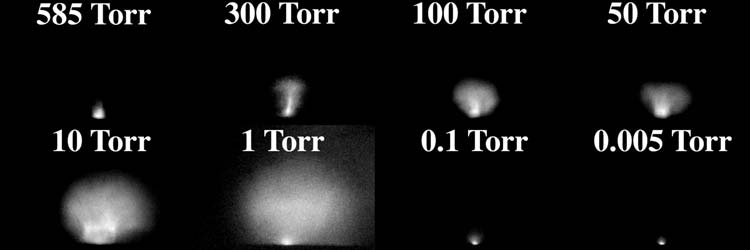
\includegraphics[width = 0.8\textwidth]{chapter_1/plasma_expansion_photo.png}
    \caption[Photo of a plasma expanding.]{ Change in the dimensions of a laser plasma as the air pressure was reduced.}
    \label{fig:plasma_expansion}
\end{figure}
[PHOTO TAKEN FROM LIBS: FUNDAMENTALS AND APPLICATIONS]

The light emitted from the plasma is indicative of the chemical composition of various materials. Positive identification of multiple elemental lines, including both wavelength and intensity within the emission spectrum, contributes to forming a unique spectral fingerprint of the target material. [Fundamentals and applications]
\\
The primary processes that occur during LIBS can be outlined in the following steps:

\begin{enumerate}
\item A short laser pulse is focused on the target material.
\item The incident optical energy is deposited on the sample, resulting in the vaporization of a small amount of its surface.
\item The incoming laser pulse, if its duration is sufficiently large, will also interact with the vapor plume to generate a high-temperature plasma.
\item The system employs a lens or an optical fiber to collect the light emitted from the plasma.
\item A dispersing device, such as a diffraction grating, spatially separates the emitted light into its components. This light originates from the spontaneous emission of hot atoms/ions in the plasma.
\item A digital sensor, such as a CCD or a PMT, is used to collect the light and generate the spectrum.
\item The wavelength and intensity of the resulting atomic emission peaks are analyzed to determine both the chemical elements present in the target sample and their relative concentrations.
\end{enumerate}
Each firing of the laser produces a single LIBS measurement. Typically, however, the signals from many laser plasmas are added or averaged to increase accuracy and precision and to average out nonconformities in sample composition. [LIBS Cambridge]

\begin{figure}[H]
    \centering
    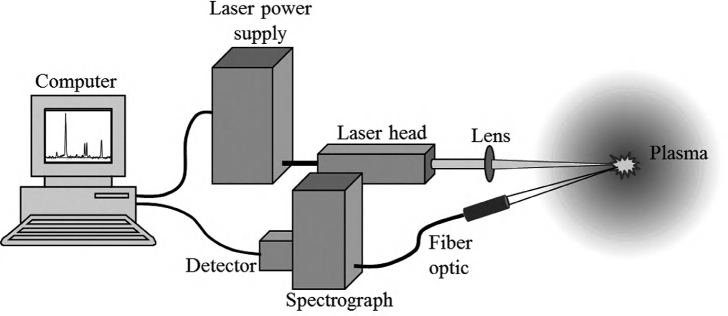
\includegraphics[width = \textwidth]{chapter_1/libs_setup.jpg}
    \caption{A schematic of a general apparatus for laser-induced breakdown spectroscopy illustrating the principal components.}
    \label{fig:libs_setup}
\end{figure}
[PHOTO TAKEN FROM HANDBOOK OF LIBS]

\subsection{Laser-sample Interaction}
\label{subsec:laser-sample_int}

When an atom absorbs a photon, it enters an excited state, where one of its electrons is promoted to a higher energy level. However, the excited states are not very stable, and electrons tend to transition to lower unpopulated energy levels either radiatively, when a photon is generated during the deexcitation process, and non-radiatively when the energy is dissipated in other forms, such as heat or vibration.
\\
Additionally, if the energy applied to the atom is sufficiently high to overcome the ionization potential, electrons can be detached from the atom, creating free negatively charged particles (electrons) and positively charged ions (cations). Initially, the outermost electron, with the lowest ionization potential, is the first to be detached. However, if the supplied energy is high enough, subsequent ionization potentials can be overcome, leading to the detachment of other electrons closer to the nucleus.
\\
There are two main steps leading to breakdown due to optical excitation. The first involves generating a few free electrons that serve as initial receptors of energy through collisions with photons and neutrals. The second is avalanche ionization in the focal region. Free electrons are accelerated by the electric field of the photons, and as the kinetic energy of the electrons grows, collisions will lead to further ionization that will generate even more electrons, creating an avalanche of ionization. 
\\
When a high-energy laser pulse is focused on the surface of a sample, if the irradiance at the focal point exceeds a certain threshold, atoms and ions are ejected from the surface in a process called ablation.

\begin{figure}[H]
    \centering
    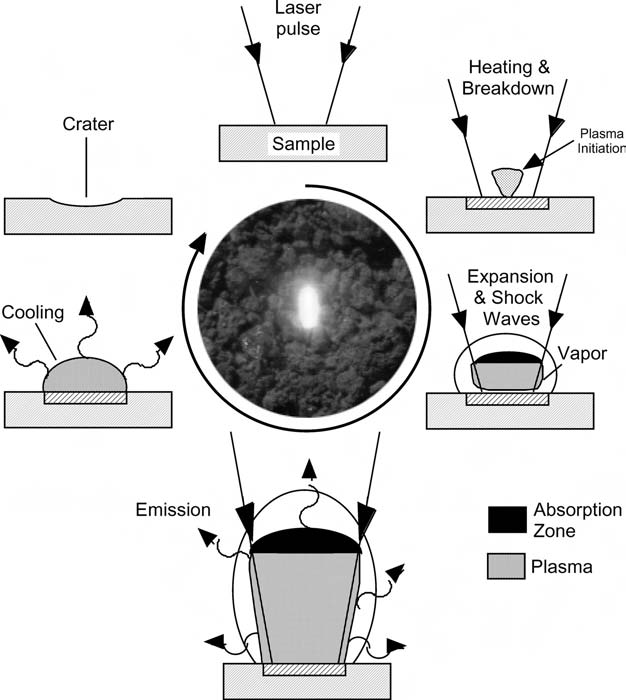
\includegraphics[width = 0.6\textwidth]{chapter_1/libs_life_cycle.png}
    \caption[LIBS life cycle.]{ Life cycle diagram showing main events in the LIBS process.}
    \label{fig:libs_life_cycle}
\end{figure}
[PHOTO TAKEN FROM Fundamentals and Applications]

\subsection{Plasma in LIBS}
\label{subsec:plasma_in_libs}
Given the numerous physical and chemical variables characterizing this state, various definitions of plasma are possible. A plasma can be defined as a local assembly of atoms, ions, molecules, and free electrons, that are overall electrically neutral and exhibit a collective behavior.
\\
Under typical conditions, such as atmospheric pressure and temperature, gases are primarily neutral, with only a marginable amount of charged particles. However, at high temperatures ($T > 1000K$), thermal dissociation of atoms and molecules occurs. Plasma forms when the average kinetic energy of the electrons (given by $k_bT$), significantly surpasses the average binding energy of an electron in an ion.
\\
Plasmas are characterized by a variety of parameters, such as the degree of ionization, the plasma temperature, and the electron density. Depending on the degree of ionization a plasma can be categorized as “weakly ionized”, where the ratio between electrons and other species is less than 10\%, or as “highly ionized” where, on the other hand, atoms could be stripped of many electrons, resulting in a very high electrons-to-ions ratio. LIBS plasmas typically fall in the first category of weakly ionized plasmas; in Figure~\ref{fig:plasma_parameters} we can see how LIBS plasmas compare in temperature and electron density relative to other types of plasma.
\begin{figure}[H]
    \centering
    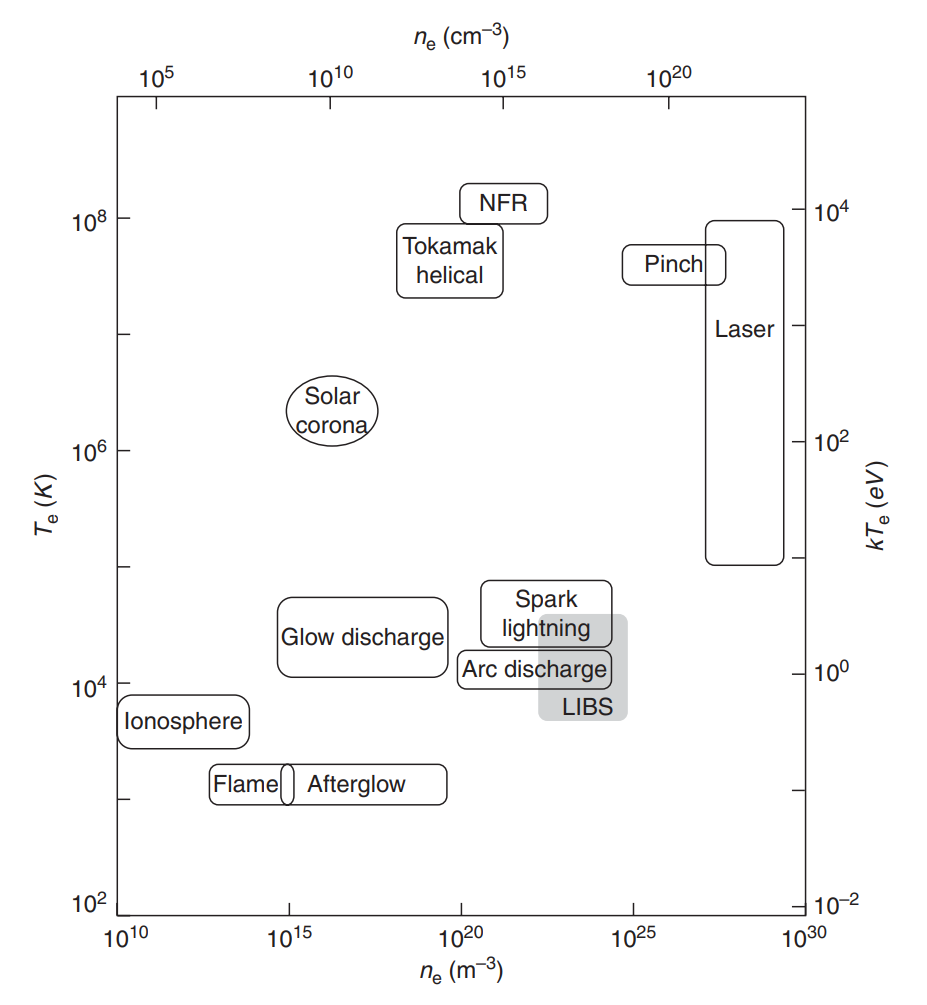
\includegraphics[width = 0.7\textwidth]{chapter_1/plasma_parameters.png}
    \caption{Relation between plasma parameters and type of plasma.}
    \label{fig:plasma_parameters}
\end{figure}
[PHOTO TAKEN FROM HANDBOOK OF LIBS]
The characteristics of the radiation emitted by the plasma depend on the type of radiative transitions that are occurring. At earlier times, where the plasma ionization level is high, the emission will be dominated by a continuum produced by both the bremsstrahlung (free-free transition) and the recombination processes (free-bound transition). Recombination occurs when a free electron is captured by a free ion, releasing its kinetic energy radiatively; while in bremsstrahlung the light is emitted due to electrons being accelerated or decelerated in collisions.
\\
However, the most interesting emissions that can be used for elemental analysis are caused by bound-to-bound transitions that occur between energy levels of ions, atoms, and molecules. 
\begin{figure}[H]
    \centering
    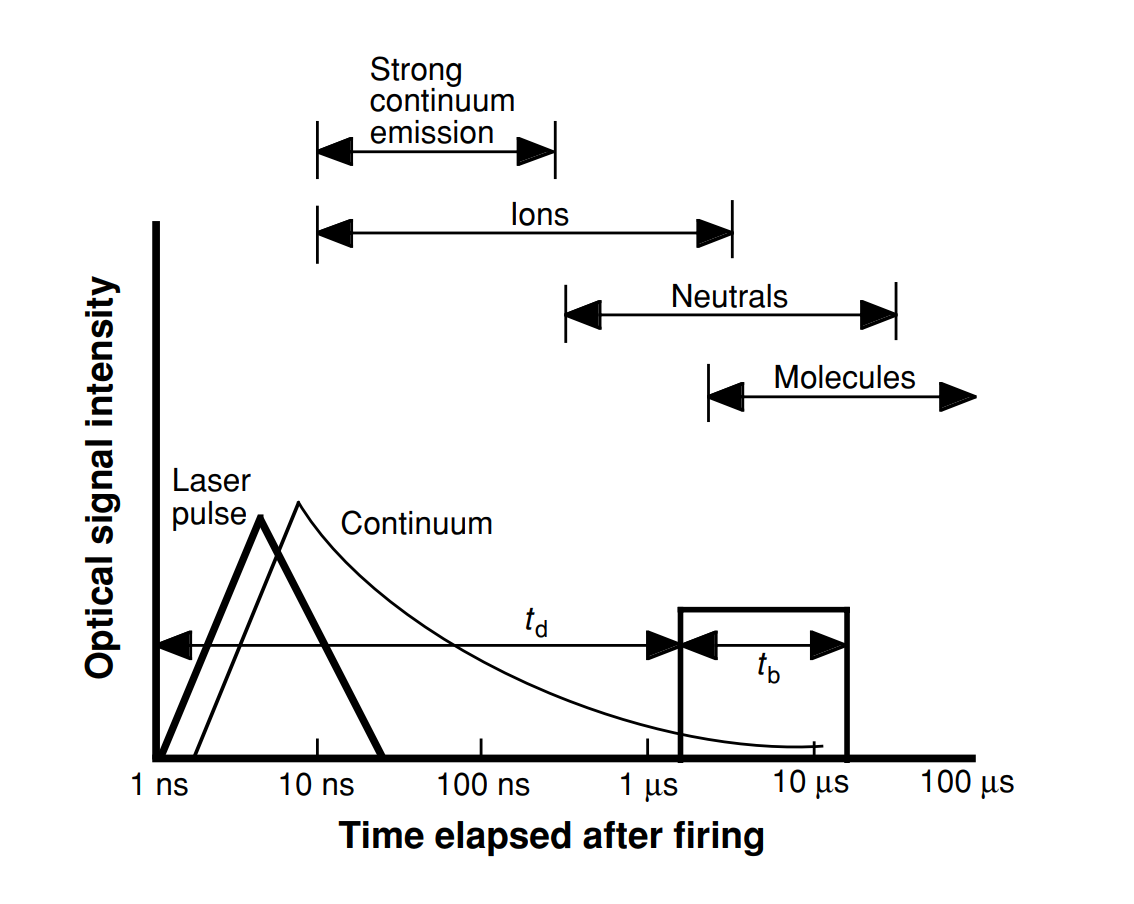
\includegraphics[width = \textwidth]{chapter_1/time_plasma_emission.png}
    \caption{Evolution of the emission of the LIBS plasma over time.}
    \label{fig:time_plasma_emission}
\end{figure}

\subsubsection{Plasma Parameters and Emission Characteristics}
\label{subsubsec:plasma_parameters}
Bound-to-bound transitions are characterized by a fixed energy value, equal to the energy difference between the initial and final level. However, experimentally we see that the measured emission spectrum is not constituted by a collection of sharp lines, but of bell curves instead, with different FWHM. This is because spectral line profiles are also influenced by broadening mechanisms; specifically, pure Doppler broadening, caused by the thermal movement of the emitting particles, will lead to a Gaussian profile, while natural line broadening, due to the time-energy uncertainty principle, and collision broadening will lead to a Lorentzian profile. The collisions between ions and electrons will result in Stark broadening due to the presence of high intensity electric fields near the particles; this phenomenon is predominant in plasmas with higher electron densities, due to the higher probability of collision. 
\\
The Stark broadening causes energy levels to be split according to the value of the quantum number $m_j$, associated with the $z$ component of the total angular momentum $J$, resulting in an asymmetric broadening.
The overall line shape depends on the relative intensity of the different broadening mechanisms and will have a resulting profile obtained by the convolution of the Gaussian and Lorentzian curves, called a Voigt profile.

\begin{figure}[H]
    \centering
    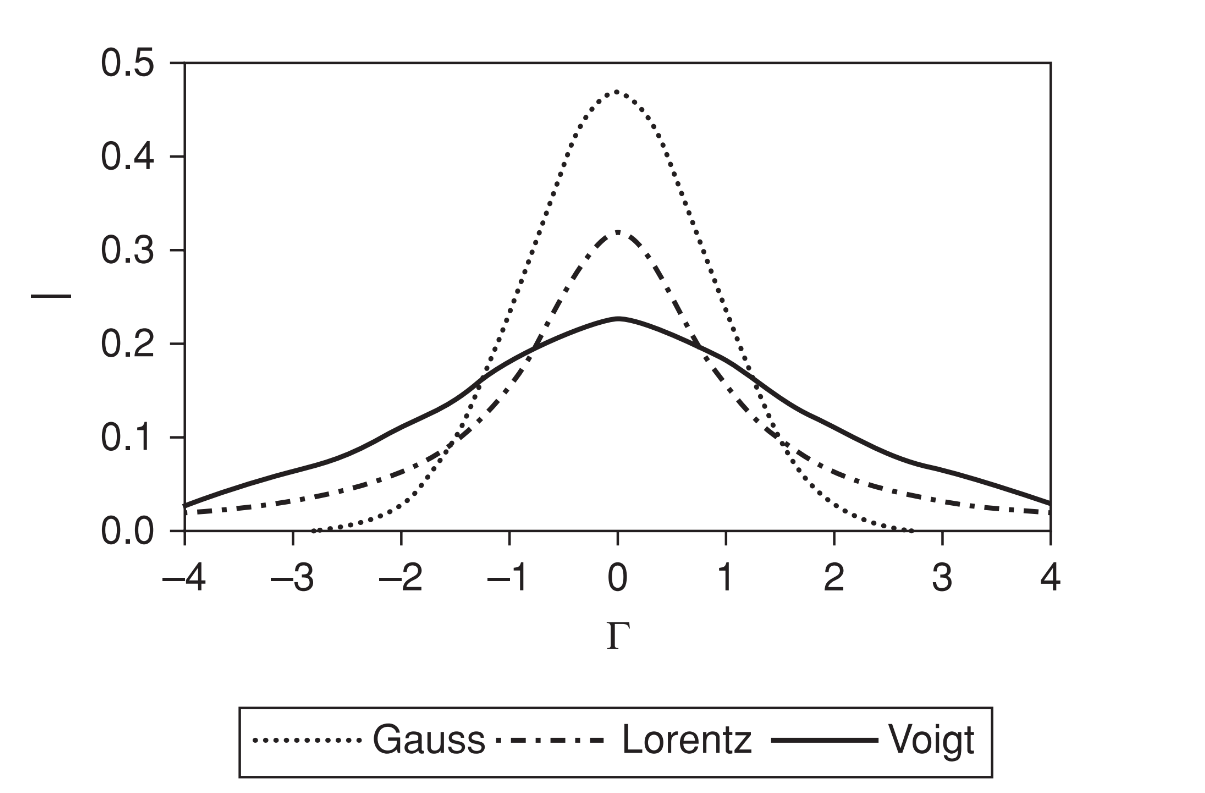
\includegraphics[width = 0.6\textwidth]{chapter_1/voigt.png}
    \caption{Plot of a Voigt profile.}
    \label{fig:voigt}
\end{figure}
[taken from https://scipython.com/book/chapter-8-scipy/examples/the-voigt-profile/]
\\
In normal conditions the main contributions of broadening in a LIBS plasma are due to Doppler and Stark effect. Natural line width is always present but usually the effect is so small that, even without the presence of other broadening mechanisms, it would not be resolved by commonly used LIBS spectrometer ($\Delta\lambda = 0.002\:nm$ for a $10\:ns$ transition at $500\:nm$).
\\
The Doppler width depends only on the temperature of the plasma and on the mass of the particles that are emitting the electromagnetic waves:
\begin{align}
    \Delta\lambda_{D}=7.2\times{10}^{-7}\left(T/M\right)^{1/2}\lambda_{o} \label{eq:doppler_eq}
\end{align}

The Stark effect will produce both a broadening and a shift, and both are dependent on the electron density ($N_e$) and can be used experimentally to obtain the parameter:

\begin{align}
    w_{\mathrm{total}}&\sim\left[1+1.75A\left(1-0.75r\right)\right]\left(n_{e}/{10}^{16}\right)w \label{eq:stark_width} \\ 
    d_{\mathrm{total}}&\sim\left[d/w+2.00A\left(1-0.75r\right)\right]\left(n_{e}/{10}^{16}\right)w \label{eq:stark_shift} 
\end{align}

\subsubsection{Plasma Opacity}
\label{subsubsec:plasma_opacity}
A plasma is defined as “optically thin” when the emitted radiation can freely escape from the plasma without being absorbed or scattered. This is a crucial characteristic to have in a plasma used for LIBS measurement, in this way the emitted radiation can be directly and more easily correlated with the atomic concentrations in the material.
\\
In general, the intensity of the radiation is given by:

\begin{align}
  I\left(\lambda\right)=\left[\varepsilon\left(\lambda\right)/\alpha\left(\lambda\right)\right]\left[1-\exp{\left(-\alpha\left(\lambda\right)L\right)}\right] \label{eq:intensity_radiation}  
\end{align}

Where $\varepsilon$ is the emissivity, $\alpha$ is the absorption coefficient and L is the plasma length in the direction of the observer. For an optically thin plasma we have that $\alpha$ is small and therefore:

\begin{align}
   I(\lambda)=[\varepsilon(\lambda)/\alpha(\lambda)][\alpha(\lambda)L]\varepsilon(\lambda)L \label{eq:intensity_radiation_approx}  
\end{align}

For strong lines, self-absorption will manifest as a flat-topped profile while for other cases certain lines will appear to have a dip in the middle of the curve, in that case the line is called “self-reversed”. 

\begin{figure}[H]
    \centering
    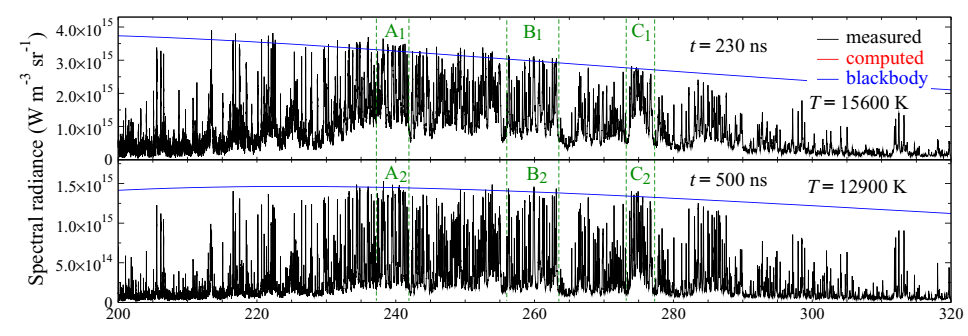
\includegraphics[width = \textwidth]{chapter_1/self_absorption_flat.png}
    \caption{Flat-topped profile of a spectrum caused by self-absorption.}
    \label{fig:self_absorbed_flat}
\end{figure}

\begin{figure}[H]
    \centering
    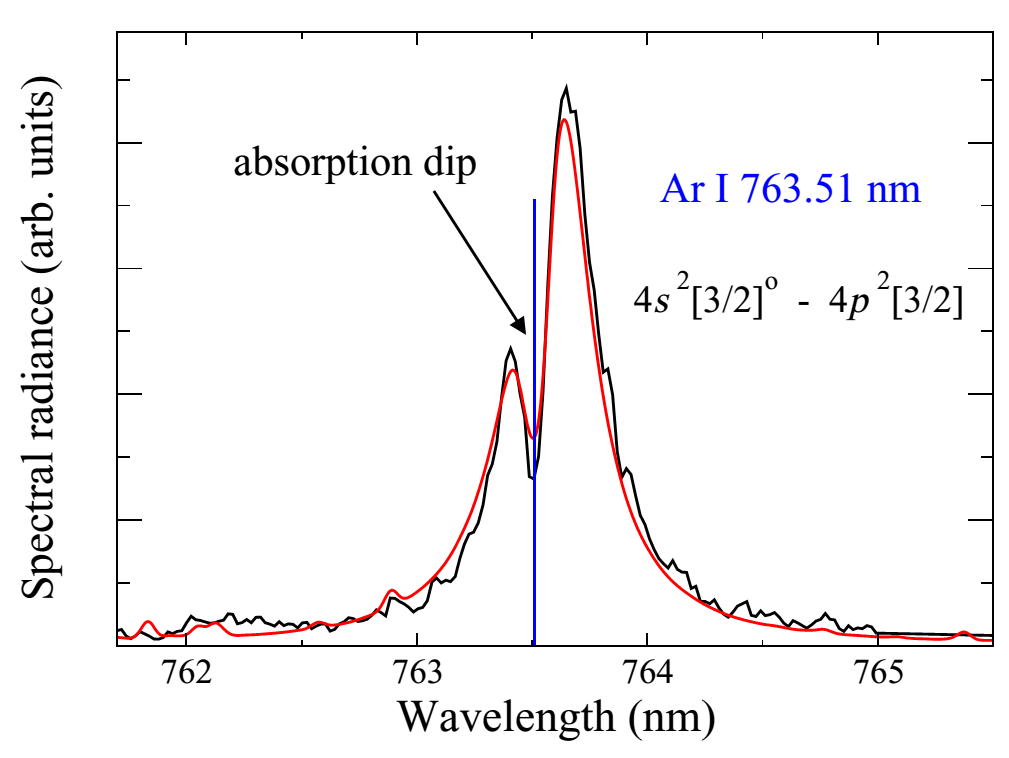
\includegraphics[width = 0.8\textwidth]{chapter_1/self_absorption_peak.png}
    \caption{Self-reversed line caused by high optical thickness.}
    \label{fig:self_absorbed_peak}
\end{figure}
[Taken from jorg's powerpoint]

\subsubsection{Thermodynamic Equilibrium and Plasma Temperature}
\label{subsubsec:thermodynamic_eq}

If a plasma is in thermodynamic equilibrium, it means that all the individual species (electrons, ions, atoms, and molecules) can be described by the same temperature. This condition is generally not true; collisions between particles of the same mass have a much higher probability of equally distributing the kinetic energy after the interaction, this leads to the different species achieving equilibrium individually but not globally, and in general the plasma will be characterized by a different temperature for each one of them.

\begin{figure}[H]
    \centering
    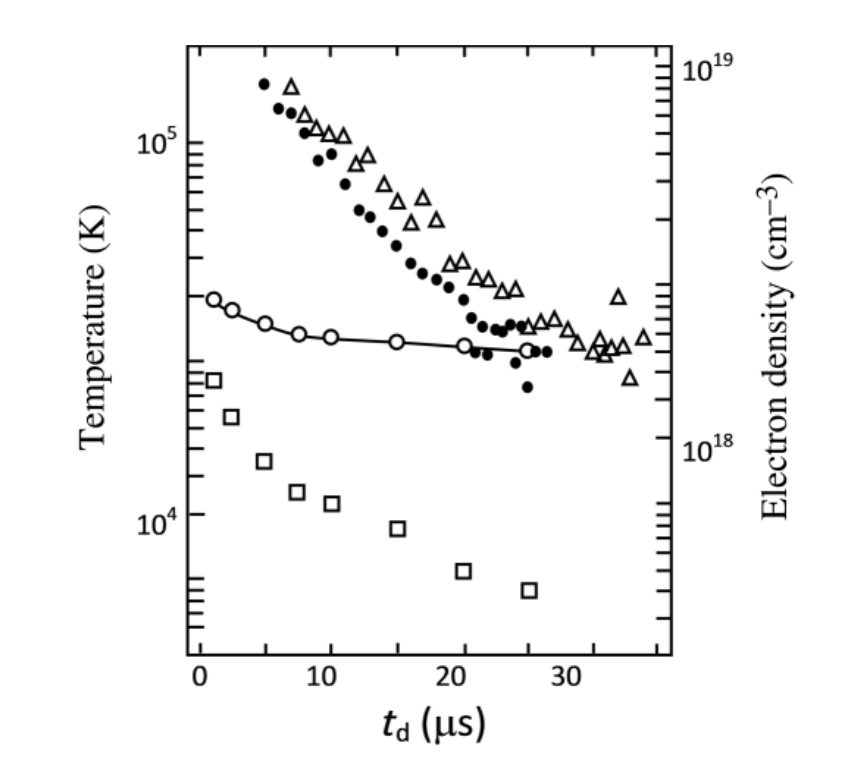
\includegraphics[width = 0.8\textwidth]{chapter_1/electron_equilibrium.png}
    \caption{Convergence of electron temperature for an air plasma.}
    \label{fig:electron_equilibrium}
\end{figure}
[taken from the HANDBOOK of libs]\\
In Figure~\ref{fig:electron_equilibrium} we can see electrons reaching global equilibrium $25\:\mu s$ after the incidence of the pulse. By looking at the Figure~\ref{fig:time_plasma_emission} is evident that the intensity of the emission decays exponentially, and at $25\: \mu s$ the magnitude is already negligible. For this reason, the condition of global thermodynamic equilibrium is not usually required, and it is enough to demand the “Local Thermodynamic Equilibrium” (LTE), where we assume that the equilibrium is reached only locally in small portions of the plasma.
\\
An important criterion to test if a plasma is in thermodynamic equilibrium is the so-called “McWhirter criterion”; is used to see if the electron density is high enough for collision to dominate the population of levels. 
\\
The McWhirter criterion can be expressed by this relation: 

\begin{align}
   n_{e}>1.6\times{10}^{12}T^{1/2}\left(\Delta E\right)^3 \label{eq:mcwhirter_criterion}  
\end{align}
Where $\delta E$ is the energy of the first level above the ground state.
\\
A more precise way to check if the LTE condition is valid is to see if the plasma respects the theoretical temperatures calculated by the Boltzmann and Saha equations. 
For $N_o$ electrons distributed between two levels $i,j$ with respective populations $N_i$ and $N_j$, the relative population will be given by the Boltzmann distribution:
\begin{align}
   N_j/N_{o}=\left(g_j/Z\right)\exp{\left[-E_j/kT\right]}N_j/N_i=\left(g_j/g_i\right)\exp{\left[-\left(E_j-E_i\right)/kT\right]} \label{eq:boltzmann_distribution}  
\end{align}
Where $g_{i,j}$ are the statistical weights and $Z$ is the partition function.
\\
The spectral radial intensity for a given transition with an energy $\lambda$ is then given by: 

\begin{align}
   I=hvAN/4\pi=\left(hcN_0gA/4\pi\lambda Z\right)\exp{\left[-E/kT\right]} \label{eq:spectral_radial_int}  
\end{align}
Where A is the transition probability (Einstein coefficient).
\\
A better and more reliable way to measure the temperature is to use more than one line simultaneously and perform an analysis graphically. By rearranging the previous expression, we obtain:
\begin{align}
   \ln{\left(I\lambda/gA\right)}=-E/kT-\ln{\left(4\pi Z/hcN_0\right)} \label{eq:bolzmann_plot_eq}  
\end{align}

In this way there is a linear dependence between the logarithm of a parameter related to the line intensity and the transition energy, with an angular coefficient $1/kT$. By plotting various transitions of the same element, if the data follows a linear trend, the assumption of LTE is valid, and it is possible to obtain the temperature from the slope.

\begin{figure}[H]
    \centering
    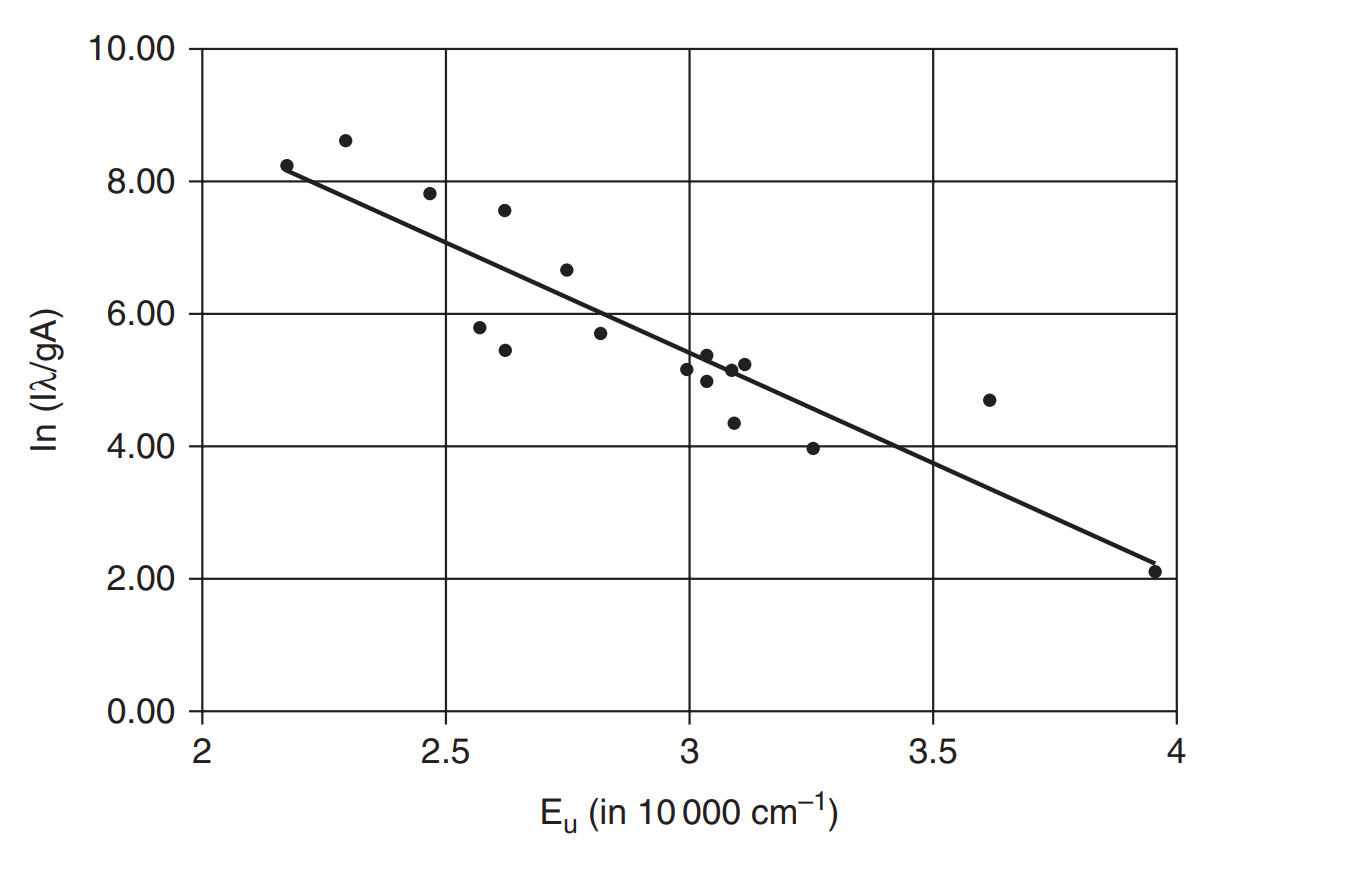
\includegraphics[width = 0.7\textwidth]{chapter_1/boltzmann_plot.png}
    \caption{Multi-line Boltzmann plot based on uranium data.}
    \label{fig:boltzmann_plot_example}
\end{figure}
[taken from the HANDBOOK of libs]\\
While the Boltzmann equation regulates the different populations of energy levels in neutral atoms and molecules, the Saha equation describes the relative populations of different ion stages of a certain atomic species in LTE. The expression of the equation is:

\begin{align}
   \frac{N\left(Z,0\right)}{N\left(Z-1,0\right)}n_{e}=\left(2\left(2\pi m k T\right)^{3/2}/h^3\right)\left(gA\left(Z,0\right)/gA\left(Z-1,0\right)\right)\exp{\left[-\Delta E/kT\right]} \label{eq:saha_equation}  
\end{align}

Where $N(Z,0)$ and $N(Z-1,0)$ represent the population of the ground state of the ion stages $Z$ and $Z-1$ respectively and $\Delta E$ is the ionization energy. It is important to underline that in this case the electron density must be known to apply the expression.
\\
Both equations can be used in conjunction to test for LTE and to estimate the temperature.

\subsection{LIBS Setup Components}
\label{subsec:libs_setup_component}
[taken from Fundamentals and applications]
In a LIBS analysis, four main devices are involved:
\begin{enumerate}
    \item High-energy pulsed laser: Typically operating with nanosecond-duration pulses, the laser is directed at the sample that needs to be studied, causing surface evaporation, and inducing plasma formation.
    \item Spectrometer: Responsible for both diffracting the light collected through an appropriate optical system to obtain its spectral signature and then detecting the intensity of the light at each wavelength. This can be achieved using various devices such as photomultiplier tubes (PMT), photodiode arrays (PDA), or charge-coupled devices (CCD). 
    \item Computer: Processes the acquired spectrum, allowing for further analysis.
\end{enumerate}

Precise time control is crucial in LIBS applications, plasma undergoes various stages in its lifetime that need to be managed to improve the spectral signature.
\\
The selection of the laser, combined with the spectrometer, detector, and time control unit, must be adapted according to the surrounding environmental conditions and the type of materials to analyze.

\subsubsection{Laser}
\label{subsubsec:laser_setup_component}
The laser is the central component of the LIBS system, providing the energy necessary to induce plasma formation. Consequently, the characteristics of the plasma are closely tied to the properties of the laser. The laser influence on the evolution of the plasma occurs both during the interaction between the laser pulse and the sample surface and during the interaction of the laser pulse with the generated plasma plume.
\\
The main parameters related to the laser source include:
\begin{itemize}
    \item Wavelength.
    \item Pulse energy.
    \item Pulse duration (typically in the nanosecond range).
    \item Repetition rate (number of pulses per second) or pulses per measurement.    
\end{itemize}

\paragraph{Wavelength}
\label{par:wavelength_setup_component}
After the initiation of the ablation process, the laser pulse interacts with the gas plume composed of ablated material from the sample's surface. As previously discussed, when the energy of the incoming photon exceeds the bond energy of the electron, photoionization occurs.
\\
Plasma formation primarily occurs through two processes: inverse bremsstrahlung and photoionization. In inverse bremsstrahlung, free electrons gain kinetic energy by absorbing photons from the incident laser light during collisions with atoms and ions.
\\
Inverse bremsstrahlung is more favorable for infrared (IR) and longer wavelengths. [Fundamentals and applications, 26] Consequently, laser sources with shorter wavelengths transfer energy to the material more efficiently, leading to higher ablation rates since the effect of plasma shielding is lower. However, for the same reason plasma ignition is less efficient with shorter wavelengths, resulting in a higher threshold for plasma formation. On the other hand, longer wavelengths will transfer energy to the plasma more efficiently but resulting in lower surface ablation.
\\
A variety of lasers are utilized in LIBS systems, with solid-state Nd: YAG lasers being commonly employed. This choice is attributed to their relatively low cost, ease of maintenance, and compact size, enabling their integration into systems of various sizes. The Nd: YAG laser typically operates at a fundamental wavelength of $1064\:nm$ with a pulse temporal width between $6$ and $15\:ns$. However, it is common for these lasers to operate at higher harmonics, such as the second harmonic at $532\:nm$, the third harmonic at $355\:nm$, or the fourth harmonic at $266\:nm$. These higher harmonics are less powerful and feature shorter pulse durations, typically between 4 and $8\:ns$ [Fundamentals and Applications].

\paragraph{Pulse Energy}
\label{par:pulse_energy_setup_component}
Both ablation and plasma ignition are significantly influenced by the energy and temporal duration of the laser pulse. In LIBS applications, the energy delivered to the sample per unit area is a more critical parameter than the absolute energy value of the laser pulse. Therefore, the primary physical quantities used in the analysis are Fluence, which represents energy per unit area (measured in $J/cm^2$), and Irradiance, which represents power per unit area (measured in $W/cm^2$).
\\
For this reason, fluence and irradiance can be adjusted both by varying the energy of the pulse and by tuning the focal length of the system, in order to change the spot size of the laser on the sample surface.
\\
Variations in pulse energies and focusing distances will also impact the shape and temporal evolution of the plasma plume [Analytical Chemistry LIBS]. At high irradiances, the plasma will contain more ablated material and possess greater internal energy, allowing it to expand with a hemispherical shape by pushing the surrounding air farther away. Conversely, at lower fluence levels, the plume will expand with less energy, resulting in a shape similar to a disk that evolves radially and remains closer to the surface of the sample.
\paragraph{Laser Pulse Duration}
\label{par:laser_pulse_duration_setup_component}

Regardless of their duration, laser pulses typically meet the necessary conditions for ablating targets. The rate of energy deposition will, indeed, surpass the rate of energy redistribution and dissipation through the sample lattice, leading to extremely high temperatures in those regions where energy absorption occurs.
\\
The nature of ablation is strongly influenced by the duration of the laser pulse.
When using lasers that generate pulses in the femtosecond regime, non-thermal processes dominate the ionization. This means that since the pulse duration is too short to induce thermal effects in the sample's matrix structure, other mechanisms are therefore responsible for ionizing the atoms. In this case, the pulse carries a significant amount of energy, and phenomena such as photochemical absorption, multi-photon absorption, tunneling, and avalanche ionization occur to excite the sample. 
\\
The absence of thermal effects results in the formation of a crater with sharply defined edges, without any melted or deposited materials surrounding it. After the laser pulse, only a very hot electron gas and an essentially undisturbed lattice remain.
\\
Conversely, when using laser pulses in the nanosecond regime, different effects come into play. The time required for electron-lattice heating is approximately $1\:ps$ [Fundamentals and Applications], much shorter than the duration of the pulse. As a result, thermal effects dominate the ionization process.
\\
After the interaction with the laser pulse, the material undergoes transient changes in thermodynamic states, transitioning from solid to liquid and ultimately into a plasma state [Analytical Chemistry].
\\
In simple terms, the pulse initially melts and vaporizes the surface, with the increasing temperature eventually leading to the ionization of atoms. If the irradiance is sufficiently high, both thermal and non-thermal effects will contribute to the ionization of the sample. Between 1 and $10 \: ns$, the plasma becomes opaque to laser radiation [Fundamentals and Applications]. As a result, the latter part of the pulse does not significantly contribute to surface vaporization. Instead, it interacts with the already generated plasma plume, potentially being absorbed, or reflected. This interaction leads to a decrease in the ablation rate, a phenomenon known as "Plasma Shielding." 
\\
Plasma Shielding is highly dependent on environmental conditions such as pressure and the composition of gases in the atmosphere, as well as experimental factors including laser wavelength and irradiance.
\\
When using nanosecond pulses, the generated craters typically exhibit melted and deposited material around them, as seen in the SEM images shown in Figure~\ref{fig:craters_laser_duration}:
\begin{figure}[H]
    \centering
    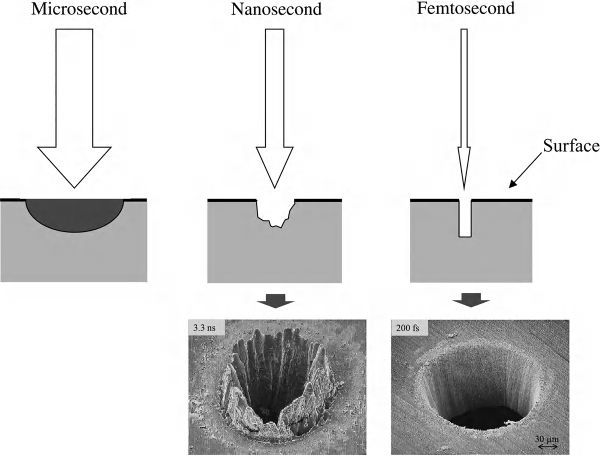
\includegraphics[width = 0.7\textwidth]{chapter_1/craters_laser_duration.jpg}
    \caption{SEM images of craters produced by different types of laser.}
    \label{fig:craters_laser_duration}
\end{figure}
[taken from the HANDBOOK of LIBS]
\\
At the same time, the plasma is reheated, resulting in longer plasma lifetimes and larger plasma plume sizes [Fundamentals and Applications].
\subsection{Spectra Evaluation}
\label{subsec:spectra_evaluation}
Once the plasma has been ignited, the emitted light is collected by a detector, which creates a spectrum with the intensities of the measured light on the $y$ axis, and the wavelengths on the $x$ axis. 
\begin{figure}[H]
    \centering
    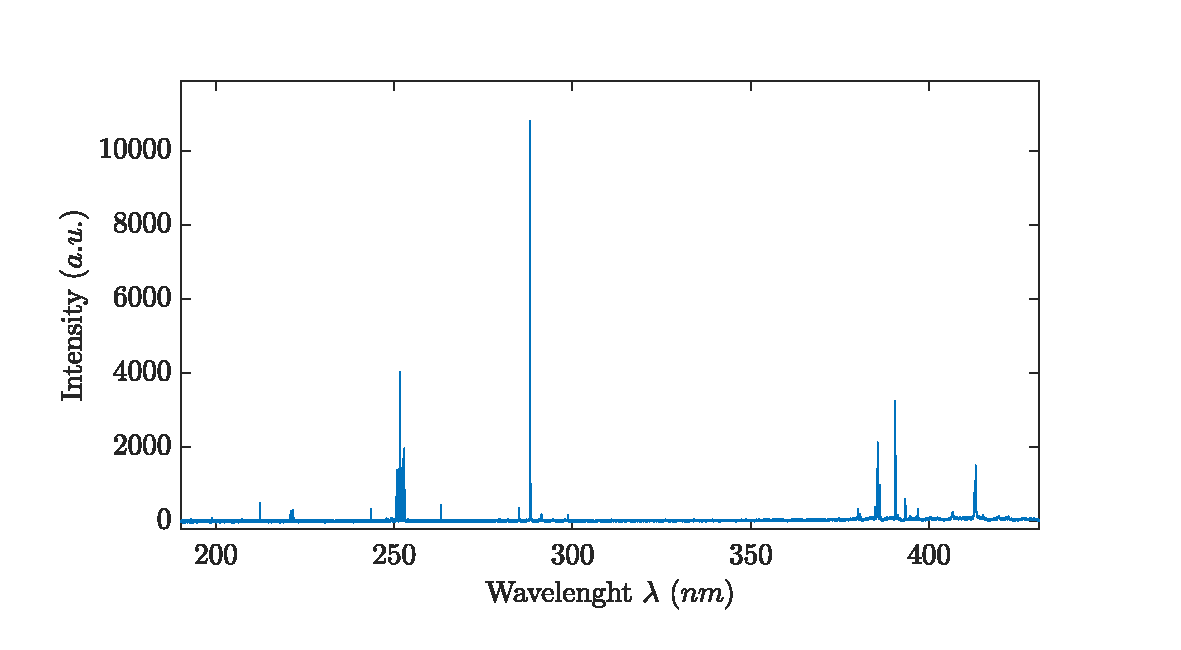
\includegraphics[width = \textwidth]{chapter_1/generic_spectrum.pdf}
    \vspace*{-30pt}
    \caption{LIBS spectrum of a pure silica sample we measured.}
    \label{fig:generic_spectrum}
\end{figure}
This spectrum may contain emission lines from atomic species, as well as continuous radiation resulting from bremsstrahlung [Fundamentals and Applications].
\\
Continuous radiation can hide emission lines, so efforts should be made to minimize its detection. 
\\
Since the energy of a transition is characteristic of the particle species, analyzing photon energies can reveal the composition of the plasma.
Accurate identification of LIBS emission lines is essential for determining the elemental constituents of a sample. The analysis of the LIBS spectrum will reveal elements present at concentrations above the method's minimum detectable limit (LOD).
\\
The most important spectral region for LIBS typically spans from 200 to $800\: nm$, where most elements exhibit strong emission lines. In addition to emission from atoms and ions, emission from simple molecules may also be observed in the samples. Generally, high concentrations of the elements composing the molecules must be present for molecular emission to be observed.
\\
Currently, LIBS is limited by problems of low reproducibility, with a resulting poor accuracy. Problems associated whit shot to shot variations in plasma conditions, which are caused by the stochastic nature of the laser source and light-matter interaction, seem to be the major cause of this effect [Applications of single-shot laser]. For this reason, a single measurement is usually obtained by averaging hundreds of different shots.
\\
More details on spectra evaluation will be presented in %Chapter~\ref{}

\chapter{Glass Manufacturing}
\label{ch:experimental_techniques}

\section{Grinding of Glass}
\label{sec:grinding_glass}

The manufacturing process of polished glass pieces typically begins with grinding, which, thanks to its ability to achieve surface flatness while maintaining high MRRs on hard and brittle materials, is considered one of the most important and feasible machining technologies. However, grinding can induce surface and subsurface damage on the glass sample. Consequently, chemical mechanical polishing (CMP) is employed to eliminate these residual defects [CMP of glass disk].
\\
Grinding too is a complex process, especially when applied to glass due to the nature of the material. The most used abrasive materials are silicon carbide or diamond grinding wheels [Grinding of Glass: the mechanics of the process *(GoG)*]. 
\\
Previous research shows that both permanent viscous flow and brittle fracture can occur during the grinding of glass surfaces. 
Viscous flow is the main grinding mechanism when using silicon carbide. On the contrary, when using diamond grinding wheels, glass is ground mostly through brittle fracture of particles from the surface.

\subsection{Non-Newtonian Flow of Glass Particles}
It is widely recognized that glass can be made to flow without fracturing under significant hydrostatic compressive stresses, even at ambient temperature [GoG]; this can happen because the local surface temperature in the grinding zone can easily exceeds the glass's softening point. The pressure conditions, favorable for the flow of glass, are also expected to exist at the cutting edge of an abrasive grain during grinding.
\\
It has also been observed that most of the grinding energy is dissipated in the material by viscous deformation [GoG]. For this reason, glasses with high softening temperatures also have a high specific grinding energy, that is defined as the proportionality constant between the work expended in the process and the rate of material removal.
\\
Additionally, it has been observed that there is a correlation between the increase in specific grinding energy and the decrease in particle grain sizes [GoG].
\\
Numerous experimental investigations have clearly demonstrated that when soda-lime glass is subjected to sufficiently high axial stress or pressure, it exhibits a nonlinear mechanical response, and an irreversible deformation takes place, a phenomenon known as inelasticity or material nonlinearity [Material Nonlinearity and Inelasticity] [non-Newtonian viscous flow]. Studies of the viscosity of stable soda-lime glass under high shear stress have revealed a non-Newtonian viscosity of the pseudoplastic type. In this behavior, if the applied stress rate exceeds a certain threshold value, catastrophic failure of the material occurs, leading to the formation of numerous cracks and an eventual brittle fracture of the glass sample [Non-Newtonian Viscous Flow].
\\
The interpretation of this non-Newtonian behavior is attributed to atomic structural rearrangements within the glass material. These rearrangements play a significant role in determining the material's mechanical response under high stress conditions, ultimately influencing its flow and fracture characteristics during the grinding process.
\section{Chemical Mechanical Polishing}
\label{sec:CMP}
Chemical mechanical polishing (CMP) has been a widely used planarization method in various industries, including integrated circuits manufacturing and glass surface polishing, for many decades. The effectiveness of CMP in achieving planar, smooth, and damage-free surfaces is influenced by numerous factors related to the sample carrier structure, polishing pad, slurry composition, and other process parameters. Since both chemical and mechanical actions play a role in CMP, and since they are influenced by multiple variables, understanding the complexity of the CMP mechanism is still a great challenge and is an actively researched topic.
\\
CMP aims to produce planar surfaces on target materials by removing micro and nano-sized particles, sometimes acting even on the atomic-scale; with the goal of achieving sub-nanometer level roughness while minimizing surface and subsurface damage [CMPTE]. The surface smoothing effect observed in CMP is attributed to various mechanisms, including the non-Newtonian flow of glass material, fretting and mechanical abrasion caused by friction between the glass and the polishing tool, and chemical reactions leading to surface decomposition.
\\
In general, mechanical abrasion and chemical removal are typically the predominant mechanisms, leading to the use of the term: "chemo-mechanical polishing" [Gerhard et al. Appl Surf Sci].
\\
Mechanical removal is mostly based on the interaction of the glass surface with abrasive grains, such as cerium oxide or aluminum oxide, present in an aqueous polishing slurry. On the other hand, chemical removal involves complex processes such as diffusion of water molecules into the glass sample, redeposition of silica on the surface during polishing, and diffusion of polishing agents into the surface of the glass [Cook, 1990].
\\
Polishing is not only needed to obtain a transparent surface of an optical glass component with the required accuracy, but also to remove digs, pits, and microcracks induced by the previous processes to obtain smooth surfaces that minimize scattering [Optics Manufacturing (Gerhard)].

\subsection{CMP Technique}
\label{subsec:cmp_technique}

Chemical mechanical polishing (CMP) is a process that, by definition, combines chemical and mechanical actions to enhance the material removal rate (MRR), which quantifies the amount of material removed per unit time. The MRR is influenced by various factors including the system configuration, the properties of the abrasive pad, and the composition of the polishing suspension employed.
\\
Depending on the layout of the polishing machine, different approaches and principles can be applied for polishing.
\\
There are four main types of commercially available CMP equipment commonly used in industry, as shown in Figure~\ref{fig:cmp_equipment}: 
\begin{figure}[H]
    \centering
    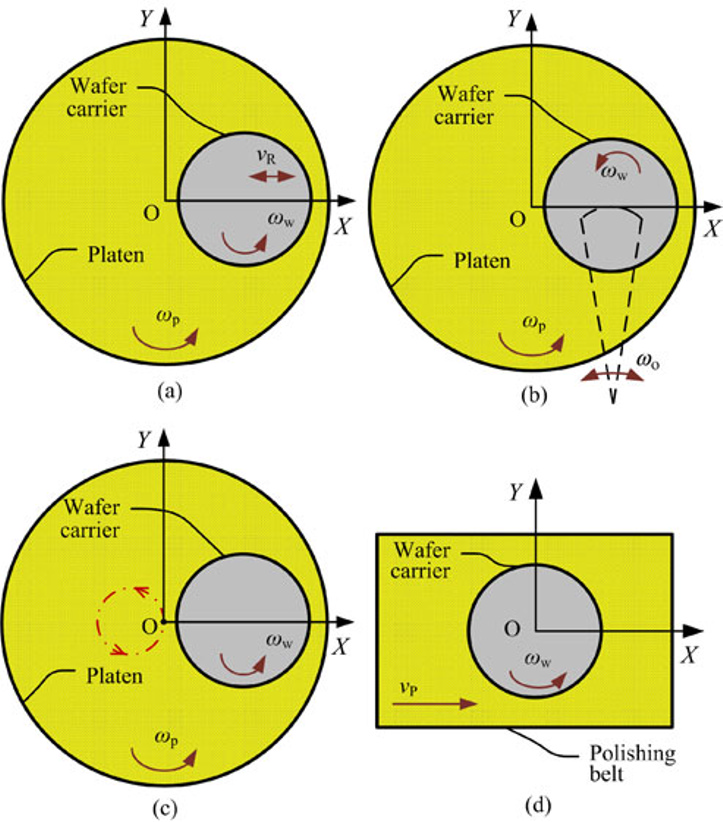
\includegraphics[width = 0.4\textwidth]{chapter_2/cmp_equipment.png}
    \caption[Schematic of different types of CMP equipment.]{ Schematic of different types of CMP equipment: (a) rotary type, reciprocation mode, (b) rotary type, oscillation mode, (c) orbital type, and (d) linear type.}
    \label{fig:cmp_equipment}
\end{figure}
[taken from CMP theory and experiments]

\begin{enumerate}
    \item Rotary type polisher with a sample carrier featuring a reciprocating motion along the platen diameter.
    \item Rotary type polisher with a sample carrier exhibiting an oscillatory motion.
    \item Orbital type polisher with the platen having an orbital rotation.
    \item Linear type polisher equipped with a linear motion belt as the polishing pad.
\end{enumerate}
The movement of the carrier and the platen generates the necessary relative motion for the polishing process, while a slurry, containing particles and chemical solutions, is delivered onto the pad to act as the abrasive [CMPTE]. Through the combined chemical actions of the solutions and the mechanical actions of the particles, micro material removal occurs, enabling surface polishing and finishing to be realized.
\\
The MRR, non-uniformity, and surface quality are key indicators of machining and CMP process efficiency. These parameters are influenced by some major factors such as the system configuration, process variables (e.g., down pressing force of the sample on the pad, relative velocity of the pad), and consumables (e.g., slurry concentration). The synergetic interaction of these input variables determines the final polishing results by affecting the sample-pad interaction and material removal process. 

\subsection{Modeling of CMP}
The removal rate in CMP is determined by several parameters at the sample-pad interface, including pressure, temperature, and slurry distribution over the active surface. Many process variables, such as sample pressing downforce, pad rotation speed, slurry characteristics and the employed pad material, can influence the final polishing outcomes [CMPTE].
\\
A theoretical description of the polishing of optical glasses is thus a complex task since such polishing processes are based on different interacting mechanisms. These different mechanisms have been described by some models: the removal, the flow, the chemical, and the fretting hypothesis [Optics Manufacturing (Gerhard)].
\\
Under the removal hypothesis, the sharp edges of the abrasive particle grains of the polishing agent enter in contact with the surface of the glass digging out small particles. Since these interactions preferentially target the roughness peaks of the working surface, a smoothing effect is obtained over time [Optics Manufacturing (Gerhard)].
\\
The flow hypothesis says that in addition to the mechanical removal by abrasion, the polishing agent grains also perform an irreversible displacement of the glass material. Here, due to the friction between the work piece surface and the polishing pad and grain, the local temperature can rise above the softening point of the glass and as a result, roughness peaks are dislocated into roughness valleys or digs by material flow. 
\begin{figure}[H]
    \centering
    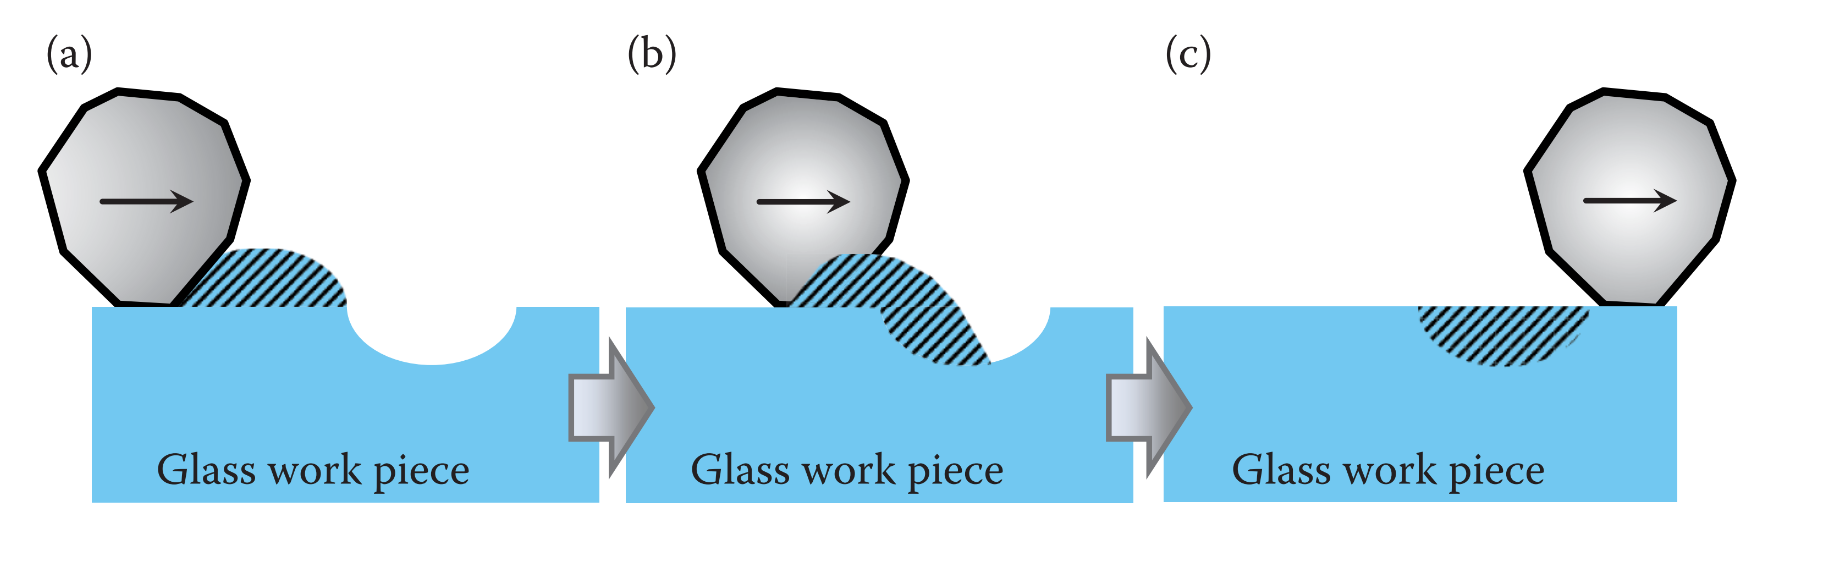
\includegraphics[width = \textwidth]{chapter_2/flow_hypothesis.png}
    \caption[Visualization of the flow hypothesis.]{ Visualization of the flow hypothesis; roughness peaks (dashed structure) are softened by wear in the course of the polishing process (a) and dislocated into roughness valleys or digs (b), consequently resulting in a leveling of the surface (c).}
    \label{fig:flow_hypothesis}
\end{figure}
[image taken from optics manufacturing Gerhard]
Under the chemical hypothesis are described the chemical reactions that take place on the surface of the target glass sample. Such reactions are supported by hydrolytic scission of bonds of the glass network [Optics Manufacturing (Gerhard)] according to Equation~\ref{eq:hydrolytic_scission}:
\begin{align}
\ce{(SiO2)_x + 2H2O <-> (SiO2)_{x-1} + Si(OH)4} \label{eq:hydrolytic_scission}
\end{align}
The rate of the reaction is controlled by the diffusion of water molecules at the surface of the glass [Cook, 1990]. The depth of this diffusion layer can be estimated, after a given time “$t$”, by the relation: 
\begin{align}
    d_{dif}\ \approx\ 2\sqrt{Dt} \label{eq:diff_length}
\end{align}
Where D is the diffusion coefficient of water into glass and its value can range from $10^{-15} \:cm^2/s$ to $10^{-18}\: cm^2/s$ : (Nogami and Tomozawa, 1984; Lanford et al., 1985).
\\
As a result of this phenomenon, hydrated silica is deposited on the sample surface during polishing, consequently leading to the formation of a silica gel layer [Optics Manufacturing (Gerhard) (Iler, 1979; Cumbo and Jacobs, 1994)] that contributes to surface smoothing, since it can accumulate in digs and scratches filling those geometric surface defects. 
\\
The last studied mechanism is based on the material removal due to fretting, arising from the synergy between two physical factors: the contact pressure of the polishing tool on the glass surface and their relative movement [Optics Manufacturing (Gerhard) (Dimatteo, 1997)]. This early model, developed by Frank W. Preston in the late 1920 (Preston, 1927) describes the MRR through an empirical equation as follows:
Formula (8.4) in [Optics Manufacturing (Gerhard)] and [CMPTE]
\begin{align}
    MRR=kPV \label{eq:material_removal}
\end{align}
Here, “$k$” is an empirical constant determined from experimental data, P is the pressure applied to the sample and $V$ is the relative velocity between the glass and the polishing tool.
\\
This equation only considers the mechanical contributions to the MRR, neglecting the chemical actions. In this way, the polishing process can be described as a simple two body wear problem, where the target sample is pressed down on a polishing pad and moving at a fixed speed.
\\
To increase the accordance with experimental data, an alternative expression for the Preston equation have been proposed: $MRR=kP^\alpha V^\beta$[CMPTE]; where the dependence of the $MRR$ relative to the pressure and velocity is no longer linear. However, this model still fails to correctly describe processes where chemical interactions are crucial.

\section{Polishing Elements}
\label{sec:polishing_elements}
In the polishing process a resilient pad, a target sample to be polished, and an abrasive slurry are the key components. The process involves pressing a glass sample face down onto a rotating polishing pad while a slurry containing abrasive particles and chemical additives flows between them. This mechanical and chemical action removes material from the sample, resulting in a smoother surface.
\subsection{Polishing Pad}
Different types of pads can be utilized for polishing, even though traditionally the typical polishing pad was made of pitch [Optics Manufacturing (Gerhard)], a natural viscoelastic polymer, also known as bitumen or asphalt, derived from petroleum or tar. Today polishing pads are typically made of porous polyurethane [CMPTE] with additional components added to tune the pad hardness [CMPTE 4]. This material is capable of higher process velocities, and it is less sensitive to temperature changes [Optics Manufacturing (Gerhard)]. 
\\
The hardness of the pad is a critical property that can influence both the material removal rate (MRR) and the uniformity of polishing [CMPTE]. Different applications and types of target materials may require either hard or soft pads.
\\
Both the bulk of the pad and the surface are full of micropores, which are useful for retaining the abrasive particles of the slurry; these micropores play a crucial role in the polishing process by facilitating the interaction between the pad, the slurry, and the sample. As shown in Figure~\ref{fig:hard_soft_pad}
\begin{figure}[H]
    \centering
    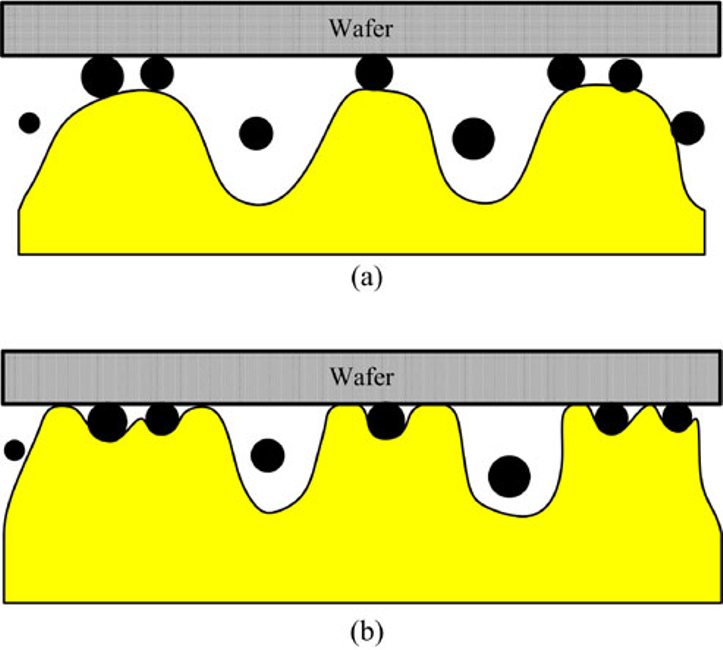
\includegraphics[width = 0.6\textwidth]{chapter_2/hard_soft_pad.png}
    \caption[Comparison between a hard pad and a soft pad.]{ Contact status of (a) hard pad, and (b) soft pad. }
    \label{fig:hard_soft_pad}
\end{figure}
During CMP, the physical properties of the pad, such as hardness and surface roughness, are expected to change due to mechanical loads and chemical reactions occurring during the polishing. These changes could significantly impact the process, so they should be limited to ensure consistent results.

\subsection{Polishing Suspension (Slurry)}
\label{subsec:polishing_slurry}

The slurry used in CMP is a complex mixture consisting of abrasive materials dispersed in water along with various chemicals, including oxidants, inhibitors, and bases to adjust the pH. Abrasive particles such as \ce{SiO2}, \ce{CeO2}, and \ce{Al2O3}, with sizes ranging from 10 nanometers to some micrometers [Optics Manufacturing (Gerhard)], are commonly used in industrial CMP processes. The mass concentration of the polishing agent relative to the total slurry usually spans from 5\% to 30\% [Bliedtner and Gräfe, 2008].
\\
The choice of a particular polishing agent depends on the material of the work piece [Optics Manufacturing (Gerhard)], while the properties of the abrasive particles, such as the size distribution, chemical composition, and concentration, as well as the pH of the slurry, will have a significant impact on the material removal rate ($MRR$), uniformity, and surface quality of the polished material [CMPTE]. For example, at pH values of 3.0 and 10.0, the material removal is primarily driven by chemical corrosion, while at a pH around 7.0, the mechanical action of abrasive particles becomes the dominant factor contributing to the $MRR$. [Effects of chemical additives of CMP]
\\
During CMP, the slurry plays a crucial role at the interface between the wafer and the polishing pad. The flow of slurry brings abrasive particles and chemicals to the interface, where they initiate the polishing process by removal or material flow [Optics Manufacturing (Gerhard)]. The slurry will form a lubricating film, reducing friction forces between the wafer and pad, and the fluid presence can also help support some of the downforce, thereby relieving pressure from the pad [CMPTE].
\\
Physical models have shown that in slurry with a size distribution of abrasive particles, only the larger particles make direct contact with the pad and the sample, leading to effective material removal [Effect of chemicals on CMP of glass substrates]. 

\section{Side Effects of Polishing}
\label{sec:polishing_side_eff}

The uniformity of glass substrate surfaces in terms of index of refraction, chemical composition, and roughness is crucial in many different applications. However, during the manufacturing process, from rough grinding to fine polishing, nonuniform surfaces can arise. This is due, for example, to the presence of contaminants inside the glass, caused by residues of operating materials used during manufacturing as, most commonly, polishing agents.
\\
One significant chemical mechanism, happening on the surface of the sample during CMP, is the formation of a silica gel layer, also known as the redeposition layer [Gerhard et al appl opt 2017].
\\
This layer forms as water penetrates the glass surface, leading to hydrolytic scission of the glass network, which results in the formation of a thin layer consisting of hydrated silica, or silanol. During the growth of this layer on the surface, also known as Beilby layer, residues from polishing agents and other elements from the polishing suspension can remain embedded within it [Gerhard et al appl surf sci].
\\
For example, some studies [Kozlowski] have shown that aluminum from corundum-based abrasives can exceed a mass fraction of 1000 ppm on the glass surface. This retention occurs as particles from the polishing slurry accumulate within surface defects such as digs, scratches, and microcracks formed during earlier manufacturing steps [Gerhard et al Appl Opt 2017].

\begin{figure}[H]
    \centering
    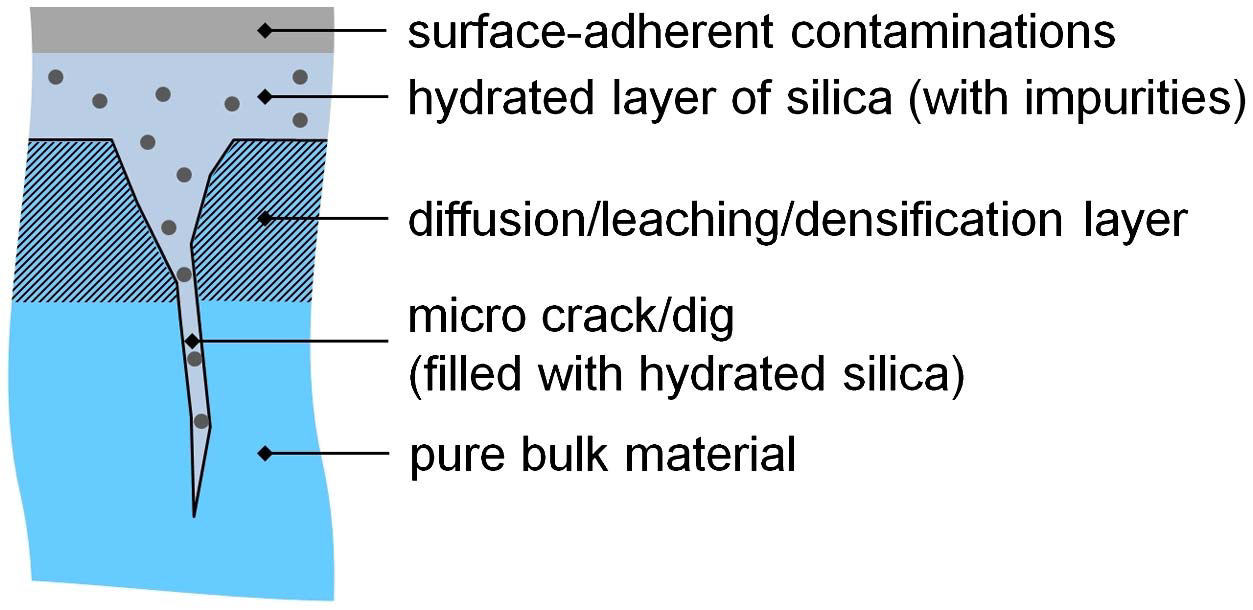
\includegraphics[width = 0.6\textwidth]{chapter_2/micro_cracks.png}
    \caption[Schematic of a surface defect generated during optics manufacturing.]{ Schematic presentation of a typical surface defect generated
during classical manufacturing of optical surfaces. }
    \label{fig:micro_cracks}
\end{figure}
[taken by Gerhard app optics]
\\
As a result of these processes, visually clean polished glass surfaces can exhibit significant optically active contaminations [Gerhard et al Appl Opt 2017]. These contaminations may include surface adherent contaminants such as hydrocarbonaceous compounds and residues from polishing agents. The remaining silica gel layer and contaminants on the surface can also lead to negative effects such an increase in near-surface absorption consequently lowering the laser-induced damage threshold [Optics Manufacturing (Gerhard)].

\section{Diffusion}
\label{subsec:diff}

As already mentioned in Chapter~\ref{sec:CMP}, diffusion is a core process in optics manufacturing; following is a brief exposition on the main characteristics of the mechanism.
\\
Diffusion is a physical and time dependent mechanism that drives the flow of particles from a low concentration portion of a medium to a high concentration one. The process is purely thermodynamical, the difference between the chemical potential, i.e. the potential associated with the concentration of particles, causes a difference between the Gibbs free energy of the two areas and leads to the flow of material in order to achieve equilibrium.
\begin{figure}[H]
    \centering
    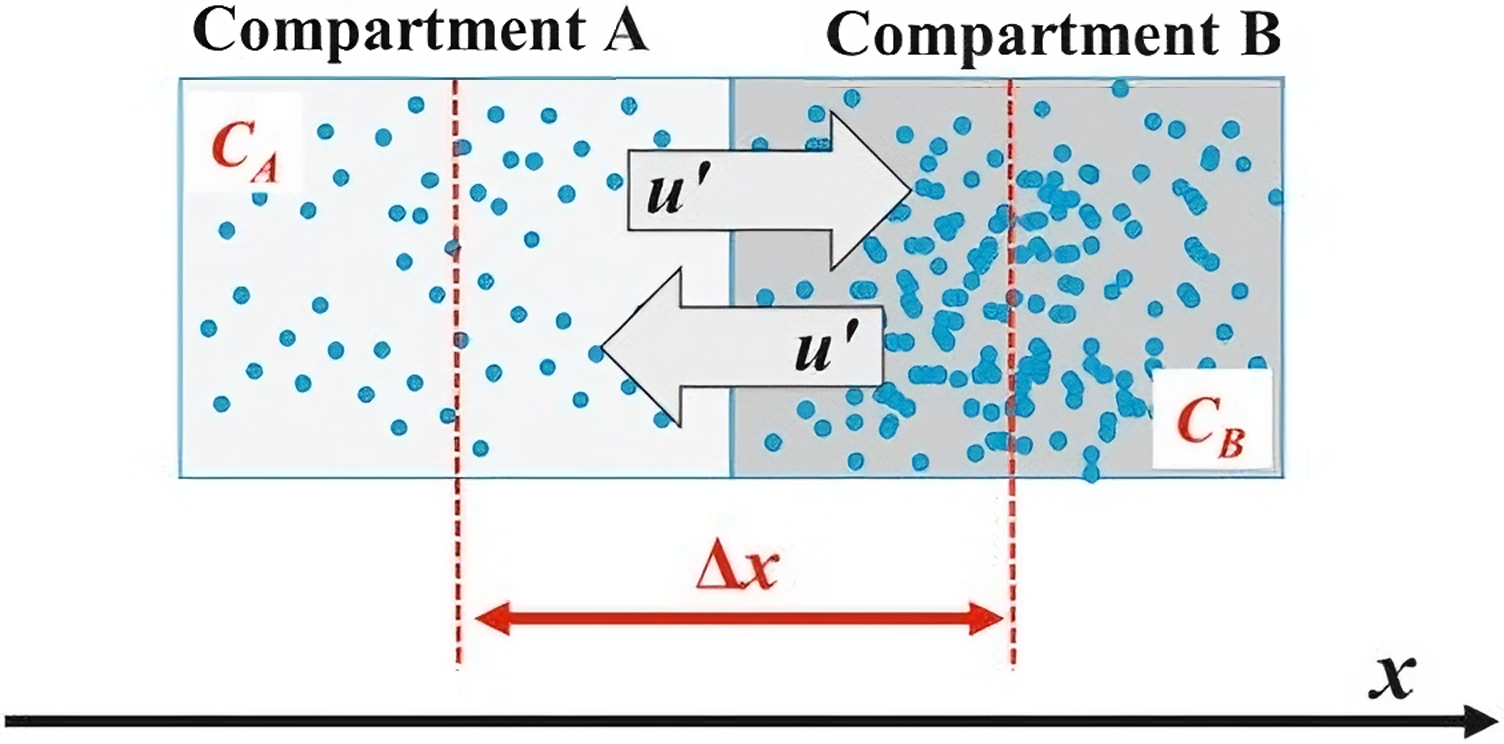
\includegraphics[width = 0.5\textwidth]{chapter_2/diffiusion_upscaled.jpg}
    \caption[]{Diffusion driven by the difference in concentration in the two compartments.}
    \label{fig:diff_drawing}
\end{figure}
[taken by https://www.sciencedirect.com/topics/earth-and-planetary-sciences/molecular-diffusion]
The simplest diffusion processes are called “normal” (or “Fickian”) and can be modelled by the two Ficks’s laws. 
\\
The first one is:
\begin{align}
    \vec{J}=-D\vec{\nabla}C \label{eq:first_law_3d}
\end{align}
Where the vectorial flow of particle $\vec{J}$ is proportional to the gradient of the concentration with a proportionality constant “$D$”, which is called diffusion coefficient. This coefficient, in general, will depend on both the substrate and the species diffusing into it, as well as on other external parameters like temperature and pressure. 
\\
It is very common to model diffusion processes one dimensionally, the first Fick’s law then becomes:
\begin{align}
    J=-D\frac{\partial C}{\partial x} \label{eq:first_law_1d}
\end{align}
Where we can clearly see that without any difference in concentration along x there is no flow of particles.
\\
The first law only describes the spatial dependence of the process. To also introduce the time dependency, it is necessary to also consider the second Fick’s Law, which states:
\begin{align}
   \frac{\partial C}{\partial t}=D\nabla^2C \label{eq:second_law_3d}
\end{align}
Under a 1-D approximation Equation~\ref{eq:second_law_3d} becomes:
\begin{align}
   \frac{\partial C}{\partial t}=D\frac{\partial^2C}{\partial x^2} \label{eq:second_law_1d}
\end{align}
Where the same proportionality constant D relates the concentration derivative with respect to time to its second spatial derivative.
\\
This partial differential equation can be solved by taking as boundary condition a fixed concentration $C_0$ at a certain value of $x$ (usually $x = 0$). This models a situation where a constant source of external diffusant is applied at one of the surfaces of a material.
\\
The solution of the equation, which is only valid for positive values of $x$, is:
\begin{align}
    C\left(x,t\right)=C_0\operatorname{erfc}\left(\frac{x}{2\sqrt{Dt}}\right) \label{eq:fick_solution}
\end{align}
Where $\mathrm{erfc}$ is the complementary of the error function and is defined as:
\begin{align}
   \operatorname{erfc}z=1-\frac{2}{\sqrt\pi}\int_{0}^{z}e^{-t^2}\ dt 
\end{align}

\begin{figure}[H]
    \centering
    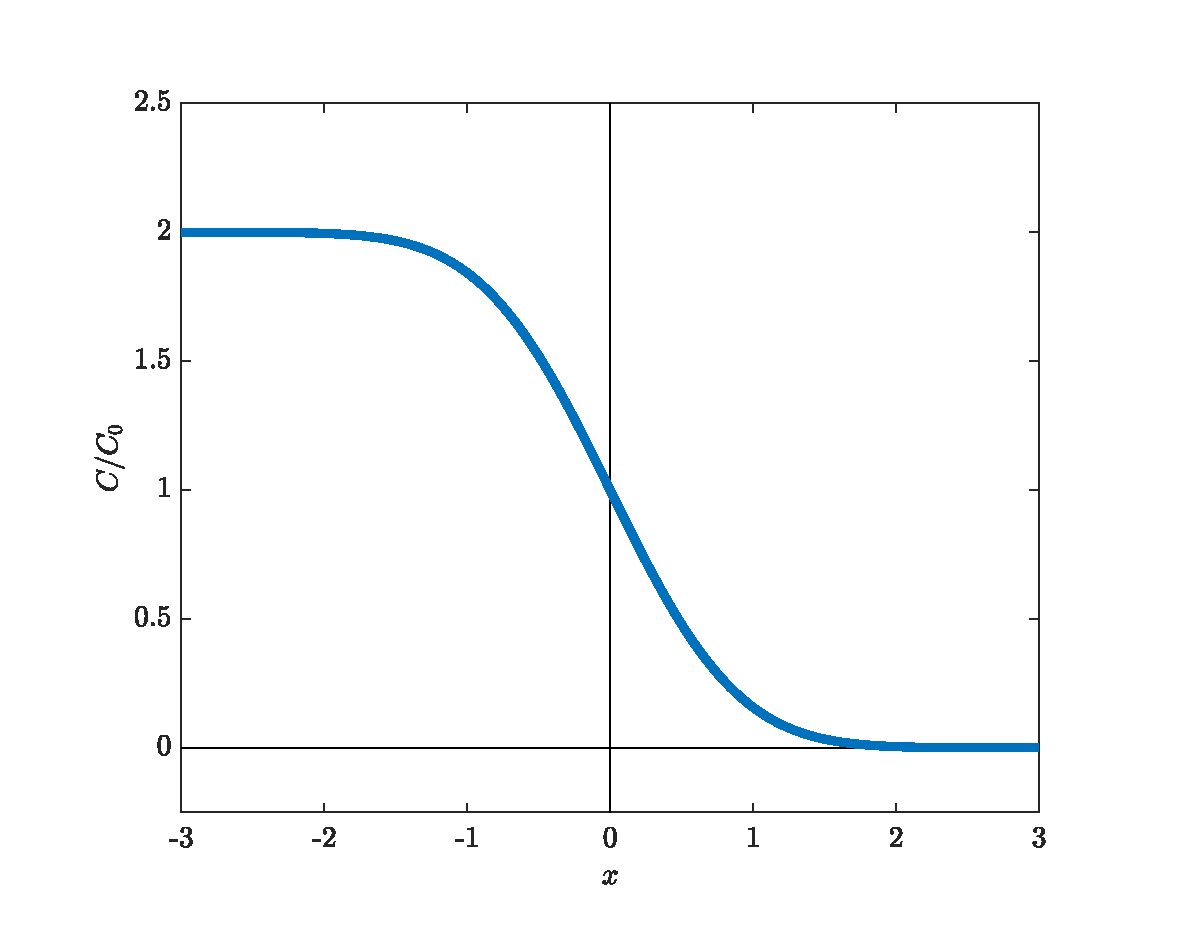
\includegraphics[width = \textwidth]{chapter_2/plot_erfc.pdf}
    \vspace*{-40pt}
    \caption[]{Plot of the complementary error function.}
    \label{fig:plot_erfc}
\end{figure}

The concentration at the source ($x = 0$) is $C_0$, in accordance with the boundary condition, decreases linearly for the region near the interface, and is followed by an exponential decay that goes to zero when we are too far from the source.


\chapter{Research Premises}
\label{ch:research_premises}
\section{Research Objectives}
After the description of the experimental apparatuses that we used, and a basic explanation of the main principles in glass polishing, we can present the main ideas and goals of the project.
\\
Due to the grinding and polishing process in optics manufacturing, contaminants can leak into the surface of the glass from both the water and the polishing suspension, possibly causing issues in the optical property of the final product.
\\
Our primary research objectives were:
\begin{enumerate}
    \item To confirm the presence of contaminants and to definitively confirm whether contamination actually occurs.
    \item To quantify the magnitude of this effect by measuring the concentration of contaminants at the surface.
    \item To investigate whether the process parameters, like polishing time or polish concentration, can have an influence on the result.
\end{enumerate}
A crucial part of our experience was to investigate whether all these evaluations could be done using a LIBS apparatus.

\section{Polishing Parameters}
\label{sec:pol_parameter}
After having thought about the parameters we could vary, we settled on a collection of variables that we identified as the most relevant:
\begin{itemize}
    \item Polishing time: by increasing the contact time we expect to see changes in the amount of concentration found at the surface.
    \item Polishing agent: expecting that the physical and chemical properties of different agents could have a different interaction with the glass. The two main polishing agents used in optics manufacturing are aluminum oxide (\ce{Al2O3}) and cerium oxide (\ce{CeO2}). The latter also usually contains traces of other elements like carbon or lanthanum.
    \item Type of water: tap water could impact the process by introducing new contaminants. Also, tap and distilled water can differ for chemical properties too, the pH of tap water is usually around 7.4 and distilled water is slightly more acidic with a pH of 5.7, due to the presence of a small amount of carbon dioxide that gets instantly dissolved into the water from the atmosphere [ph water paper].
    \item •	Polish concentration: the common concentrations used in optic manufacturing are between 5\% to 30\% in mass, where the percentage indicates the fraction of the mass of the polishing agent relative to the total weight of the slurry. Concentration influences both the mechanical properties of the solution, by physically having more particles interacting with the surface, and the chemical ones, by changing the alkalinity.
    \item Type of glass: glasses with different compositions are used in optics because their refractive index is strongly dependent on the density of the material and by introducing different and heavier elements in the glass, the manufacturer can tune its optical properties to the desired ones. Having a high concentration of different elemental species inside the glass could change the parameters that regulate diffusion at the surface.
\end{itemize}

\section{Theoretical Prediction}
\label{sec:theoretical_prediction}
As already mentioned in Chapter~\ref{sec:grinding_glass}, the description of the chemical-mechanical polishing is extremely complex, and it would be difficult to develop a model to predict and fit the results to the LIBS measurement.
\\
The simplest approach to describe the presence of contaminants in the glass is diffusion. Specifically, “normal” diffusion, where the concentration follows the two Fick’s laws. In particular, the second Fick’s law states:
\begin{align}
    C\left(x,t\right)=C_0\operatorname{erfc}\left(\frac{x}{2\sqrt{Dt}}\right) \label{eq:second_fick}
\end{align}
In the case of our LIBS measurements, we are not measuring depth resolved data. The laser ablates all the material in a small portion of the surface, and we measure the concentration of all the species that are present from the surface level to the deepest part of the ablated region. We are therefore measuring a quantity that is proportional to the integral of the concentration.
\\
Is it possible to obtain the analytical solution of the integral of the error function, by looking at some tables we find that:
\begin{align}
    \int\operatorname{erfc}\left(az\right)dz=z\operatorname{erfc}\left(az\right)-\frac{1}{a\sqrt\pi}\exp{\left(-a^2z^2\right)} \label{eq:integral_erfc}
\end{align}
In our case the parameter $a$ is equal to $\frac{1}{2\sqrt{Dt}}$. The integral is then evaluated over an interval that starts at 0, that we take as the surface level, and ends at a distance $d_a$, which is the maximum depth of the ablation. It also makes sense to normalize the expression relative to the length by dividing the integral by $d_a$.
\\
The final expression is therefore: 
 \begin{align}
    \overline{C}\left(d_{a},t\right)=C_{0}\int_{0}^{d_{a}}\operatorname{erfc}\left(\frac{x}{2\sqrt{Dt}}\right)\operatorname{d}x=C_{0}\left[d_{a}\operatorname{erfc}\left(\frac{d_{a}}{2\sqrt{Dt}}\right)-2\sqrt{\frac{Dt}{\pi}}\left[\exp\left(-\frac{d_{a}^{2}}{4Dt}\right)-1\right]\right]\frac{1}{d_a} \label{eq:c_bar_equation}
 \end{align}
There are two functional contributions to the expression:
\begin{align}
    g(t) &= d_{a\ }\operatorname{erfc}\left(\frac{d_a}{2\sqrt{Dt}}\right) \label{eq:g_t} \\
    \\[1pt]
    h(t) &= 2\sqrt{\frac{Dt}{\pi}}\left[\exp{\left(-\frac{d_a^2}{4Dt}\right)}-1\right] \label{eq:h_t}
\end{align}
In this way $\overline{C}$ can be written as $\overline{C} = g(t) + h(t)$
\\
By plotting the two contributions and the total function in a logarithmic plot, we can see that $g(t)$ and $h(t)$ intersect.
\\
The time value at the intersection point, $t_s$, separates the domain in two regions:
\begin{figure}[H]
   \centering
   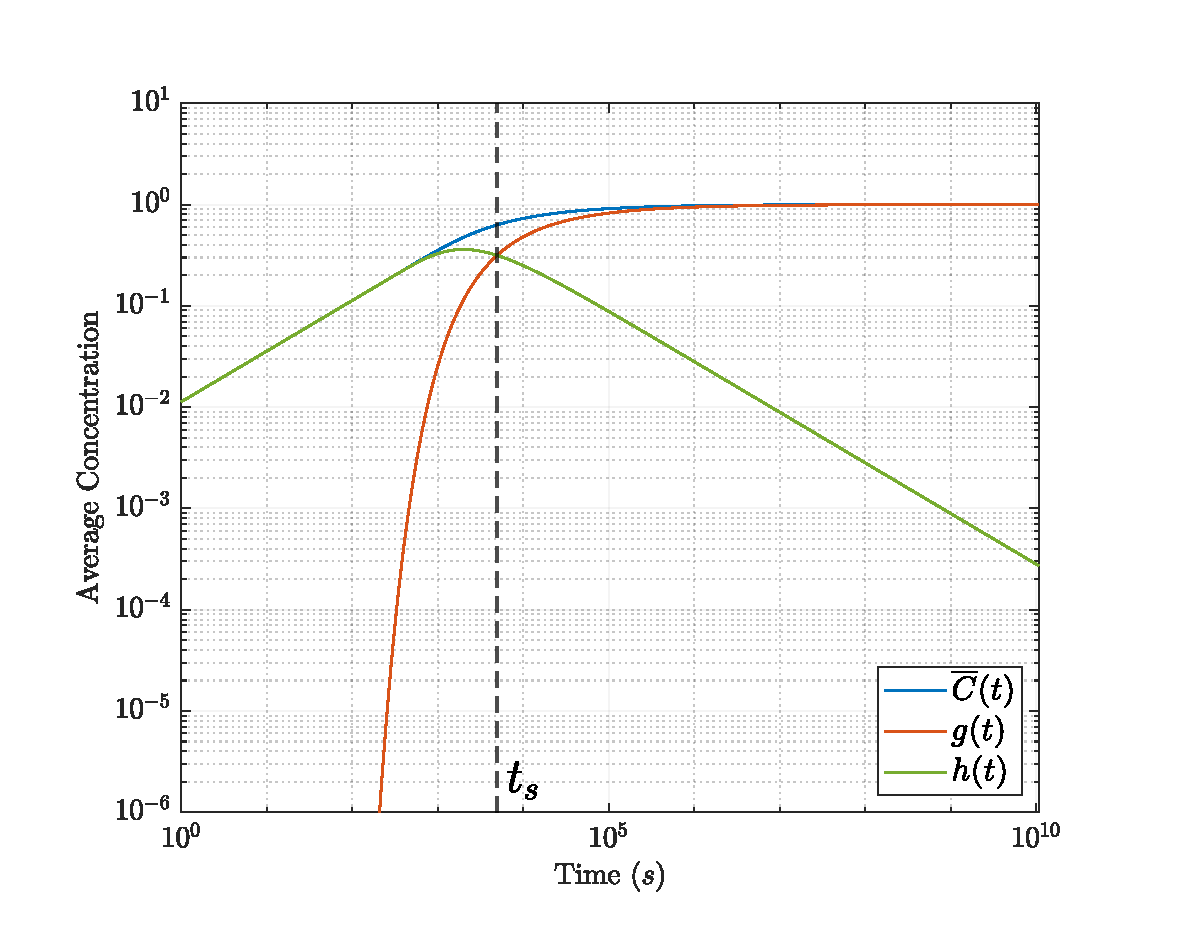
\includegraphics[width = \textwidth]{chapter_3/theoretical_cons/conc3Functions.pdf} 
   \caption{The average concentration and the two functional components. }
   \label{fig:c_bar_plot}
\end{figure}
For $t<t_s$, $h(t)$ is the dominant contribution, and the overall function behaves linearly.
\\
For $t>t_s$, $g(t)$ becomes the dominant contribution. Since $g(t)$ tends to $C_0$, $\overline{C}$ will also tend to the same parameter. Physically, this behavior represents the time values for which the saturation condition, with a homogeneous concentration equal to $C_0$, has been reached in the spatial region between 0 and $d_a$. 
\\
Considering that $D$ is always multiplying $t$, a change in the value of the diffusion coefficient, translates in a rigid shift to the left, by a value equal to $\log_{10}(D)$, of the whole function.
\\
Therefore, looking at a fixed interval of time between $t_1$ and $t_2$, two cases can be distinguished:
\\
If $t_s >> t_2$, corresponding to small values of $D$, the behavior is linear inside the considered region, and saturation is not reached.
\begin{figure}[H]
   \centering
   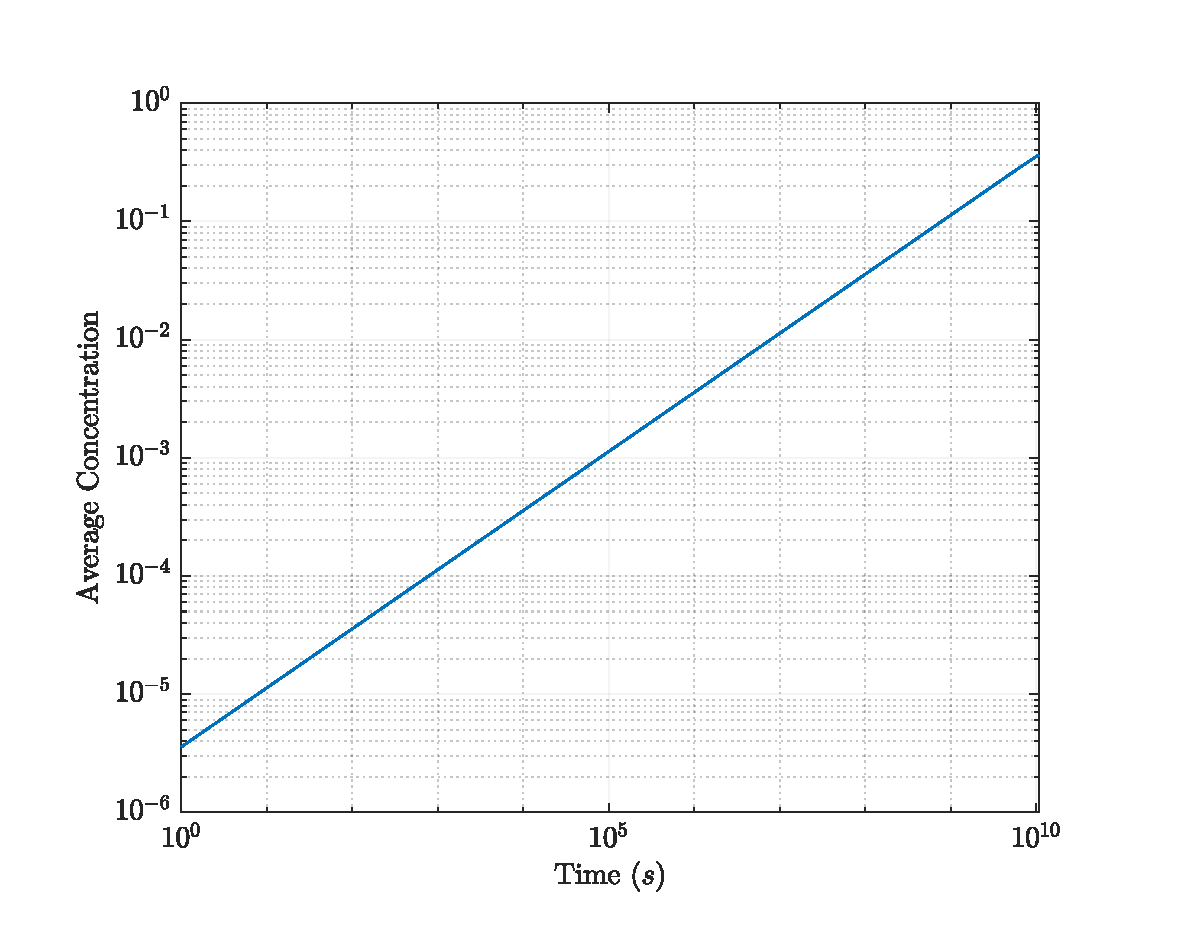
\includegraphics[width = \textwidth]{chapter_3/theoretical_cons/concRegim_linear.pdf} 
    \vspace*{-30pt}
   \caption{Linear behavior of $\bar{C}$ for $\protect t_s >> t_2$.}
   \label{fig:c_bar_linear}
\end{figure}
If $t_s ~ t_1$, corresponding to the case of a high value of $D$, saturation is reached almost instantly, and the behavior cannot be considered linear anymore.
\begin{figure}[H]
   \centering
   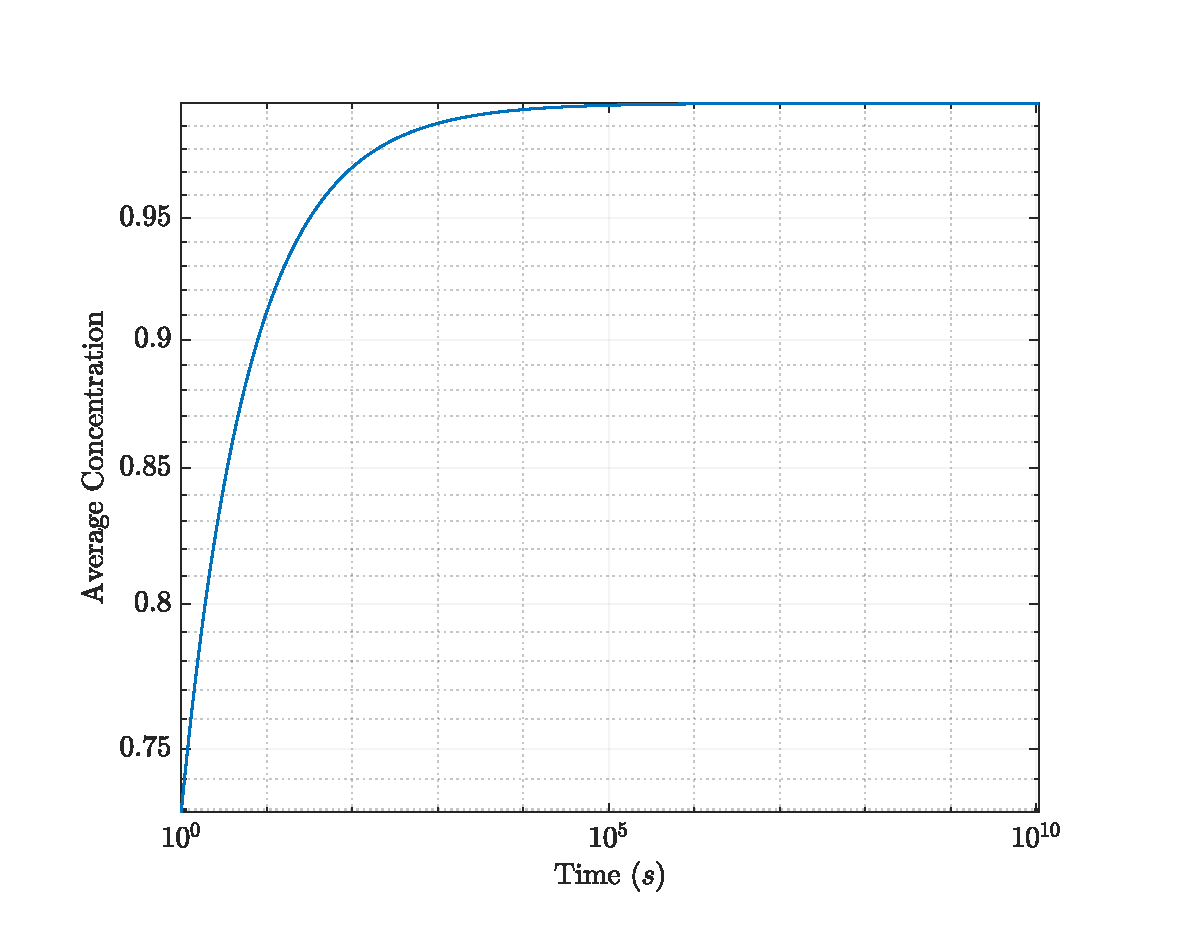
\includegraphics[width = \textwidth]{chapter_3/theoretical_cons/concRegim_exp.pdf} 
    \vspace*{-30pt}
   \caption{Non-linear behavior of $\bar{C}$ for $\protect t_s ~ t_1$.}
   \label{fig:c_bar_non_linear}
\end{figure}
If $t_s \in [t_1, t_2]$, both behaviors are present, and saturation is reached after a period of linear regime.
\begin{figure}[H]
    \centering
    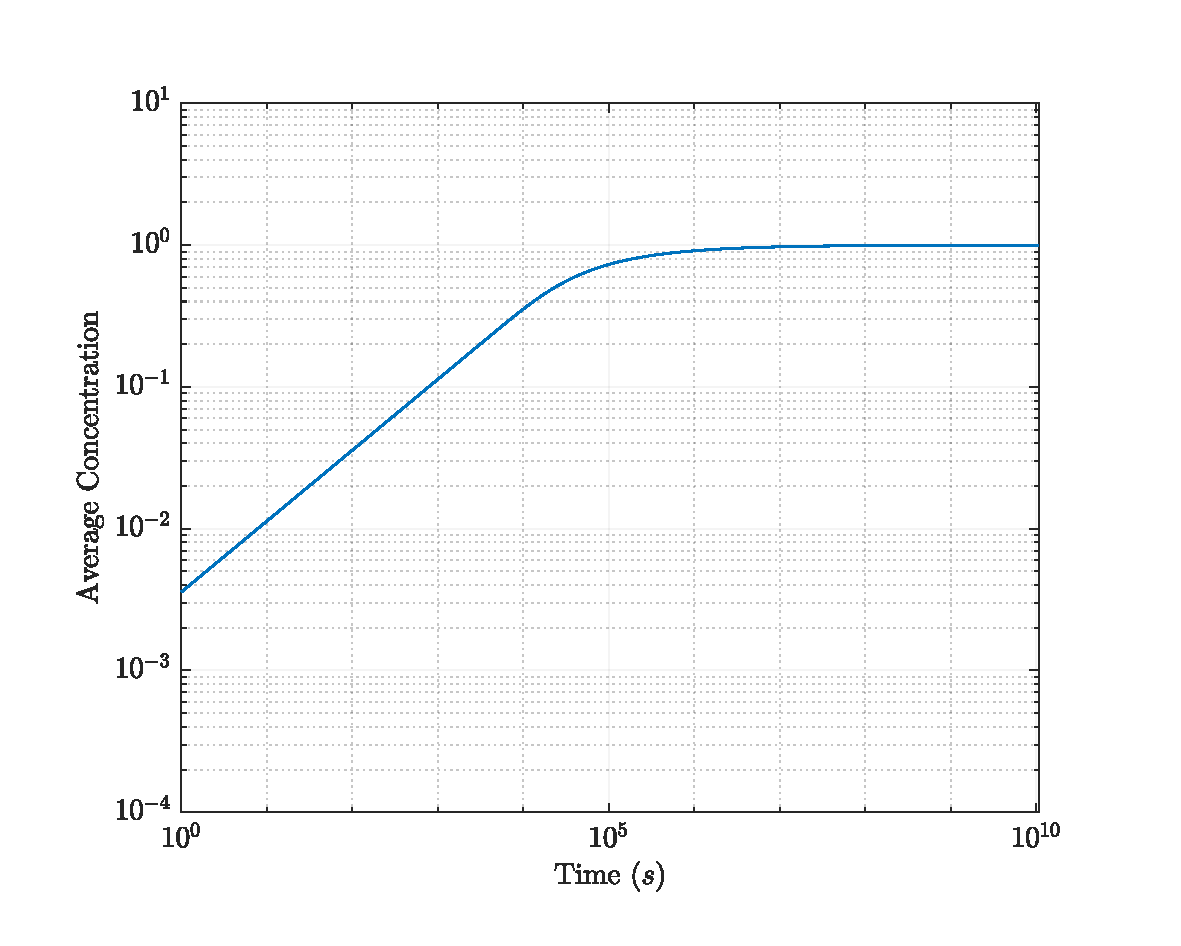
\includegraphics[width = \textwidth]{chapter_3/theoretical_cons/concRegim_mixed.pdf} 
     \vspace*{-30pt}
    \caption{General behavior of $\bar{C}$ for  $t_s \in [t_1, t_2]$.}
    \label{fig:c_bar_mixed}
 \end{figure}
This discussion is relevant because, if the predominant physical mechanism causing the presence of contaminants in the glass is actually diffusion, we should be able to estimate the value of the diffusion constant by comparing $\bar{C}$ to the data found with LIBS measurements.

\chapter{Experimental Setup}
\label{ch:experimental_setup}


\section{LIBS}
\label{sec:LIBS_apparatus}

\subsection{Description of the apparatus}
\label{sec:Description_of_the_apparatus}

As already anticipated in Chapter~\ref{sec:LIBS}, LIBS setup components are multiple.
\\
This analysis technique needs active elements capable of providing the optical energy needed for plasma formation, and a collection of optical and electronic elements capable of collecting and analyzing emitted light from the plasma.
\\
Due to the large field of application of this technique [Source of the different applications], LIBS setups are expected to vary both in size (static vs portable) and complexity.
\\
Generally, LIBS setups all share the same main elements that are listed below:
\begin{enumerate}
    \item The laser source.
    \item The optical system that focuses the laser light on the sample surface.
    \item A target holder.
    \item The light collection system, needed to convey the generated radiation to the detector.
    \item The detection system, capable of spectrally dispersing the collected light and measuring it using a digital sensor.
    \item A computer to control each previously cited element and to create the final spectrum.
\end{enumerate}
The LIBS measurements presented in this thesis have all been carried out using the same apparatus, a custom-made version of the CORALIS system by Lasertechnik Berlin with the following characteristics.

\subsubsection{Laser Source}
\label{subsubsec:laster_source}
A solid state, Nd:YAG laser source has been employed in this setup. The system gave us the possibility of tuning the laser pulse energy from less than $1 \: mJ$,  to more than 100.
\\
The Nd:YAG laser was operated at its fundamental wavelength of $1064 \: nm$ and in the Q-Switching regime, in order to achieve the high enough pulse power capable of igniting the plasma. This pulsed laser regime gives a typical duration of each pulse in the order of $5-10\: ns$ [Handbook of LIBS (other sources are possible)] and in the case of the CORALIS system the machine can provide up to 20 pulses per second, with a repetition rate of 20 Hz.

\subsubsection{Spectrometer}
\label{subsubsec:spectrometer}
The choice of the spectrometer is also dependent on the type of application and can range from the use of very simple and inexpensive components, such as line filters capable of monitoring a single predetermined wavelength, to sophisticated spectrographs allowing for the simultaneous analysis of a large spectral region.
\\
The commercially available CORALIS has only one echelle spectrometer that operates in the near-UV range (from 190 to $430 \: nm$) and has a spectral resolution that spans from 13 to $35 \: pm$, with a sensitivity of [].
\\
The modified model that we employed has an additional spectrometer that operates in the visible range (from 405 to $802\: nm$) with a spectral resolution of around $4 \: pm$, with a sensitivity of [].
[we are not sure on the value of the resolution of the Visible spectrometer, and we do not have yet the values for the sensitivity]
\\
The overall spectral region that we could analyze was therefore from 200 to $800 \: nm$.

\subsection{Parameters Chosen}
\label{subsec:parameters_chosen}
The choice of the LIBS parameters is a very crucial step in the analysis process since the quality of the results obtained from the measurements is strongly dependent on their values. In general, there are no parameters that are universally optimal, and their value changes based on the type of material, the geometry of the surface, and the element species that are being investigated.
\\
In order to arrive at the final values we employed, a thorough experimental process has been carried out.
\\
The parameters on which we had full choice were the sequent:
\begin{enumerate}
    \item Laser pulse energy.
    \item Gate width.
    \item Delay time.
    \item Detector gain.
    \item Spatial distribution of the measured points on the sample surface.
    \item Number of points per measurement.
    \item Number of laser pulses per measurement.
    \item Number of cleaning pulses before the measurement.
\end{enumerate}
The choice process for the parameters started by analyzing an NZK-7 glass sample from Schott [need the citation]. The glass sample did not undergo any post-processing phase, like grinding or polishing. From now on we will refer to this type of sample as “RAW”.
\\
The first parameter on which we focused our attention was the laser pulse energy. 
\subsubsection{Pulse Energy}
\label{subsubsec:pulse_energy}
Silica glass absorbs radiation very inefficiently in the frequency range of the laser of the apparatus we used, as it is clear from Figure~\ref{fig:glass_transmittance} at $1064 \: nm$ the glass transmittance is basically 100\%. 
\begin{figure}[H]
    \centering
    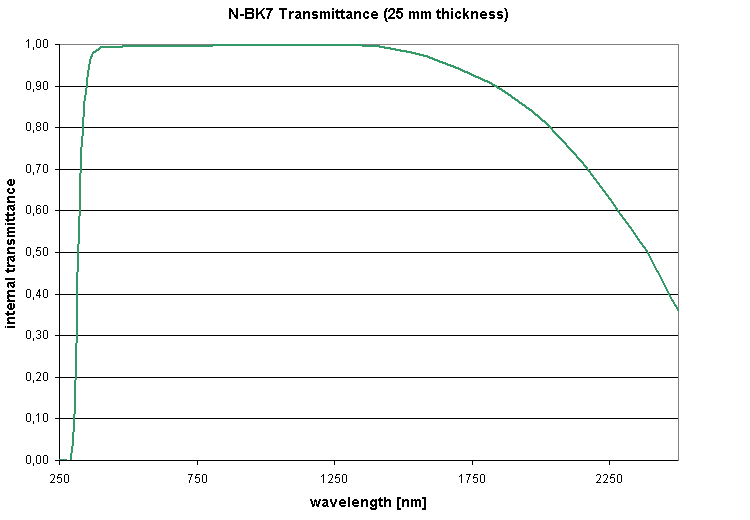
\includegraphics[width = 0.7\textwidth]{chapter_3/tests_graphs/glass_transmittance.png} 
    \caption{Transmittance of N-BK7 glass.}
    \label{fig:glass_transmittance}
 \end{figure}
 Also, in general, the lack of surface features due to polishing and grinding reduces even more the possibility of absorption. To achieve the conditions for breakdown at the surface, a high laser pulse energy must be utilized.
 \\
Tests were carried out from a lower value of $6 \:mJ$ to a higher value of $15\: mJ$.
\\
In Figure~\ref{fig:test_NZK7_6mj} and Figure~\ref{fig:test_NZK7_6mj_zoom} we can see that we already have a good spectrum even with just $6 mJ$.
\begin{figure}[H]
    \centering
    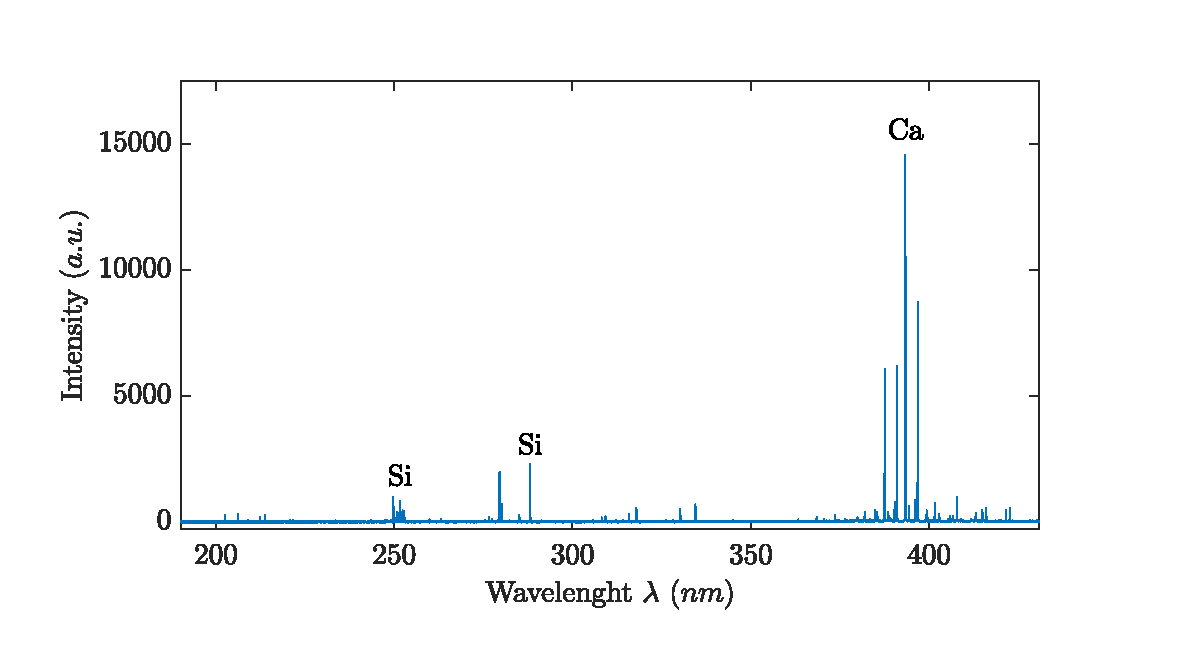
\includegraphics[width = \textwidth]{chapter_3/tests_graphs/test_NZK7_6mj.pdf} 
     \vspace*{-30pt}
    \caption{$\protect 6 \: mJ$ - Spectrum of NZK-7 glass.}
    \label{fig:test_NZK7_6mj}
\end{figure}
\begin{figure}[H]
    \centering
    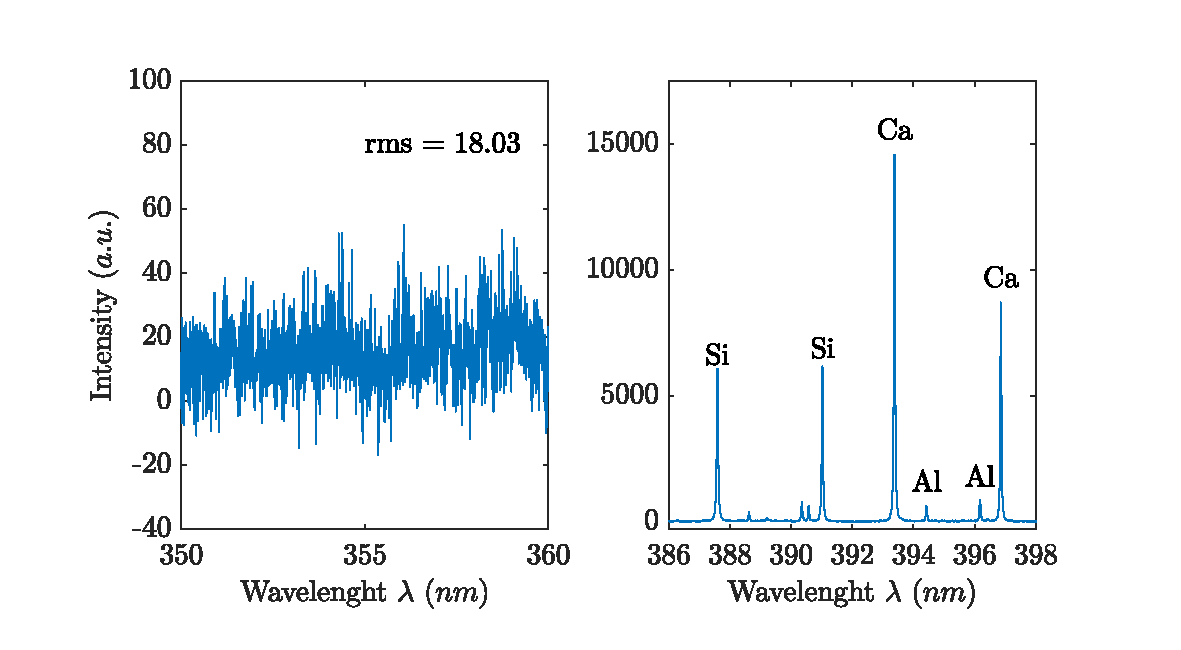
\includegraphics[width = \textwidth]{chapter_3/tests_graphs/test_NZK7_6mj_zoom.pdf} 
     \vspace*{-30pt}
    \caption{$\protect 6 \: mJ$ - (Left) Focus of on the noise. (Right) Focus on the $386 \: nm$ to $398 \: nm$ range.}
    \label{fig:test_NZK7_6mj_zoom}
 \end{figure}
Focusing on the part of the UV spectral range from $386 \: nm$ to $398 \: nm$, we see that the signal-to-noise ratio ($S.N.R$) is about 340 (the value is obtained by dividing the counts of the silicon I peak at $390.55 \: nm$ by the RMS of the noise calculated from $350 \: nm$ to $360 \: nm$).
\\
By increasing the energy value to $10 \: mJ$ we get:
\begin{figure}[H]
    \centering
    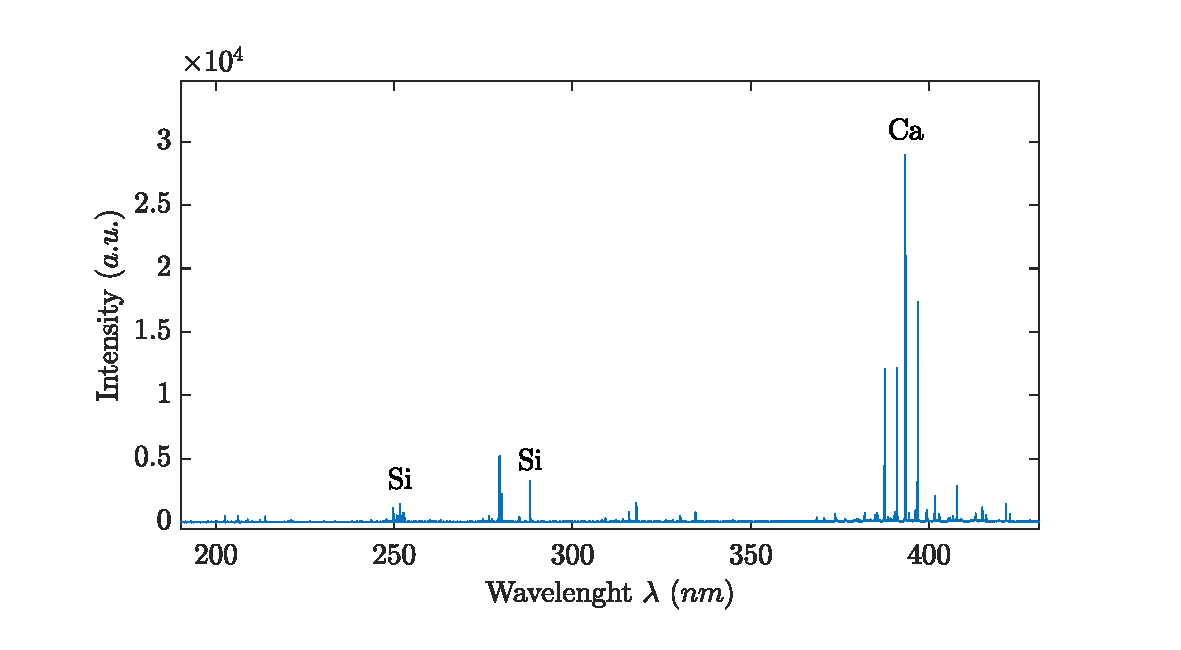
\includegraphics[width = \textwidth]{chapter_3/tests_graphs/test_NZK7_10mj.pdf} 
     \vspace*{-30pt}
    \caption{$\protect 10 \: mJ$ - Spectrum of NZK-7 glass.}
    \label{fig:test_NZK7_10mj}
\end{figure}
\begin{figure}[H]
    \centering
    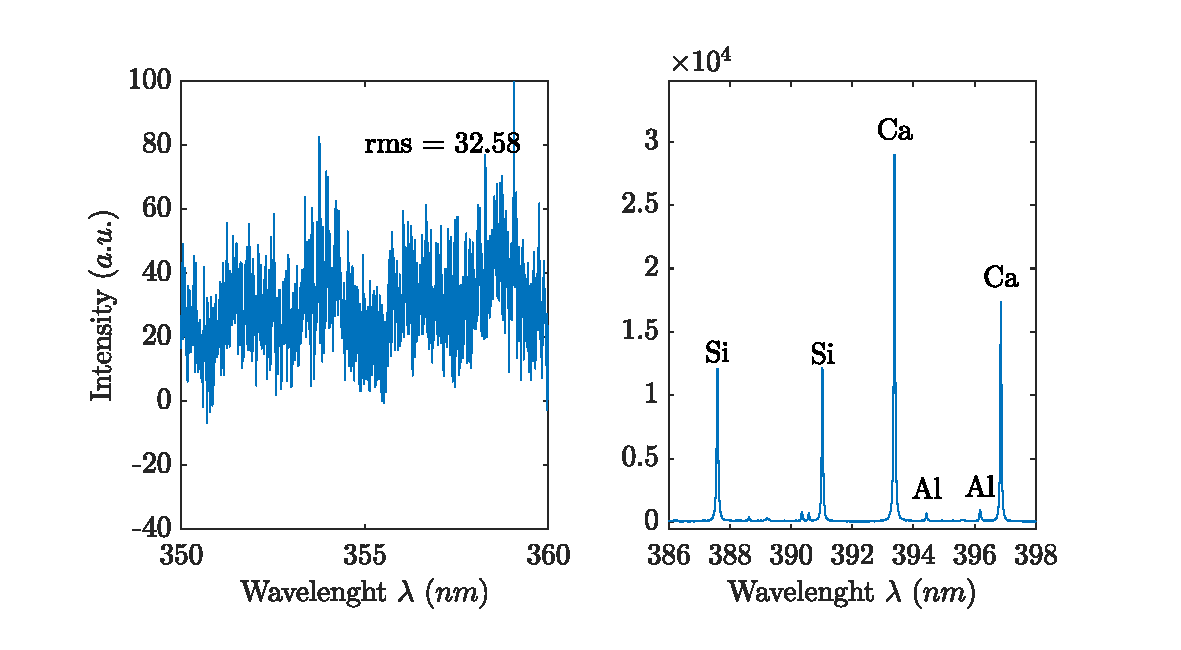
\includegraphics[width = \textwidth]{chapter_3/tests_graphs/test_NZK7_10mj_zoom.pdf} 
     \vspace*{-30pt}
    \caption{$\protect 10 \: mJ$ - (Left) Focus of on the noise. (Right) Focus on the $386 \: nm$ to $398 \: nm$ range.}
    \label{fig:test_NZK7_10mj_zoom}
 \end{figure}
Both the counts and the noise increased with the energy, but the overall $S.N.R.$ is higher, being around 370.
\\
Lastly, we tried $15 \: mJ$:
\begin{figure}[H]
    \centering
    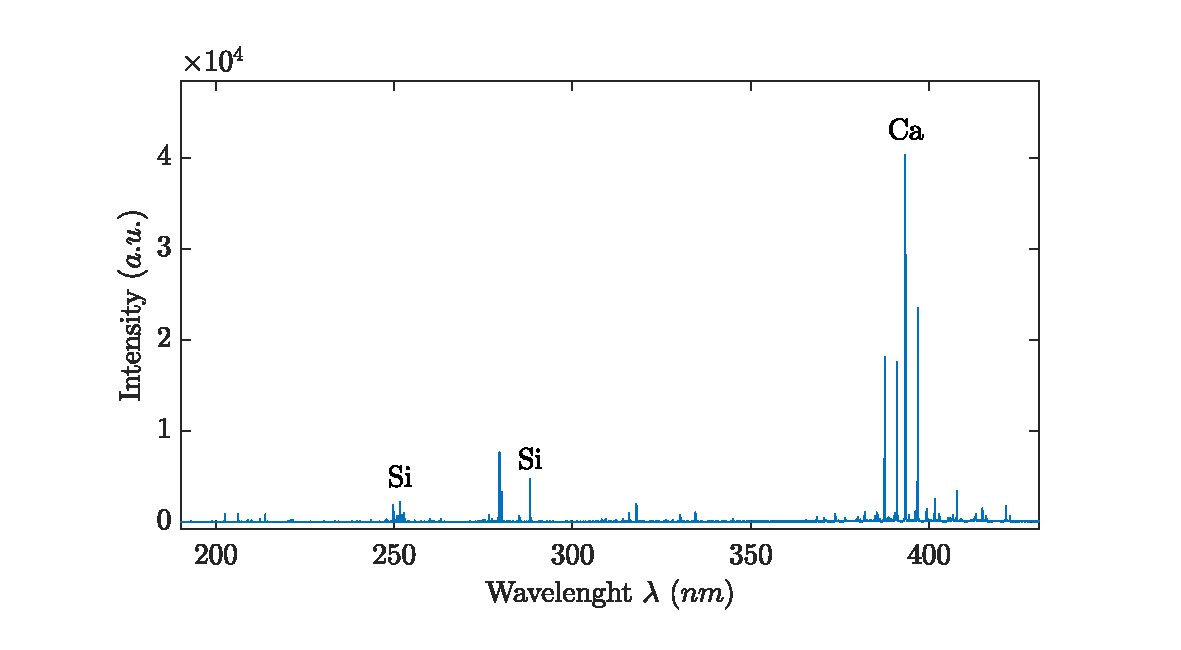
\includegraphics[width = \textwidth]{chapter_3/tests_graphs/test_NZK7_15mj.pdf} 
     \vspace*{-30pt}
    \caption{$\protect 15 \: mJ$ - Spectrum of NZK-7 glass.}
    \label{fig:test_NZK7_15mj}
\end{figure}
\begin{figure}[H]
    \centering
    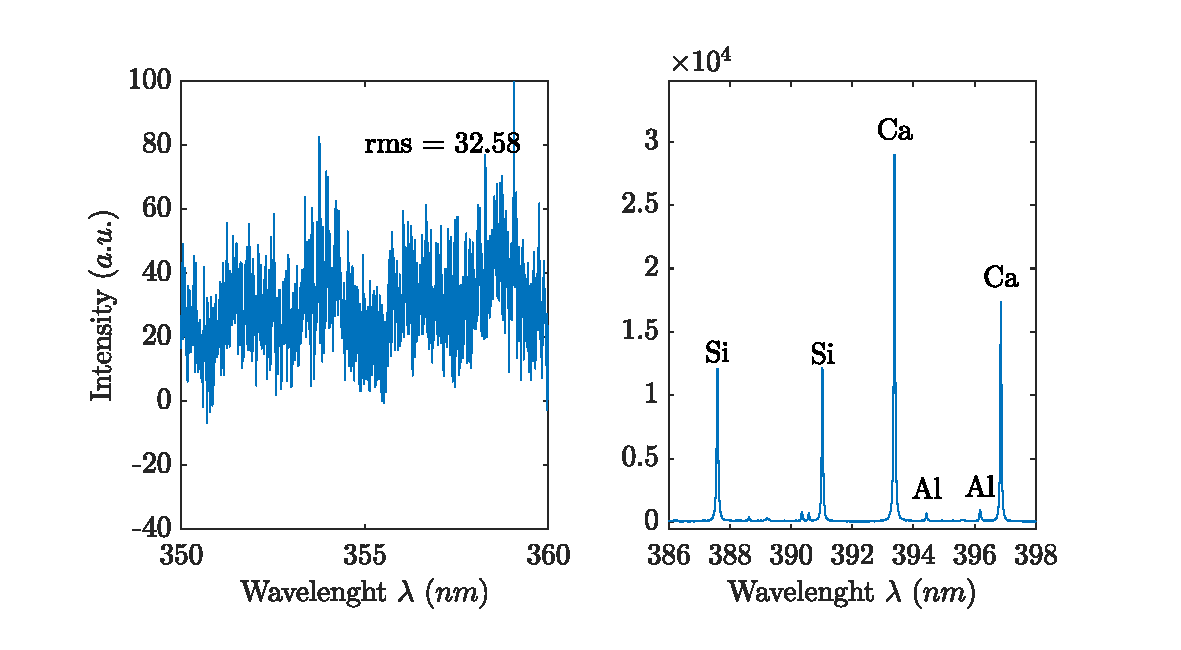
\includegraphics[width = \textwidth]{chapter_3/tests_graphs/test_NZK7_10mj_zoom.pdf} 
     \vspace*{-30pt}
    \caption{$\protect 15 \: mJ$ - (Left) Focus of on the noise. (Right) Focus on the $386 \: nm$ to $398 \: nm$ range.}
    \label{fig:test_NZK7_15mj_zoom}
 \end{figure}

For this value of the energy the $S.N.R.$ is still around 370, so we decided not to increase the energy anymore.
\\
In the end, therefore, we selected $15 \: mJ$ as the final value with which all the measurements have been carried out. 

\subsubsection{Gate Width and Time Delay}
\label{subsubsec:gate_width_delay}

To get the values that will give us the most comprehensive plasma spectrum, we decided to perform an analysis called “time evolution”, where the emission spectrum is recorded at various instants in the lifetime of the plasma. To ensure that the plasma parameters, such as electron density ($N_e$) and temperature ($T$), do not vary much within the measurements, in time evolution experiments, the gate width is always set to be equal to half the value of the time delay [jorg’s paper].
\\
The evolution was considered starting from a delay time of $0.5\: \mu s$, that corresponds to a gate width of $0.25 \: \mu s$, to a delay of $10 \: \mu s$ and $5 \: \mu s$ for the gate width.
\\
In Figure~\ref{fig:test_NZK7_time_evo_zoom} we have plotted the intensities of two silicon peaks in two different part of the spectral region for every spectrum of the time evolution. This was done to ensure that the differences measured were homogeneous along the whole frequency range.
\begin{figure}[H]
    \centering
    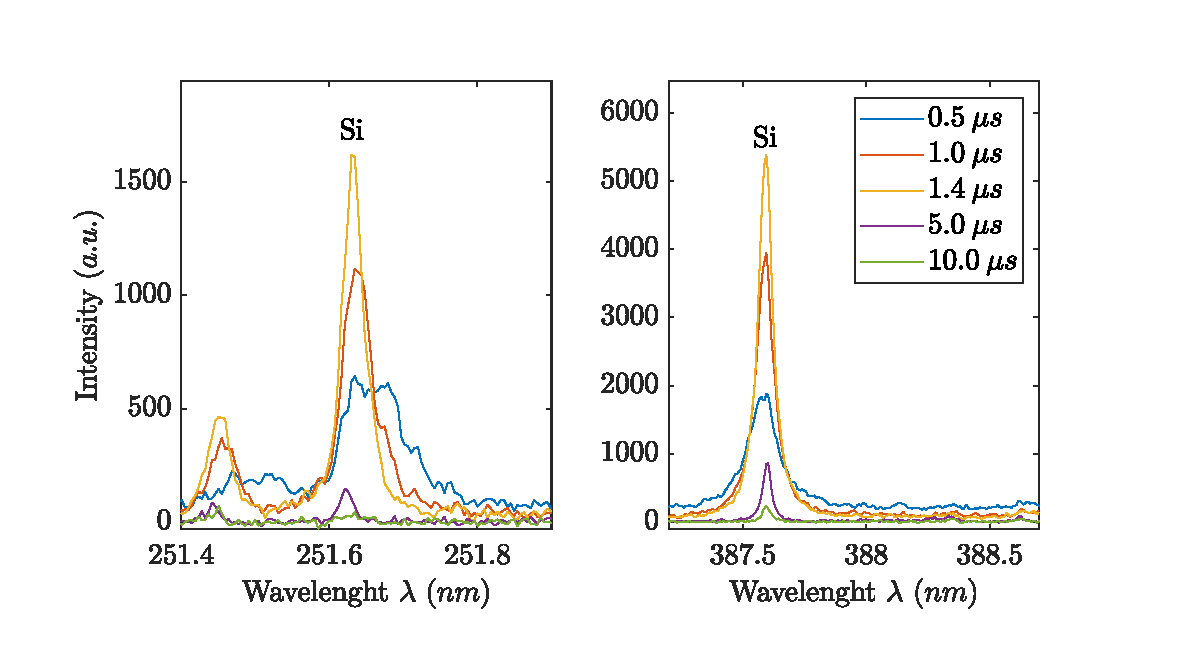
\includegraphics[width = \textwidth]{chapter_3/tests_graphs/test_NZK7_time_evo_zoom.pdf} 
    \vspace*{-30pt}
    \caption[Time evolution.]{Time evolution from $\protect 0.5\: \mu s$ to $10 \: \mu s$. (Left) Silicon peak at $251.63 \: nm$. (Right) Silicon peak at $387.53 \: nm$.}
    \label{fig:test_NZK7_time_evo_zoom}
 \end{figure}

 \begin{figure}[H]
    \centering
    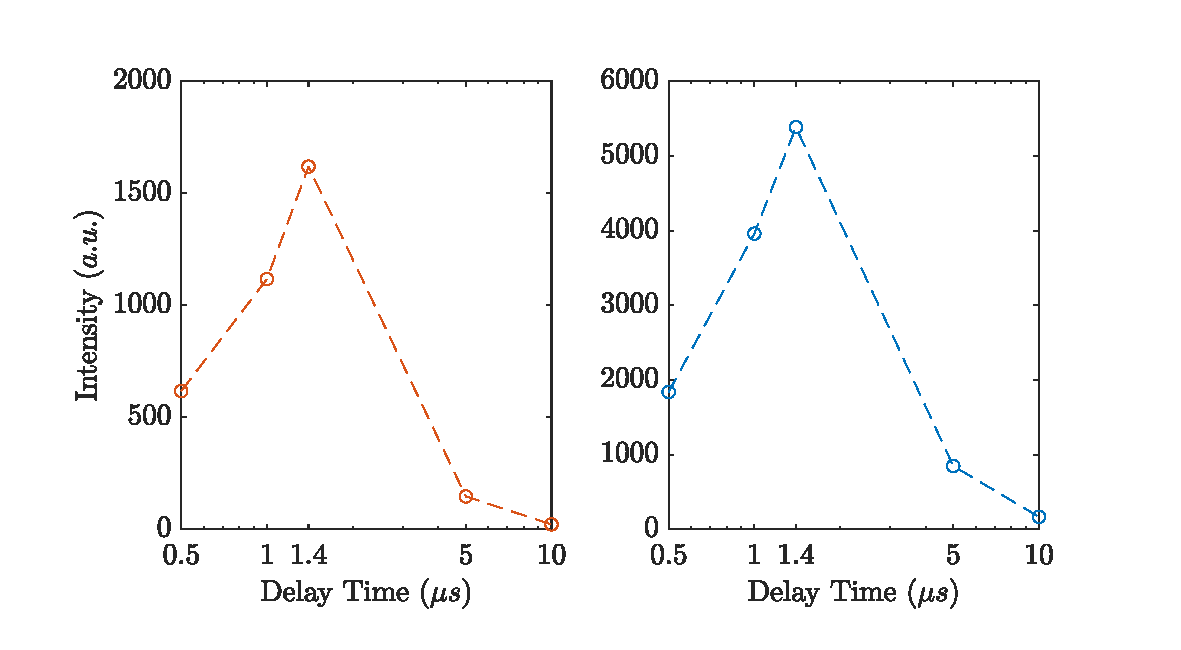
\includegraphics[width = \textwidth]{chapter_3/tests_graphs/time_evo_NZK7.pdf} 
    \vspace*{-30pt}
    \caption{Maximum intensity of the two peaks as a function of the delay time.}
    \label{fig:time_evo_NZK7}
 \end{figure}
In Figure~\ref{fig:time_evo_NZK7} is explicitly shown the maximum intensity of the two peaks as a function of the delay time. The highest intensity corresponds to a time of $1.4 \: \mu s$, and therefore this is the value that we have chosen for our measurements.
\\
Considering that the goal of our research involved finding contaminants that could be in low concentrations, for the gate width we chose a value of $12 \: \mu s$ to collect the highest amount of information possible from the measurements.

\subsubsection{Detector Gain}
\label{subsubsec:detector_gain}
The gain of the detector has been set to a value of 3000 because it is the default gain suggested by the manufacturer of the apparatus, and it is usually left unchanged.

\subsubsection{Number of Points per Measurement}
\label{subsubsec:number_points_mesurement}
Furthermore, all the analyses have been carried out taking the shots at 36 different points on the surface for each measurement. The points were separated by a distance of $150 \: \mu m$. The final spectrum is calculated as the average of the 36 different measurements, this is needed to reduce the intrinsic shot-to-shot variability that characterizes LIBS. 
\begin{figure}[H]
    \centering
    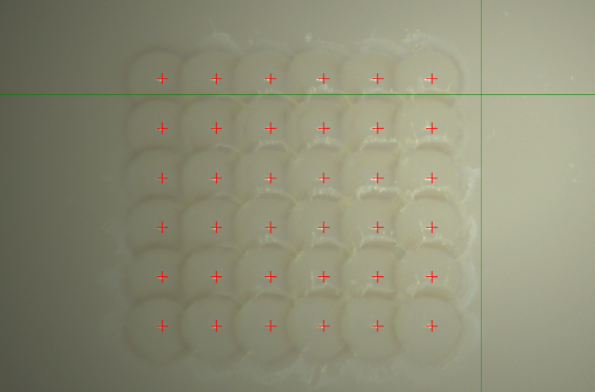
\includegraphics[width = 0.6\textwidth]{chapter_3/tests_graphs/grid_measurement.png} 
    %\vspace*{-30pt}
    \caption{Grid of measurements on the glass piece. }
    \label{fig:grid_measurement}
\end{figure}

\subsubsection{Number of Pulses per Measurement Point}
\label{subsec:number_pulses_mesurement}
Lastly, we investigated the influence on the spectrum related to the number of pulses per measurement. The LIBS apparatus gives the possibility of taking multiple laser shots at a single point on the surface, generating then the final spectrum as the average of the multiple measurements taken. This is a common way to easily increase the quality of data acquired and, usually, utilizing a large number of pulses is always preferred. The only downside in using multiple shots, other than increasing the measurement time, is that surface sensitivity is lost. In fact, each pulse ablates a portion of the material and increases the depth of the measurement.
\\ 
In our case, since contaminants are expected to diffuse only in a small region under the surface, we took a pure silica sample that had been polished for $2\:hrs$ and we took a series of consecutive measurements over the same spots to see after which number of pulses the impurities, such as aluminum, would not be detected anymore.
\\
The results are presented in Figure~\ref{fig:comparison_deep_scan}.
\begin{figure}[H]
    \centering
    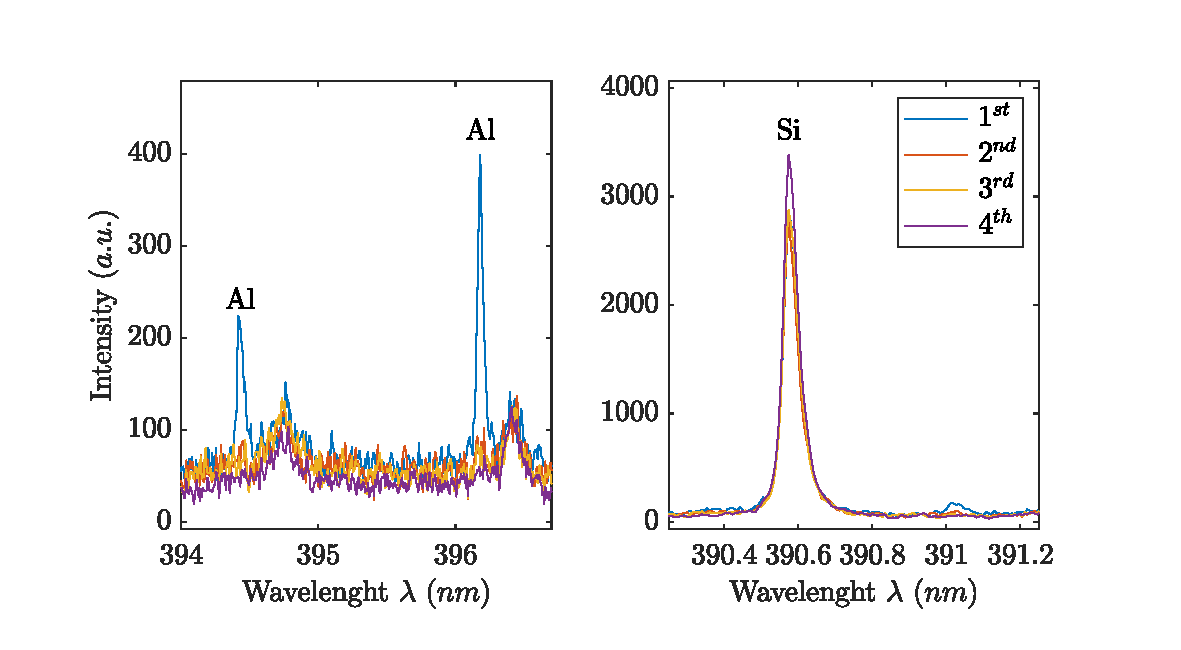
\includegraphics[width = \textwidth]{chapter_3/tests_graphs/test_NZK7_deep_scan_zoom.pdf} 
    \vspace*{-30pt}
    \caption[Comparison for consecutive pulses.]{Comparison for consecutive pulses on: (Left) Aluminum peaks around $\protect 395 \: nm$. (Right) Silicon peak at $\protect 390.6 \: nm$. The spectra are normalized with respect to the \ce{Si} peak at $\protect 288 \: nm$}
    \label{fig:comparison_deep_scan}
\end{figure}
On the left graph the most intense aluminum peaks are shown, while on the right, a nearby silicon peak is shown as a comparison. It is clear that the presence of aluminum cannot be detected after the first laser pulse, underlining its presence only on the surface. 
\\
This means that, for all our measurements, we could not perform more than one pulse. This was not ideal both for the statistical quality of the data, and for the risk of external contamination of the samples impacting on the experiment. In fact, errors in cleaning or handling of the sample, that could be averaged out by multiple pulses, could give instead a higher contribution.
\\
As a summary, the parameters chosen were:
\begin{itemize}
\item Laser energy: $15 \: mJ$
\item Delay time: $1.4 \: \mu s$
\item Gate width: $12 \: \mu s$
\item Detector gain: 3000
\item Number of pulses: 1
\end{itemize}

\subsection{Analysis Workflow}
\label{subsec:analysis_workflow}
Analysis of LIBS data is a crucial step that can be carried out both under a qualitative and a quantitative profile. Qualitative analysis requires much less time and commitment and can be carried out by a simple visual comparison of the measured spectra. It is usually employed when a fast result is needed. However, when a more sophisticated and precise result is sought, quantitative analysis can be utilized to calculate the relative concentrations of the different elemental species that compose the sample.
\\
In quantitative analyses, standard samples are usually utilized to calibrate the LIBS measurements. These are pellets prepared with well-defined and known element composition ratios.
\\
The technique that we exploited, however, is called “Calibration-free LIBS” and does not require the use of any standard for calibration. It requires instead the knowledge of some technical properties of the apparatus, as the apparatus response over the whole spectral range and the intrinsic width of the spectrometer.
\begin{figure}[H]
    \centering
    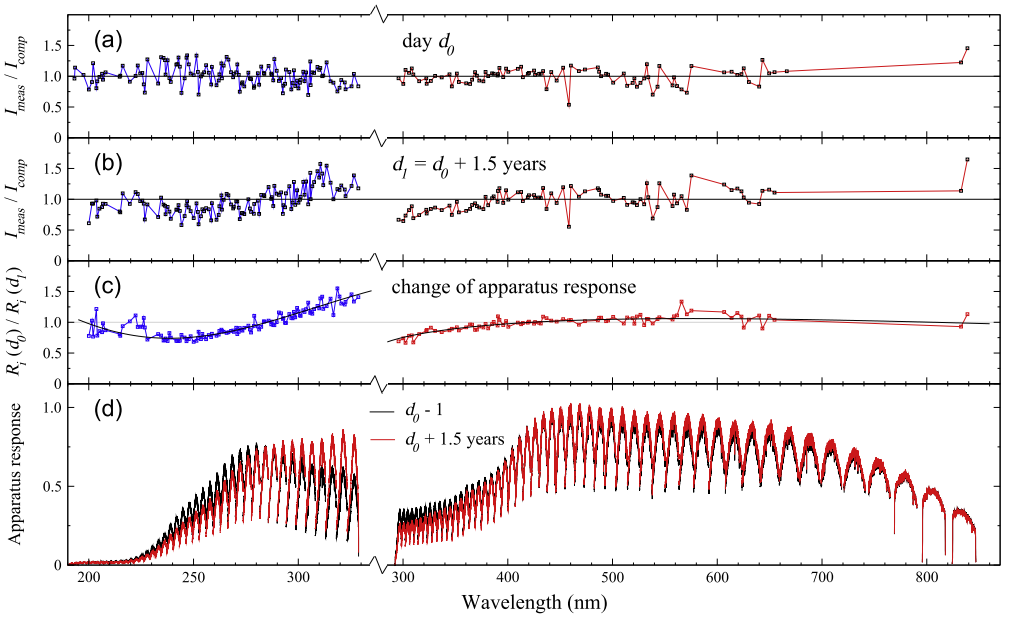
\includegraphics[width = \textwidth]{chapter_3/analysis_workflow/apparatus_response.png} 
    %\vspace*{-30pt}
    \caption{In the bottom plot of the figure it is shown an example of a typical apparatus response. }
    \label{fig:apparatus_response}
\end{figure}
In addition, for analysis to be valid, the measured plasma must satisfy the LTE condition.
\\
The analysis of the data has been carried out through the use of a program called: “Analyze LTE Plasma Spectra” (Ver. 2.6.6) or “LTEspec” in short.
\\
This application is hosted on the servers of the LP3 laboratories of the Université d’Aix-Marseille. A detailed explanation of the working principle of the algorithm behind the software can be found here [Jorg’s Paper].
\\
In the next section we will describe the passages needed to obtain the quantitative results that will be presented in the later sections.
\subsubsection{Spectra Preparation}
\label{subsubsec:spectra_preparation}
The first step is the preparation of the spectrum. The LIBS apparatus was used to measure two separate spectra, UV and visible, for each analyzed sample. To induce the exact same plasma conditions for the two ranges, we always maintained the same laser and detector parameters.


\begin{figure}[H]
    \centering
    \subfloat[UV spectrum. \label{fig:uv_non_corr}]{
        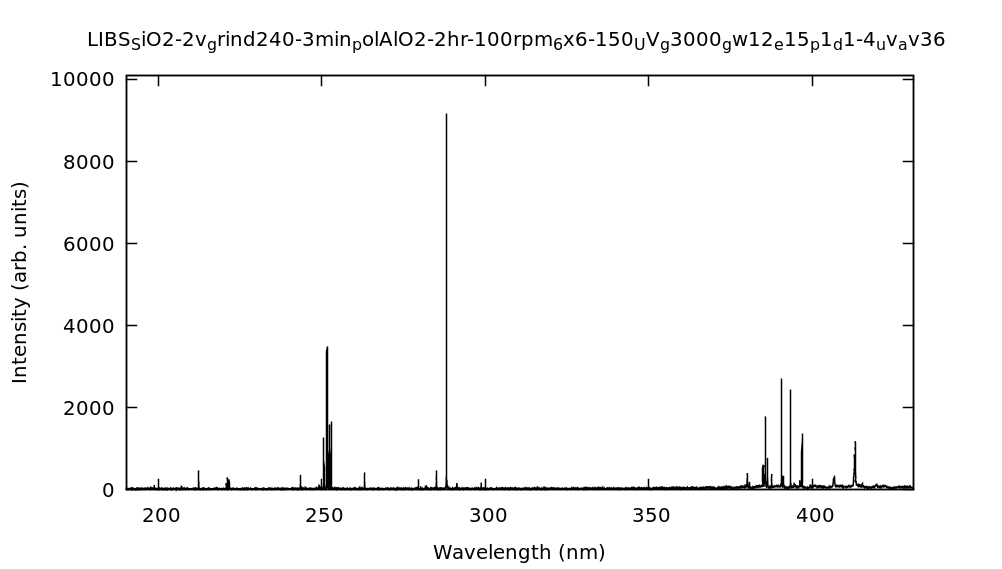
\includegraphics[width = 0.45\textwidth]{chapter_3/analysis_workflow/Uv.png}
    }
    \quad
    \subfloat[Vis Spectrum. \label{fig:vis_non_corr}]{
        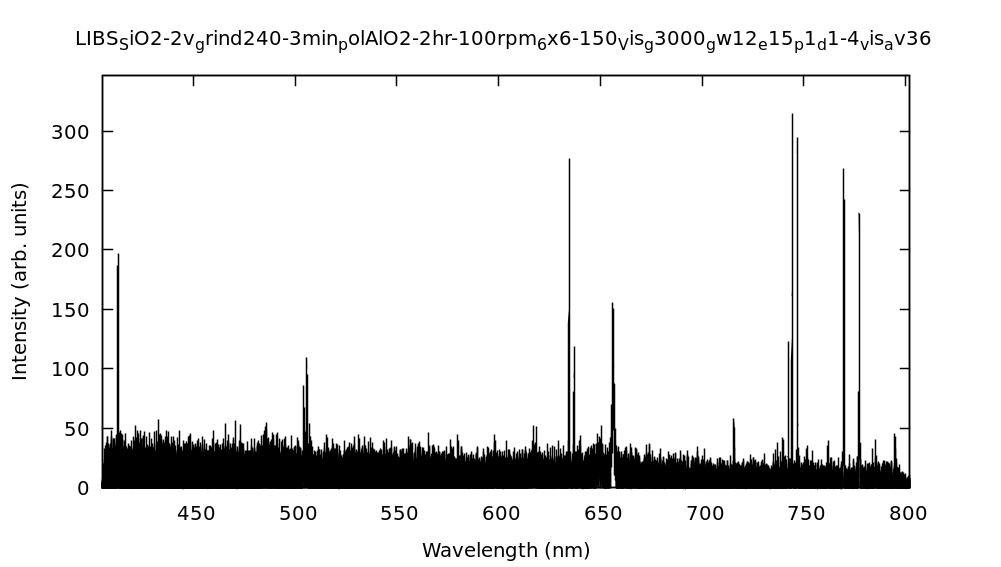
\includegraphics[width = 0.45\textwidth]{chapter_3/analysis_workflow/Vis.png}
    }
    \caption{Spectra before the correction. }
    \label{fig:spectra_before_corr}
\end{figure}




The first action we need to undertake is to connect the two graphs in order to obtain only one single spectrum comprising the whole spectral range, that spans from 190 to 800 nm. The procedure, though, is not trivial. Due to the different sensitivities of the two spectrometers, the two measured spectra have a quite different intensity reading and signal to noise ratio. In particular, the visible spectrum presents a much lower photon count.
\\ 
Thanks to the fact that the two measured spectra share a portion of the wavelength range, specifically, from 405 to 430 nm, the analysis program will use the two silicon peaks present in this region to normalize the two spectra, rescaling the intensity of the visible one. The usual rescale factor for our measurements is around 6. The visible spectrum must be therefore multiplied by 6 to match the intensities of the peaks between the UV and visible data.
\\
Here are the photos of before and after the scaling of the two spectra in the range from 400 to 430 nm, where it can be seen that the peak present at, roughly, 412 nm has been used to fit the visible (red) spectrum to the intensity of the UV (black) spectrum.


\begin{figure}[H]
    \centering
    \subfloat[UV spectrum. \label{fig:uv_vis_non_corr}]{
        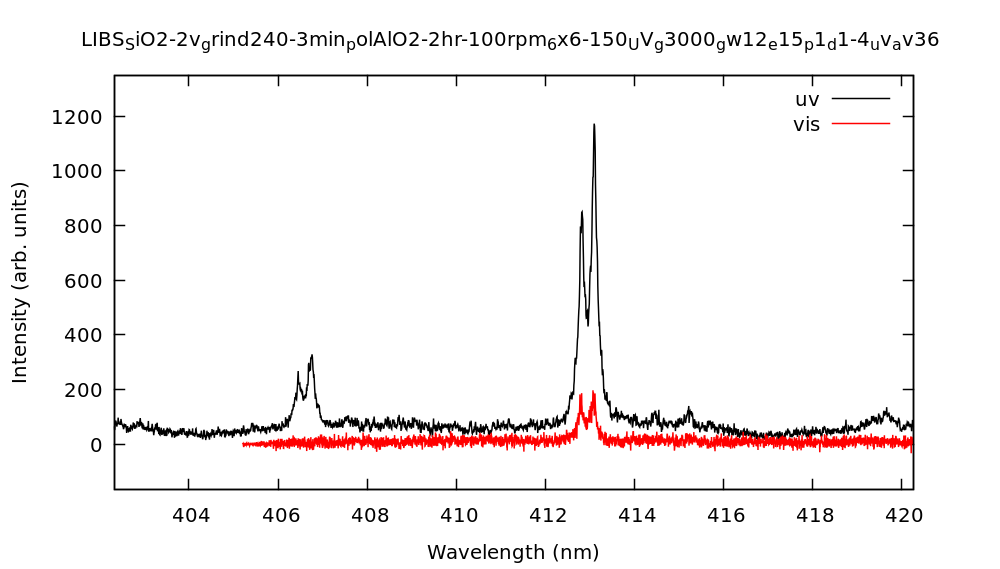
\includegraphics[width = 0.45\textwidth]{chapter_3/analysis_workflow/UvVis not corrected.png}
    }
    \quad
    \subfloat[Vis Spectrum. \label{fig:uv_vis_corr}]{
        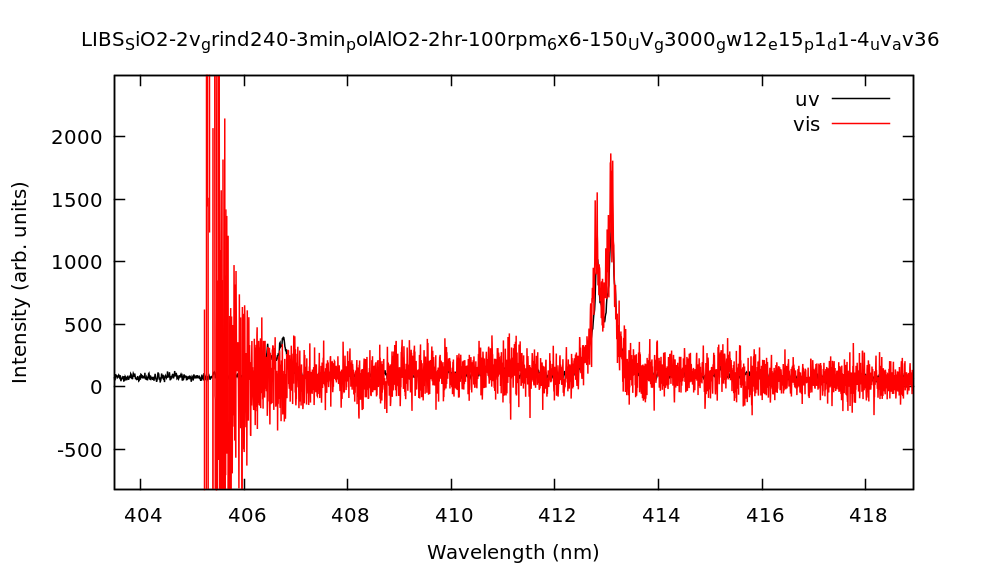
\includegraphics[width = 0.45\textwidth]{chapter_3/analysis_workflow/UvVis corrected.png}
    }
    \caption{The merging point of the two spectra before and after applying the correction and the scale factor. }
    \label{fig:spectra_mergin_point}
\end{figure}


\begin{figure}[H]
    \centering
    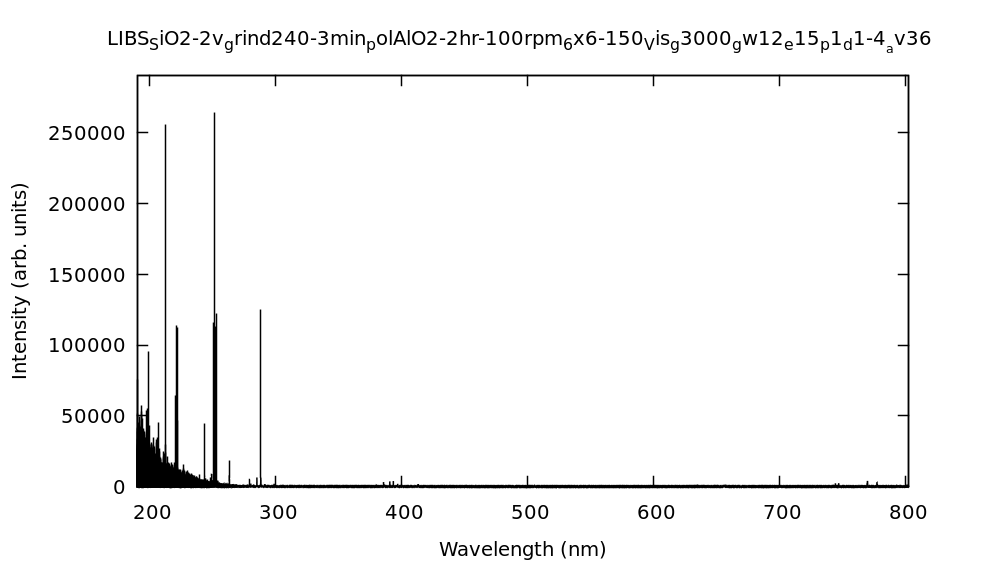
\includegraphics[width = \textwidth]{chapter_3/analysis_workflow/UvVis merged.png} 
    %\vspace*{-30pt}
    \caption{The final spectrum (UV + Vis) after the merging. }
    \label{fig:merged_sepctrum}
\end{figure}


During the merging process, the rescaling factor is not the only applied parameter. As already mentioned, the apparatus itself has a spectral response that is not homogeneous, that varies across the whole range. The spectral response had been measured, and the program can apply the corresponding correction UV and visible spectra. Lastly, other machine-dependent corrections are applied like the apparatus spectral width and the wavelength calibration are applied.

\subsubsection{Spectrum Analysis}
\label{subsubsec:spectrum_analysis}
Once the complete spectrum has been derived, the proper quantitative analysis can start. 

\paragraph{Electron density and Optical Thickness}
\label{par:electron_density_opt_thick}
The first step in the plasma diagnostic process is to select a reference intensity peak from which Stark and Doppler broadening parameters are measured; these are in fact the dominant mechanisms of spectra line broadening in laser induced plasmas [Paper’s 36][maybe cite the chapter of the thesis]. Those values are then used to measure the plasma optical thickness.
\\
Under the assumption of a linear dependance of the Stark width and shift with the electron density, the latter can be derived by measuring the width of a line with a significant Stark shift. A common choice for this estimation is the H-$\alpha$ lines at $656.28\:nm$ [Paper].
\\
In our case the Si I transition at $390.55 \: nm$ has been chosen for both the measurements.
\paragraph{Plasma Temperature}
\label{par:plasma_temperature}
After the determination of the electron density, the plasma temperature is derived from the Boltzmann plot (Chapter~\ref{subsubsec:thermodynamic_eq}) regarding the \ce{Si I} $390.55\:nm$ line and the ionized \ce{Si II} doublet at 385.60 and $386.26\:nm$ [Paper].


\begin{figure}[H]
    \centering
    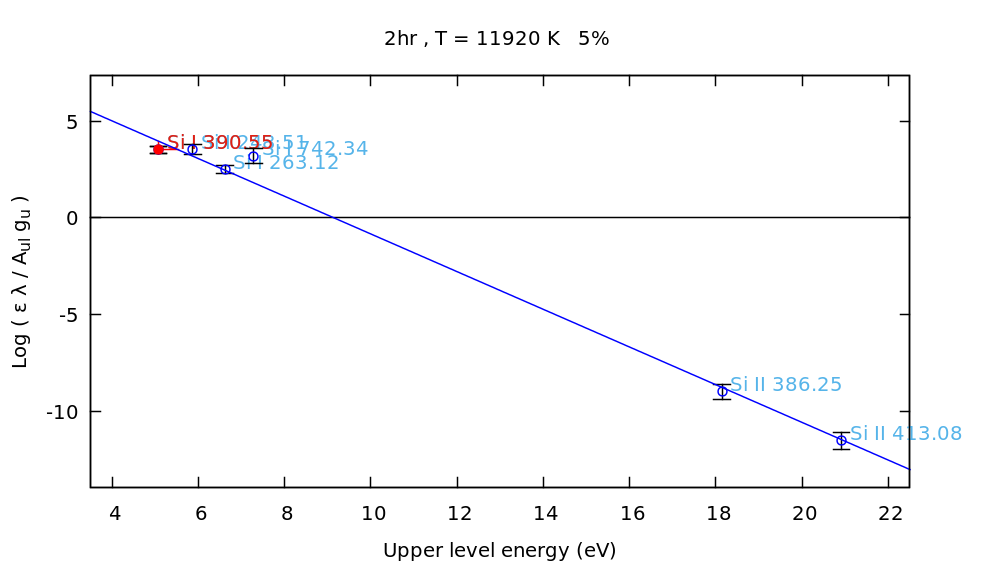
\includegraphics[width = \textwidth]{chapter_3/analysis_workflow/Boltzmann plot SI.png} 
    %\vspace*{-30pt}
    \caption{Boltzmann plot used to estimate the plasma temperature. }
    \label{fig:boltzmann_plot}
\end{figure}


\paragraph{Plasma Parameter}
\label{par:plasma_parameter}
The size of the plasma is derived from interpolating the laser settings present in the metadata of the file, with experimental measurements done at the apparatus, where the size of the plasma was measured over its whole lifetime using a high-speed camera.
\paragraph{Element Search and Relative Concentration Calculation}
Once an approximate value of the electron density Ne, the plasma temperature T and the optical thickness of the plasma have been measured, it is possible to carry out an automatic search of the element species that are present in the plasma. 
The spectral lines used for the analysis are selected according to the following criteria [Paper]:
\begin{itemize}
    \item The overlapping of spectral lines has to be avoided.
    \item The emission intensity must be large enough in order to have a large signal to noise ratio for the selected peaks.
    \item The lines must have a weak enough optical thickness to have a significant correlation between elemental concentration and line intensity
\end{itemize}

Here are presented some plots of the elements’ measured lines (in black), versus the expected emission based on the calculated plasma parameters and estimated concentration (in red). The more the fitting is precise, the more the plasma parameters represent valid approximations of the real values.

\begin{figure}[H]
    \centering
    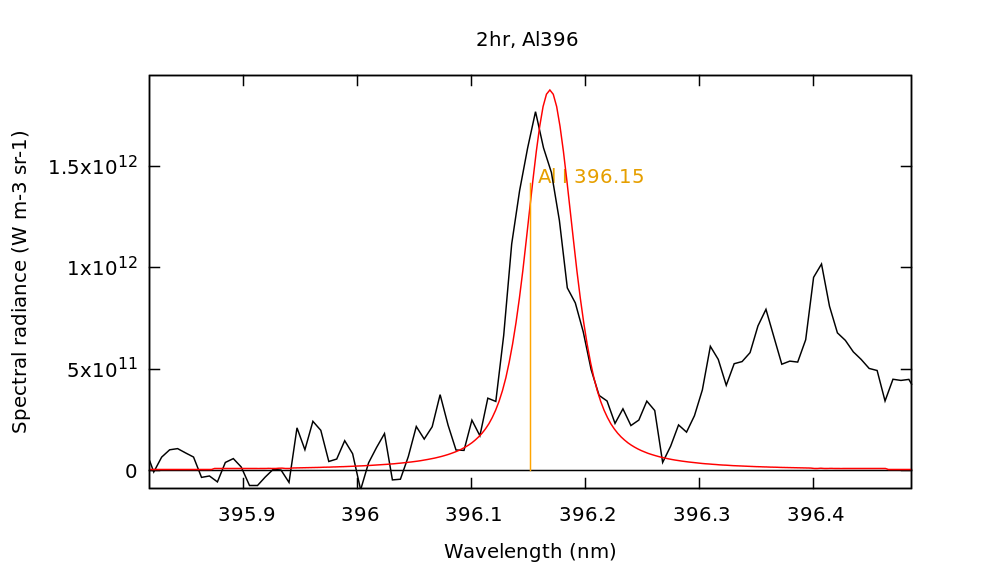
\includegraphics[width = 0.8\textwidth]{chapter_3/analysis_workflow/Al I line 396.png} 
    %\vspace*{-30pt}
    \caption{Aluminum line at $\protect 396.15 \:nm$}
    \label{fig:aluminum_line_lte}
\end{figure}
\begin{figure}[H]
    \centering
    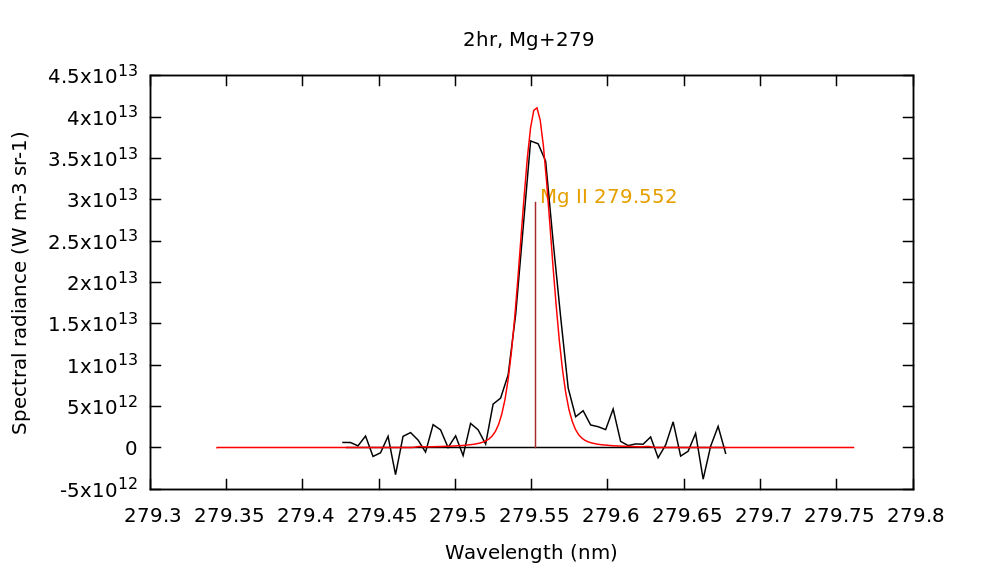
\includegraphics[width = 0.8\textwidth]{chapter_3/analysis_workflow/Mg II line 279.png} 
    %\vspace*{-30pt}
    \caption{Magnesium line at $\protect 279.55 \:nm$ }
    \label{fig:magnesium_line_lte}
\end{figure}
\begin{figure}[H]
    \centering
    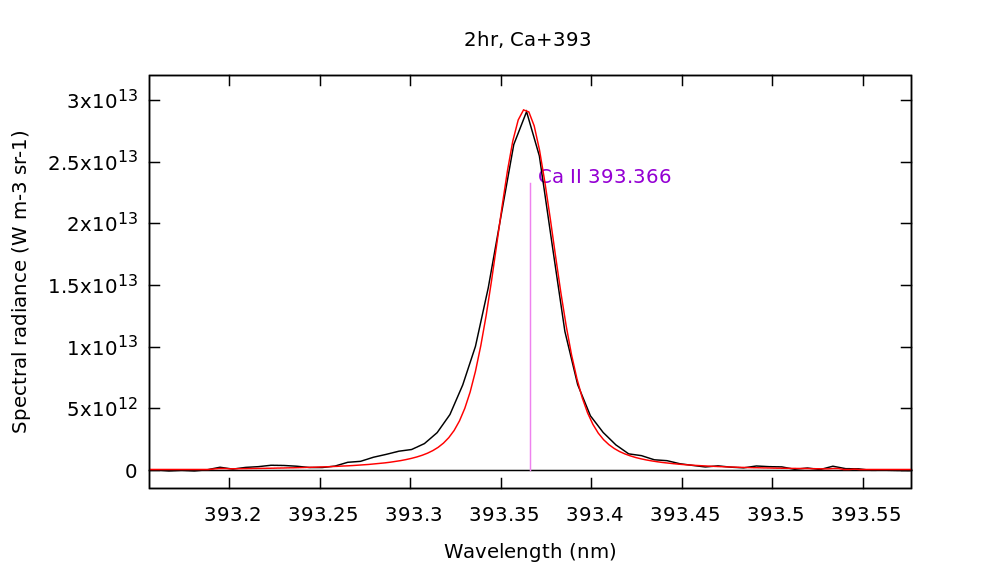
\includegraphics[width = 0.8\textwidth]{chapter_3/analysis_workflow/Ca II line 393.png} 
    %\vspace*{-30pt}
    \caption{Calcium line at $\protect 393.37 \:nm$ }
    \label{fig:calcium_line_lte}
\end{figure}

After the elements have been identified, all the plasma parameters are derived again, along with the relative concentrations of the elements. 

\subsubsection{Issues with Oxygen}
\label{subsubsec:oxygen_issues}

Particular attention must be paid with respect to the measurement of the oxygen concentration. In pure fused silica glass (\ce{SiO2}), oxygen makes up for most of the species in the glass composition, since its stoichiometric contribution is of about 2/3, or roughly 68\% of the total number of atoms. Oxygen atoms are characterized by large gaps between energy levels of the exited states, for this reason, for most the oxygen species, the thermodynamic equilibrium is hardly established [paper jorg] and therefore the measured lines cannot be use in the calibration-free method.
\\
This issue is even more noticeable when carrying out LIBS measurements in ambient air, like in our case, because oxygen is also present in the air surrounding the target sample and therefore, the measured emission is higher relative to the expected one from the real composition of the sample. 
\\
Under this condition, the standard procedure is to manually set the relative concentration of oxygen to be equal to the theoretical stoichiometric fraction. For our purposes, the concentration of oxygen is not a relevant quantity and therefore this approximation should not impact the other measurements.













\section{Polishing}
\label{Polishing}
Ensuring a uniform and correct polishing of the glass samples was one of the main concerns of our project. The procedure had to be reproducible and consistent between different runs, in order to introduce the least amount of non-controllable variables and to isolate the effect of the parameters that we were investigating.
\\
In addition, some of the samples were processed even up to consecutive hours, so a partial automatization of the workflow had to be done.
\subsection{Description of the Polishing Apparatus}
\label{subsec:description_polish_apparatus}
In this section, we will briefly describe the primary instrumentation we employed for glass processing.

\subsubsection{Polishing Machine}
\label{subsubsec:polishing_machine}
The polishing machine is one of the most important components.
\\
For our purposes, we employed a model manufactured by the company Buehler, specifically the Ecomet 4. The machine was utilized both to grind and polish all the analyzed glass samples. 
\begin{figure}[H]
    \centering
    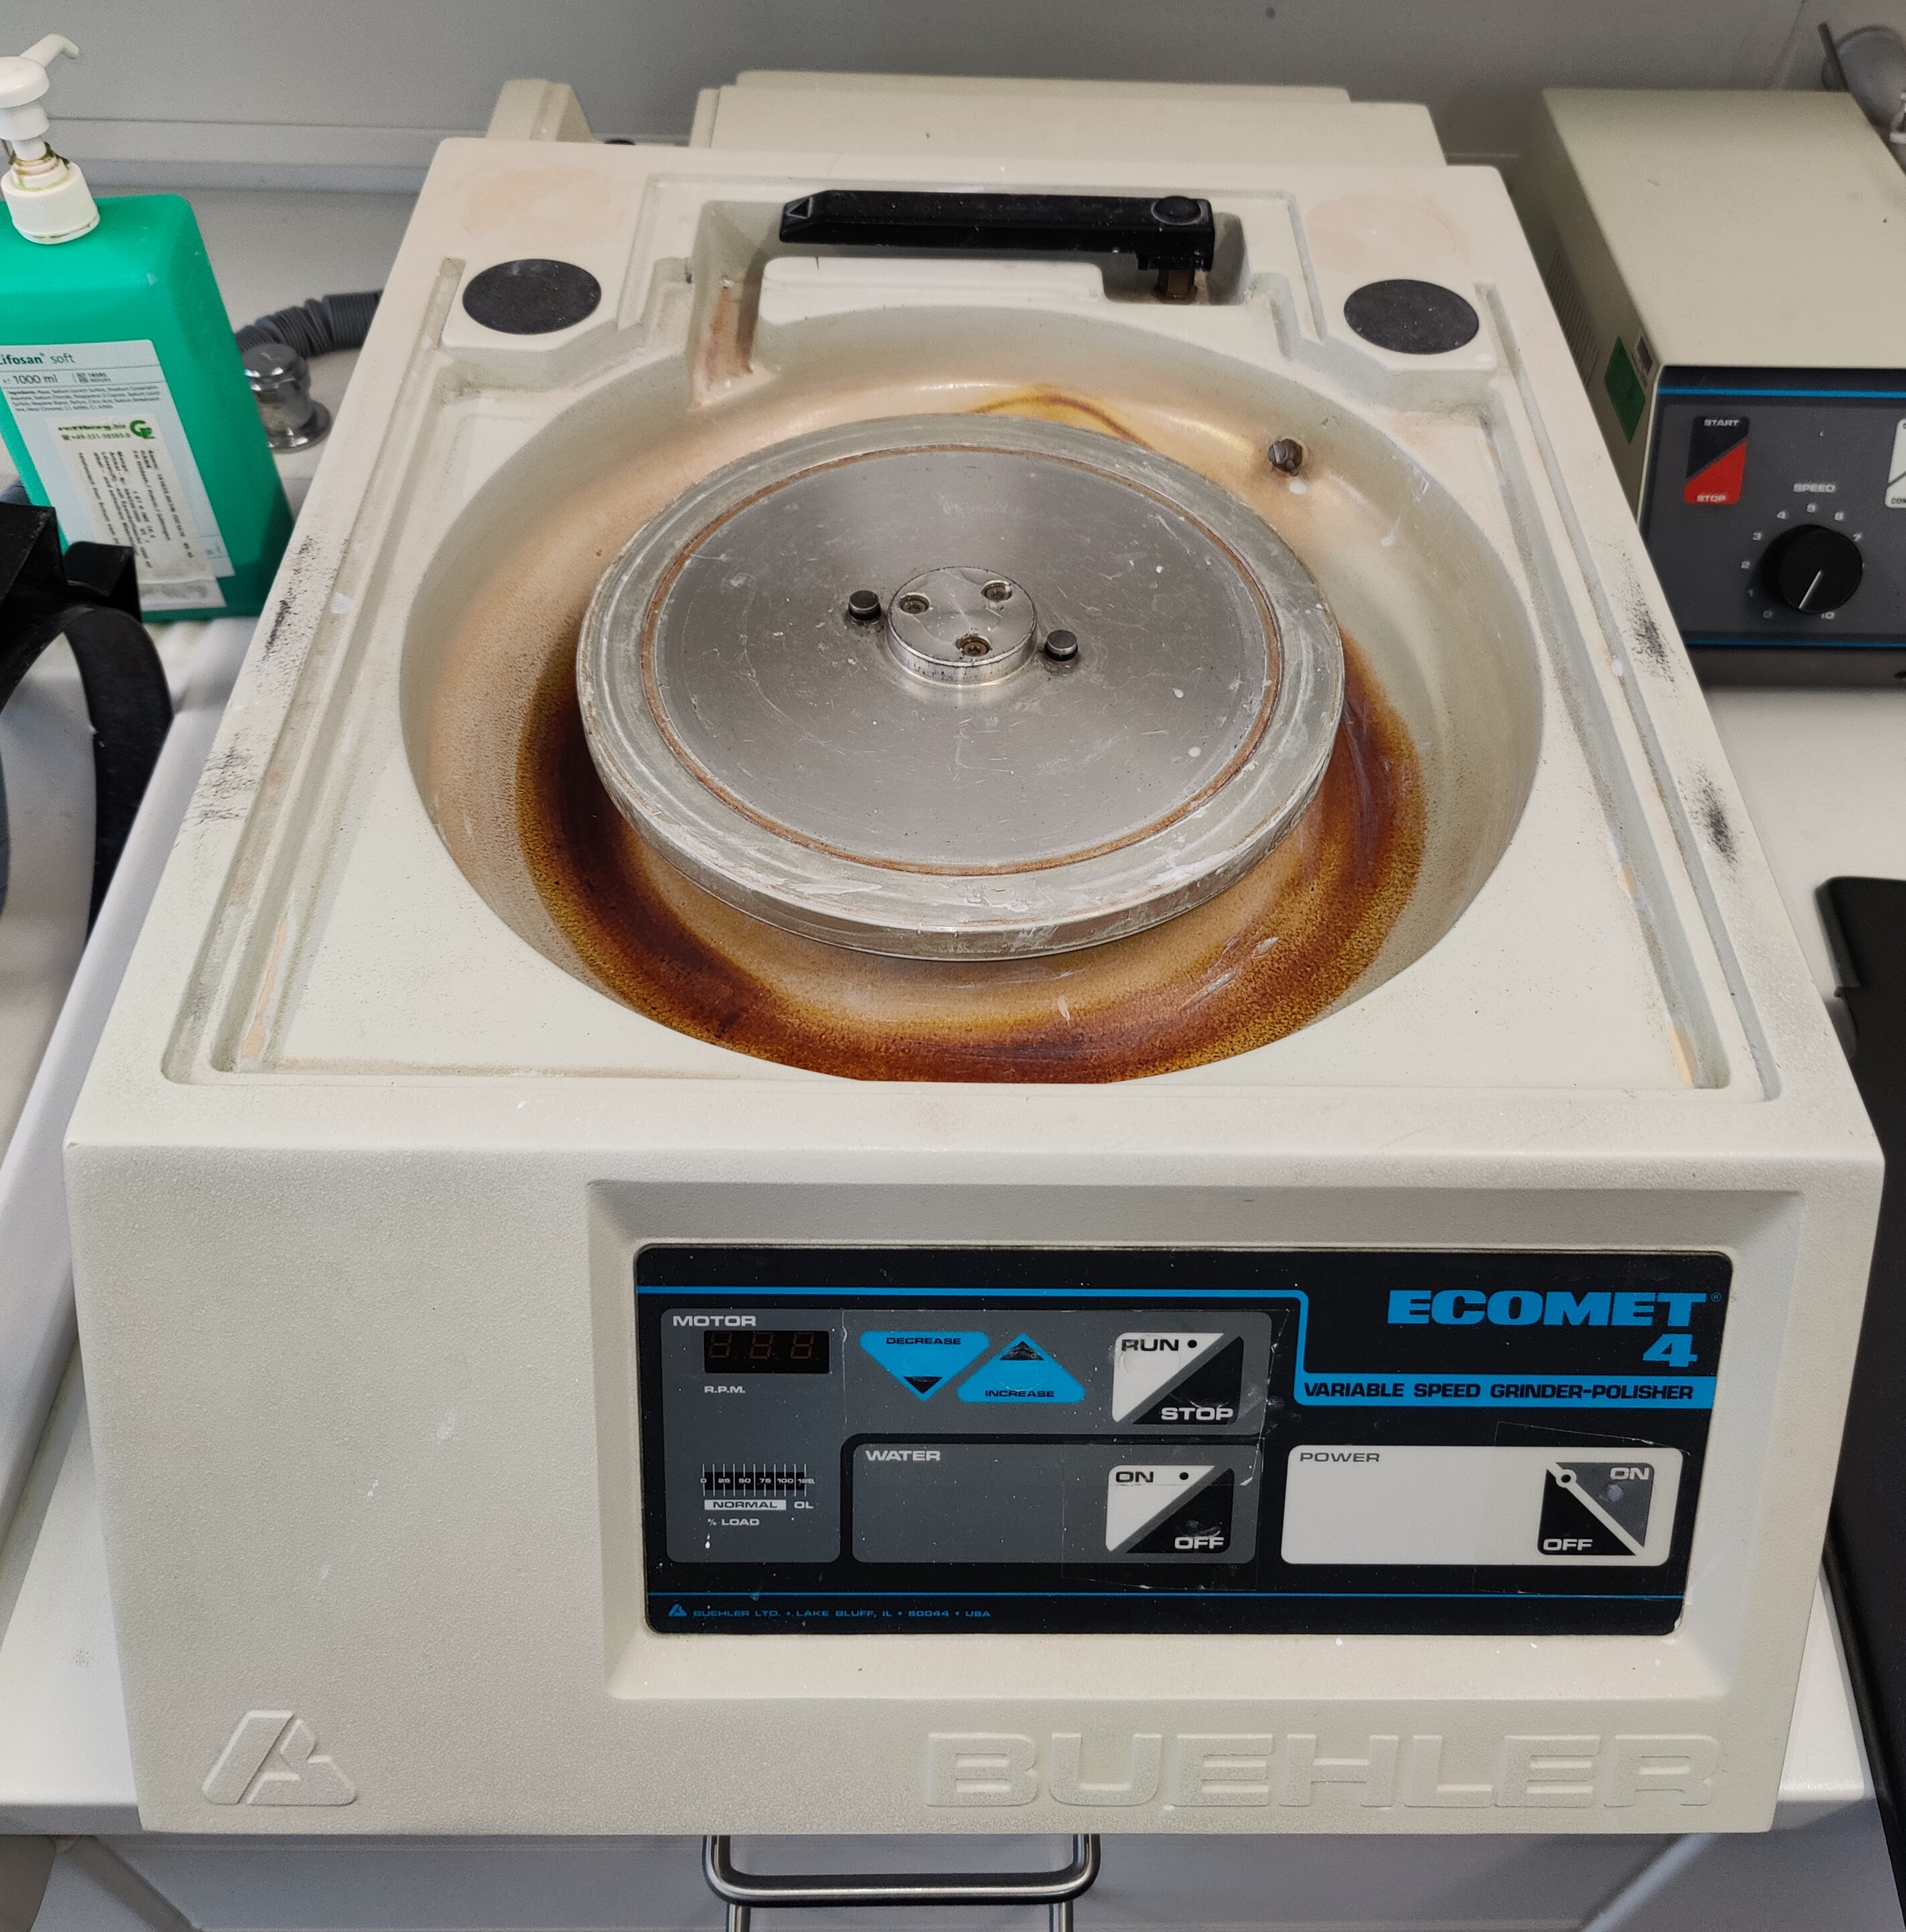
\includegraphics[width = 0.5\textwidth]{chapter_3/polish_setup_graphs/ecomet_4.jpg} 
    %\vspace*{-30pt}
    \caption{Photograph of the Ecomet 4.}
    \label{fig:ecomet_4}
\end{figure}
The apparatus is composed of a rotating platen on which either grinding paper or polishing cloth can be installed. The revolutions per minute (RPMs) of the platen could be easily modified to a specific value and, in addition, a constant source of tap water could be turned on. The machine is completely manual, meaning that the user needs to manually apply a down-pressing force upon the glass, while the platen is turning, to ensure correct contact between the platen itself and the sample.
\\
As anticipated before, long sessions of polishing needed to be carried out. To simplify the procedure and to reduce the influence of human error, an automatic way of holding and pressuring the sample was implemented.

\subsubsection{Sample Holder}
\label{subsubsec:sample_holder}
A simple block of machined aluminum, with carved out holes of the same size as the glass samples ($1\: cm$ of diameter and $2\: mm$ of thickness), was employed to hold the glass in place during both grinding and polishing. Using some small metal washers as spacers, it was possible to make the samples stick out from the holder, allowing only for their surface to make contact with the polishing pad. 

\begin{figure}[H]
    \centering
    \subfloat[Design of the holder. a) Holder, b) Washers, c) Glas samples, d) Polishing surface. \label{fig:holder_design}]{
        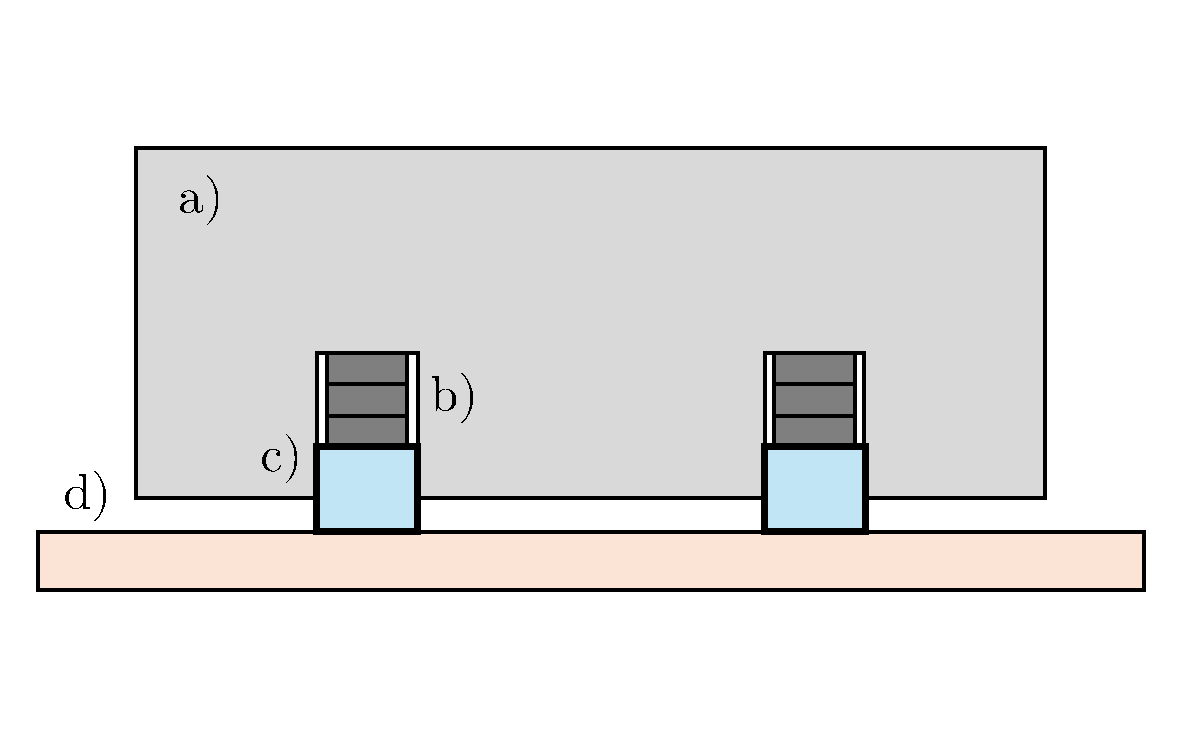
\includegraphics[scale=0.4]{chapter_3/polish_setup_graphs/holder_design.pdf}
    }
    \quad
    \subfloat[Photo of the holder. \label{fig:holder_photo}]{
        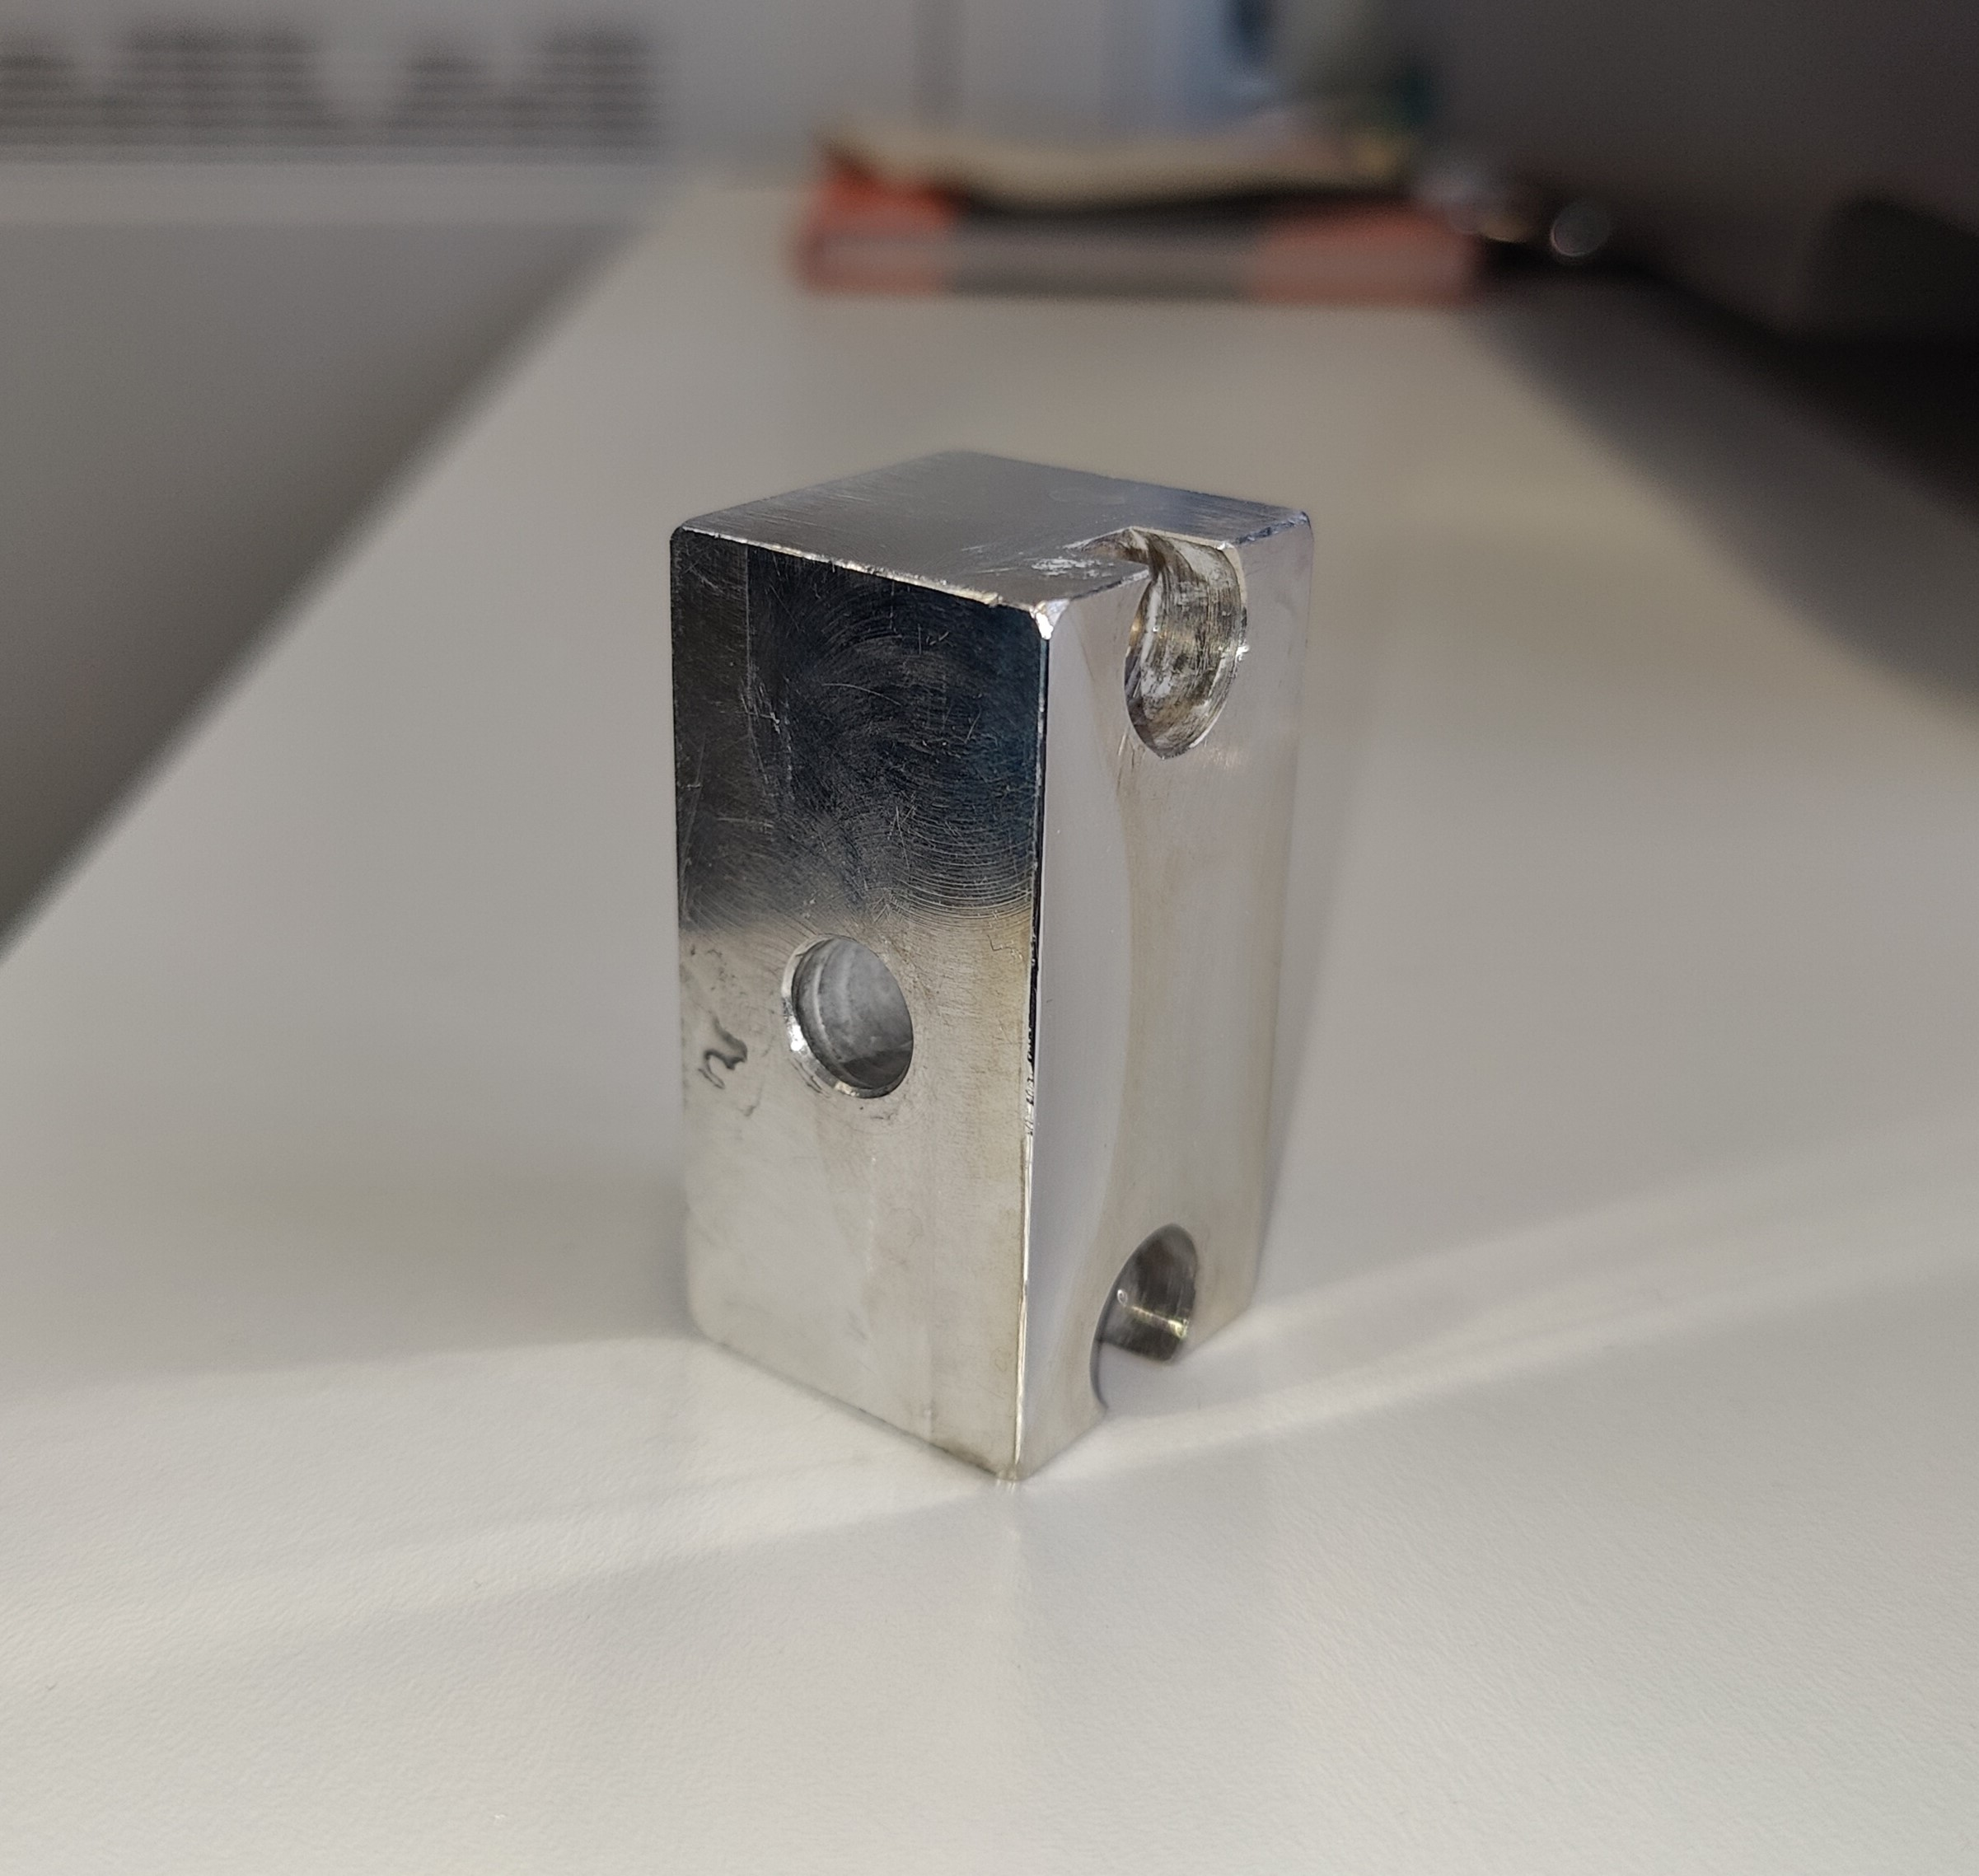
\includegraphics[scale=0.07]{chapter_3/polish_setup_graphs/aluminum_holder.jpg}
    }
    \caption{Aluminum holder for the glass samples. }
    \label{fig:holder}
\end{figure}
The aluminum block, while holding the glass samples, was held firm by another custom manufactured metal element, shown in Figure~\ref{fig:aluminum_structure}, that was anchored to the polishing machine frame. In this way, during both the grinding and the polishing phases, the holder could resist the friction forces caused by the 
platen rotation, maintaining fixed the sample position during the process.
\begin{figure}[H]
    \centering
    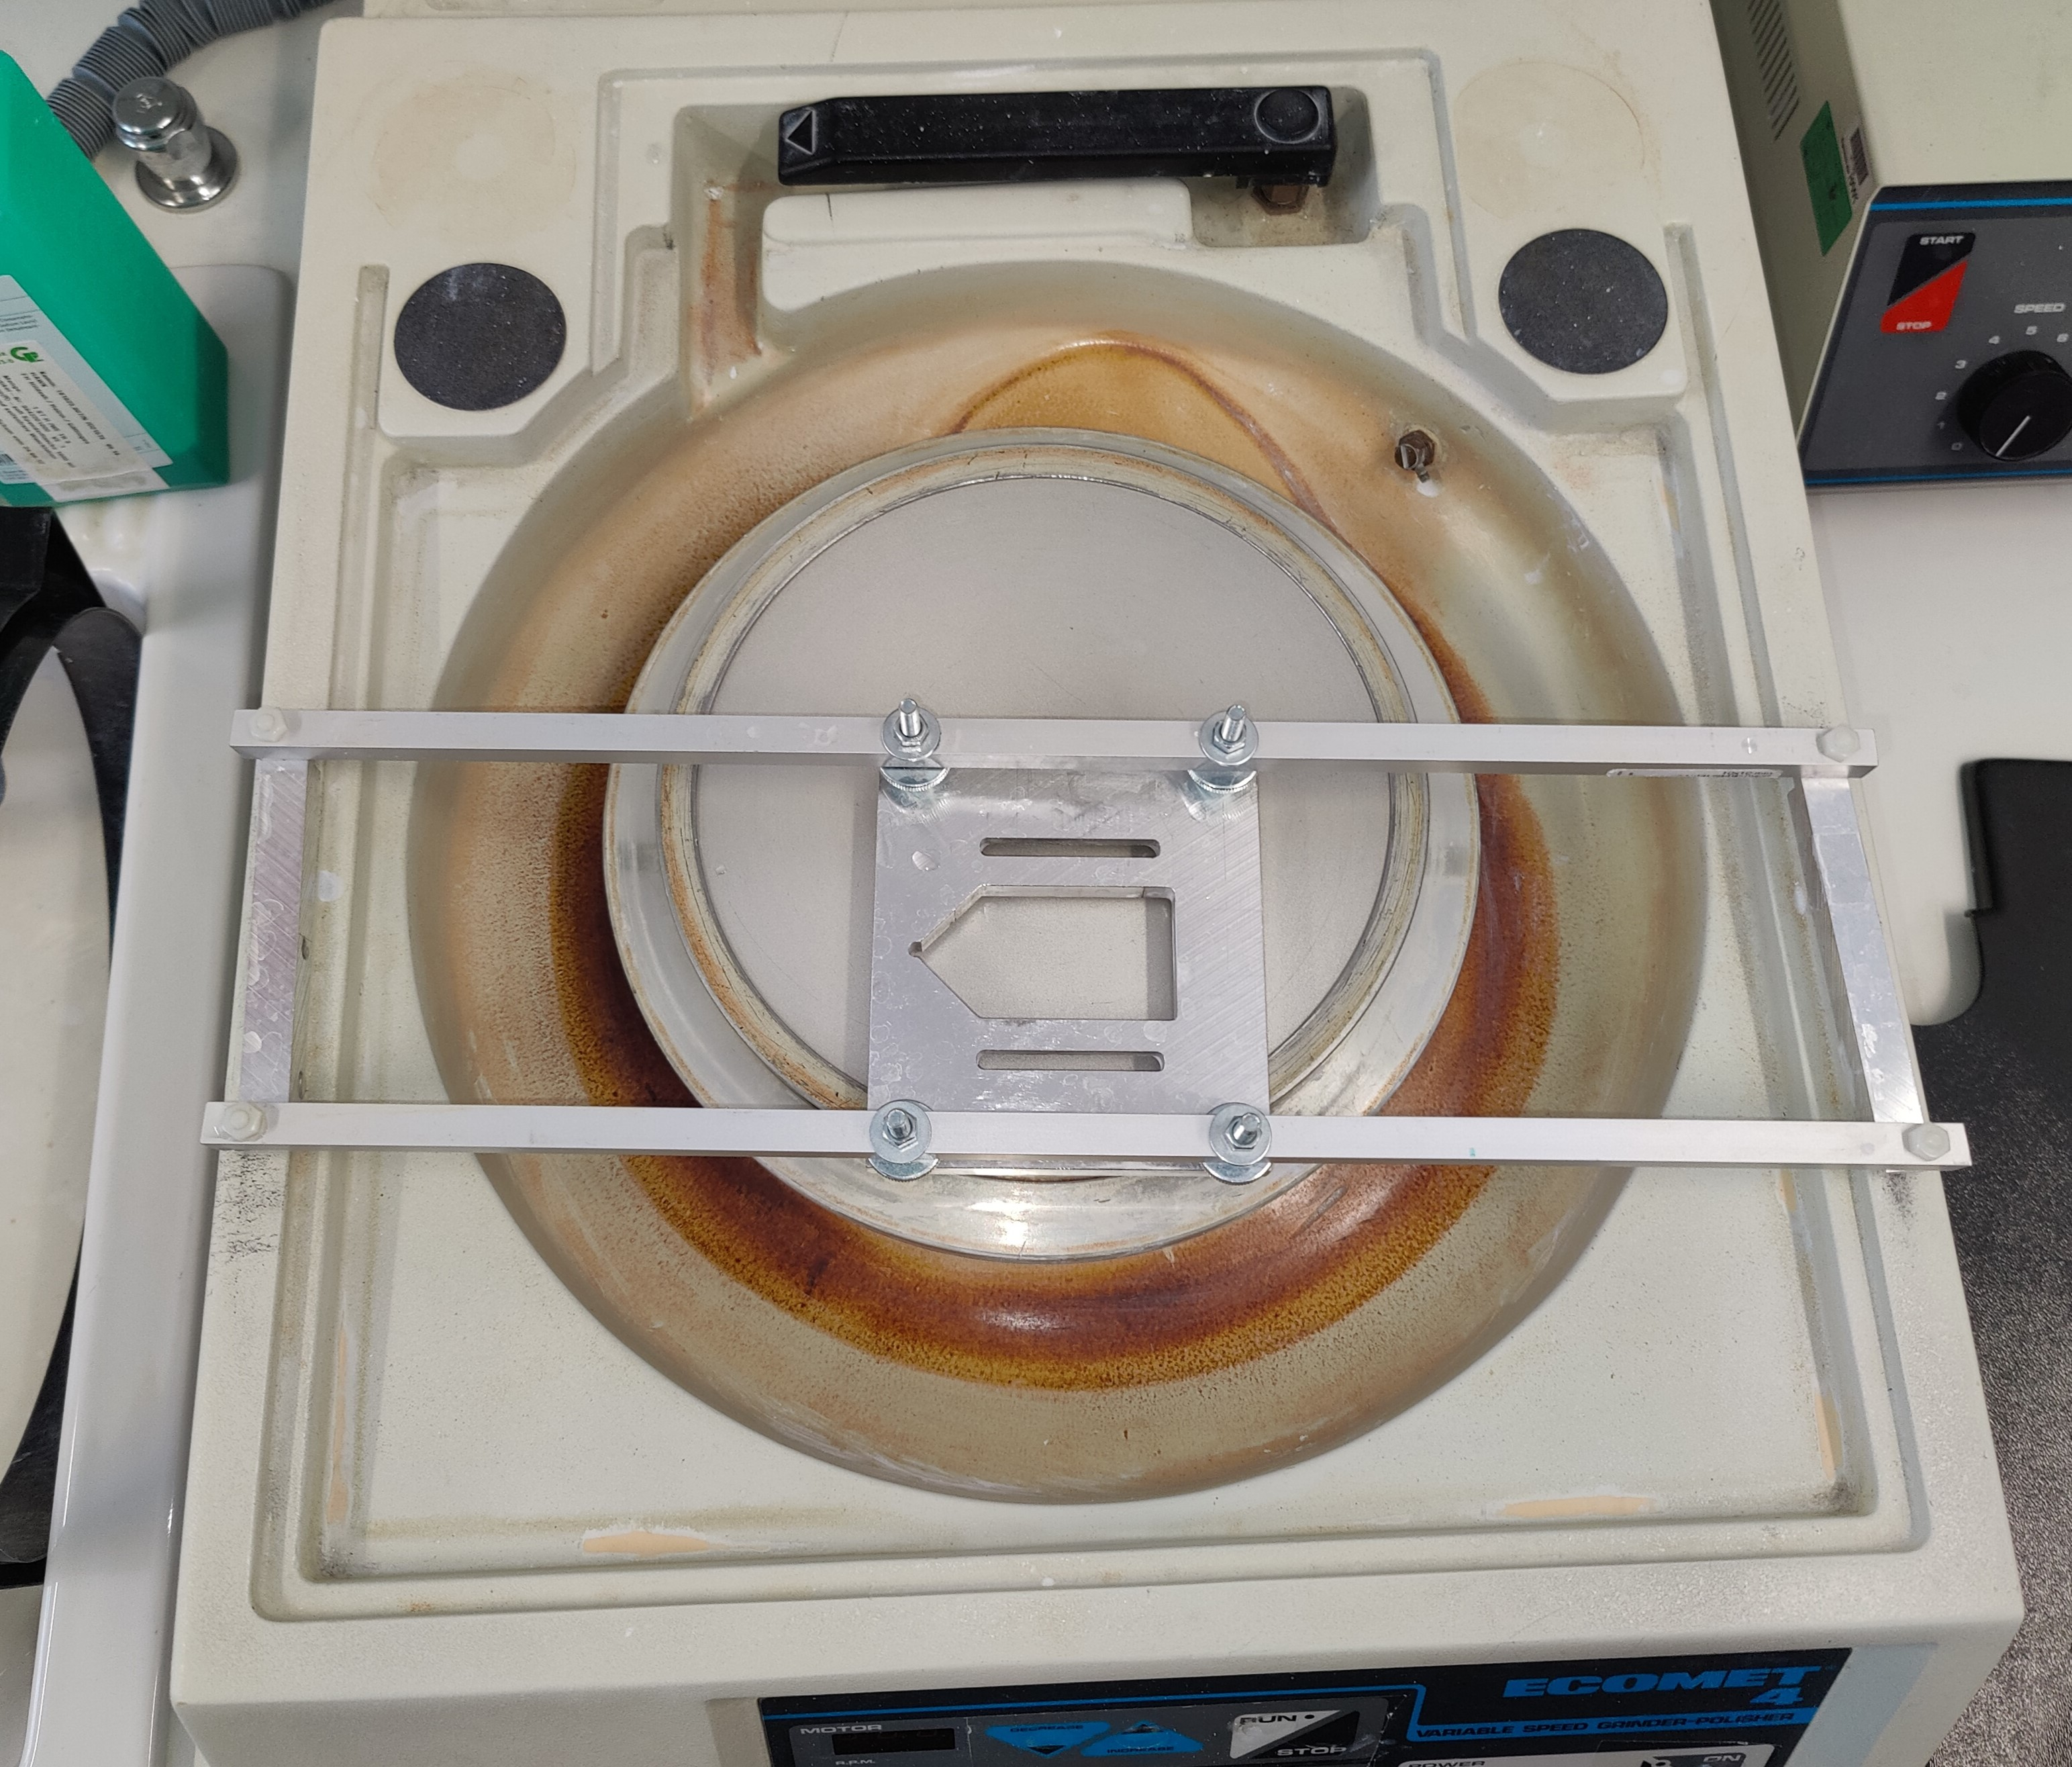
\includegraphics[width = 0.6\textwidth]{chapter_3/polish_setup_graphs/ecomet_holder.jpg} 
    %\vspace*{-30pt}
    \caption{Aluminum structure that constrained the movements of the holder.}
    \label{fig:aluminum_structure}
\end{figure}
In the end, the holder setup was completed utilizing a steel block with a weight of around $500\: g$, to create the necessary downforce with which to press the glass on the grinding or polishing surfaces. Considering that each of the glass sample had a diameter of $1\:cm$, the overall pressure felt by each piece is given by Equation~\ref{eq:pressure_on_glass}:
\begin{align}
    P=\frac{1}{2}\frac{gM}{\pi\left(d/2\right)^2}\approx30\ kPa \label{eq:pressure_on_glass}
\end{align}

\subsubsection{Grinding paper and polishing pad}
\label{subsubsec:grinding_paper_and_pad}
As for the grinding paper, a silicon carbide disk was employed, while for the polishing cloth, a magnetic backed 8 inches disk made of synthetic rayon was used.
\subsection{Parameters Chosen}
\label{subsec:parameters_chosen_polish}
To understand the relevant variables that could influence the introduction of contaminants in the glass, we had to choose a fixed number of possible parameters, from the ones listed at the start of Chapter~\ref{sec:pol_parameter}, that needed to vary between measurements.
\\
In a similar way done for the identification of the most valid LIBS parameter done in Chapter~\ref{subsec:parameters_chosen}, we did a set of tests to select the relevant variables that regarded the polishing process.

\subsubsection{Type of Glass}
Pure silica is not the only glass employed in optics, \ce{SiO2} is often doped with various compounds to tune the final refractive index of the material.
\\
The presence of other species could impact both physical and chemical properties of the glass, and, consequently, vary the contamination process.
\\
The two types of glass that were at our disposal were: pure silica, high purity samples provided by the manufacturer “QI Optiq”, and NZK-7, provided by the manufacturer “Schott”. 
\\
NZK-7 is a glass with a principal refractive index $n_d$, measured at $587.56 \: nm$, of 1.50847, and has an elemental composition displayed in Table~\ref{table:nzk7_concentration}:



\begin{table}[H]
    \centering
\begin{tabular}{|l|c|}
\hline
Chemical Name     & Concentration in Weight (\%) \\ \hline
Aluminum Oxide    & 1 - 10                         \\ \hline
Boron Oxide       & 10 - 20                        \\ \hline
Calcium Oxide     & \textless 1                  \\ \hline
Chlorine          & \textless 1                  \\ \hline
Sodium Oxide      & 1 - 10                       \\ \hline
Antimony Trioxide & \textless 1                  \\ \hline
Silica            & 60 - 70                        \\ \hline
Zinc Oxide        & 10 - 20                        \\ \hline
\end{tabular}
\caption{Chemical composistion of NZK-7 glass. }
    \label{table:nzk7_concentration}
\end{table}

In the composition it is important to notice the presence of compounds like aluminum oxide, calcium, zinc, and sodium. These elements are in fact part of the ones that we expect to introduce from the grinding and polishing process. Aluminum from the polishing suspension and the others from the tap water used in all the parts of the processing (the elemental composition of the tap water in Göttingen is shown in Table~\ref{table:water_composition}).
\\
The presence of these elements is confirmed by our measurements:
\begin{figure}[H]
    \centering
    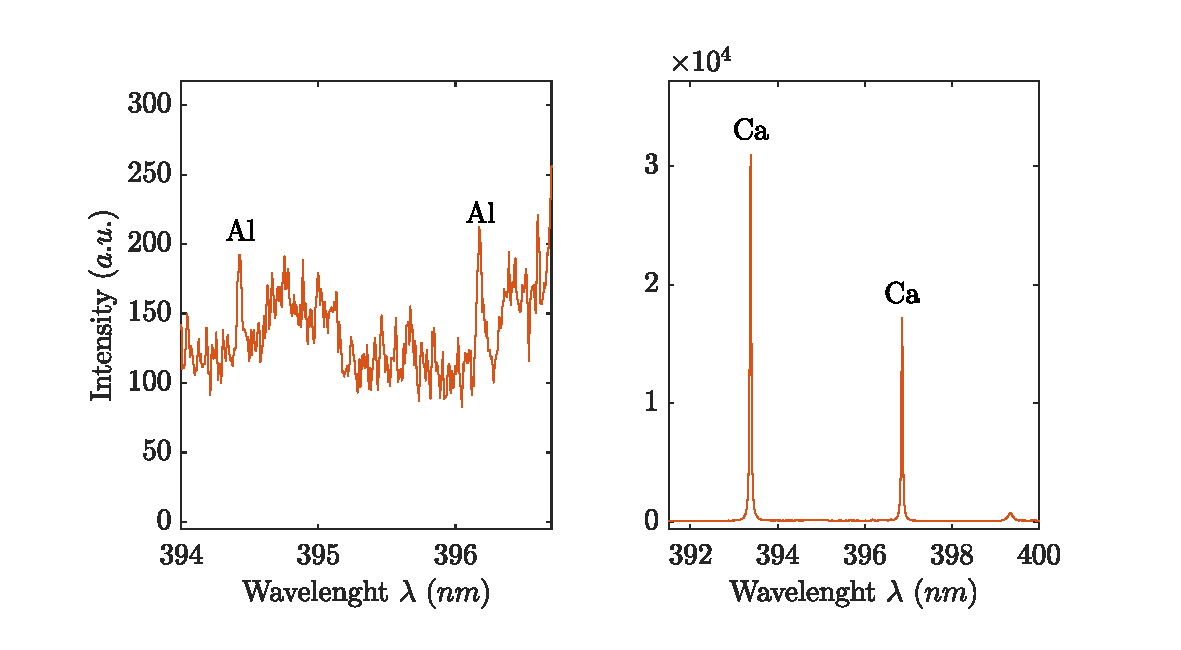
\includegraphics[width = \textwidth]{chapter_3/polish_setup_graphs/NZk7_contaminants_zoom.pdf} 
    \vspace*{-30pt}
    \caption{Focus on the aluminum and calcium peaks of NZK-7.}
    \label{fig:nzk7_aluminum_calcium}
\end{figure}
In Figure~\ref{fig:nzk7_aluminum_calcium} we can clearly see the presence of both aluminum and calcium peaks even in the “raw” sample. For this reason, we chose to not perform measurement on NZK-7 glass, it is much easier to track contaminants when the starting sample does not have the elements that we are searching for already in the spectrum.

\subsubsection{Type of Polishing Agent}
\label{subsubsec:polish_type_conc}
As already mentioned in Chapter~\ref{sec:pol_parameter}, the most common polishing suspensions used in optics manufacturing are \ce{Al2O3} and \ce{CeO2}. 
The specific products we employed were:

\begin{itemize}
    \item A cerium oxide-based mixture by the company GlassPolish, characterized by a particle size with an average of $2.5\: \mu m$ and a purity of more than 95\% as stated by the spec sheet.
    \item An aluminum oxide powder supplied by the company CharpauS, with a particle size between 2 and $6 \: \mu m$.
\end{itemize}

The limits of detection (LOD) of cerium and aluminum found in literature are, respectively, around $100 \: ppm$ and $1\: ppm$. [LOD taken from LIBS-info]
\\
By also looking at the theoretical emission spectra of cerium in Figure~\ref{fig:ce_plot_nist}, plotted from the information of the “relative intensity” on the NIST database, it is evident that there is no single peak that stands out and can therefore be easily identified. Emission lines cover almost continuously the whole spectrum from $350 \: nm$ to $500 \: nm$.
\begin{figure}[H]
    \centering
    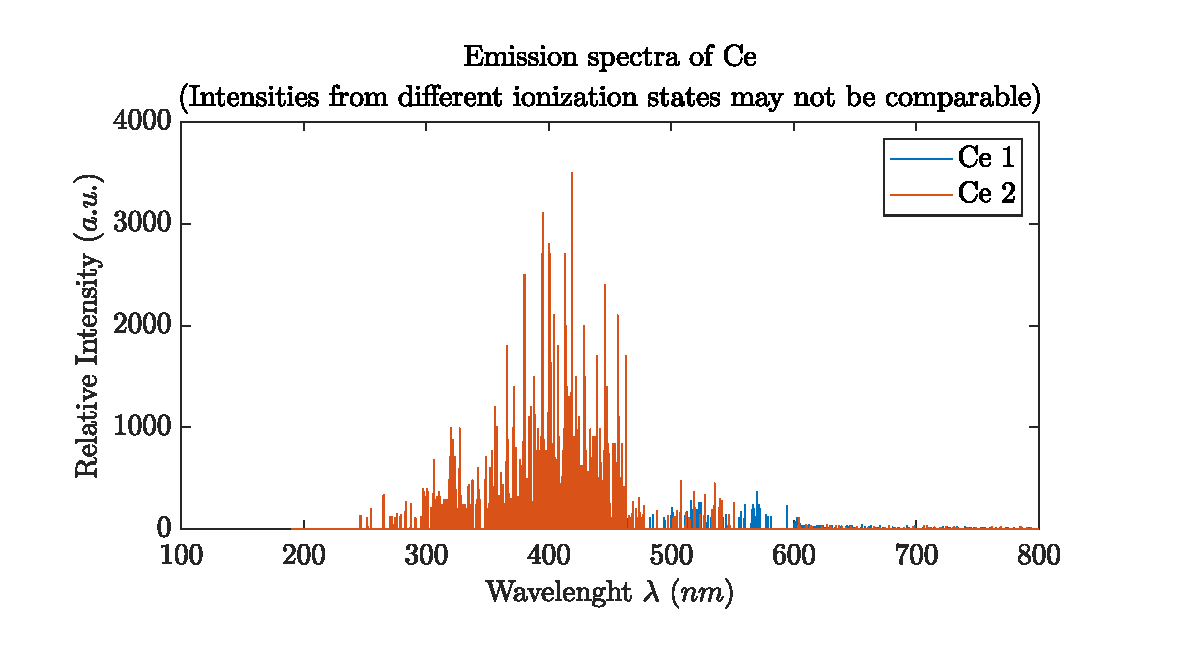
\includegraphics[width = \textwidth]{chapter_3/polish_setup_graphs/spectra_cerium.pdf} 
    \vspace*{-30pt}
    \caption{Spectra of cerium plotted from the information in the NIST database. }
    \label{fig:ce_plot_nist}
\end{figure}
This combined with the high LOD makes it particularly difficult to find this element in low concentrations using LIBS.
\\
In Figure~\ref{fig:ce_peaks_raw_polished} there is the comparison between the spectra of the same glass sample, raw and after one hour of polishing. In the highlighted spectral regions, there should be two intense cerium lines. It is clear that that even after 
\begin{figure}[H]
    \centering
    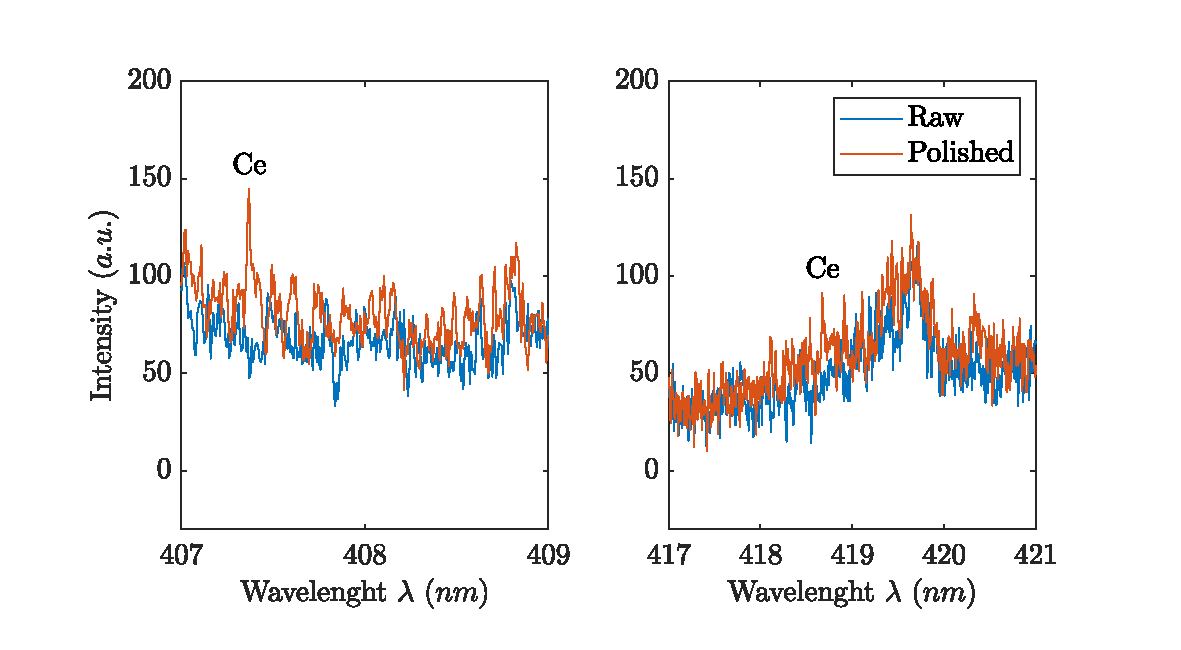
\includegraphics[width = \textwidth]{chapter_3/polish_setup_graphs/raw_polished_siO2_cerium.pdf} 
    \vspace*{-30pt}
    \caption{Cerium peaks compared in spectra before and after polishing. }
    \label{fig:ce_peaks_raw_polished}
\end{figure}
Under these conditions, it would be impossible to do any meaningful quantitative analysis. In the end we decided to focus our attention only on polishing with the alumina-based polishing agent.

\subsubsection{Polish Concentration}
\label{subsubsec:polish_concentration_setup}

As already mentioned in Chapter~\ref{sec:pol_parameter} the polish concentrations commonly used in optics manufacturing are between 5\% and 30\%. For our measurements we decided to take as sample concentrations 5\%, 15\% and 30\%. 

\subsubsection{Grinding and Polishing Times}
\label{subsubsec:grinding_pol_times}
Considering that diffusion is a time-dependent process we expect to have some dependencies on grinding and polishing time.
\\
To reduce the amount of variable we had to control, we decided to fix the grinding time to 3 minutes for every sample.
\\
Regarding polishing, expecting a dependence in the contaminants' concentration that was logarithmic/exponential with respect to time, we decided to take measurements not at fixed time intervals but instead to double the amount of time between each evaluation. From one minute to two hours of polishing.
\\
As a summary, the measurements were taken at: 
Raw, ground ($3\: min$), $1\: min$, $2\: min$, $4\: min$, $8\: min$, $15\: min$, $30\: min$, $1\: h$ and $2\: h$.

\subsection{Measurements of Polishing Components}
\label{subsec:measurements_pol_components}
In this section will be presented the results of LIBS analysis performed on all the components that were in direct contact with the samples and were therefore capable of introducing contaminants into the glass. In addition, a list of the elements dissolved in tap water is printed.

\subsubsection{Polishing Powders}
\label{subsubsec:meas_pol_powders}
LIBS analysis performed on a tablet of compressed aluminum oxide powder showed a very low presence of elements other than aluminum. Precisely calcium is present at a relative concentration lower than 1\% while only a few traces of copper and gallium were detected.

\subsubsection{Silicon Carbide Grinding Paper}
\label{subsubsec:grinding_paper_meas}
Some LIBS analyses were also performed on a sample of unused grinding paper. Sodium was found to be present at a very high relative concentration of about 10\%. A small portion of contaminants such as calcium and iron were found with concentrations lower than 0.5\%, while the presence of other traces elements, such as magnesium and lanthanum, was also detected with concentrations in the order of few ppm.

\subsubsection{Polishing Pad}
\label{subsubsec:polishing_pad_meas}
The polishing pad was also subjected to the same kind of analysis. Not surprisingly, the results of the measurement showed that the main component of the pad is carbon, as it is the main constituent of the rayon fiber. Silicon has also been found present with a relative concentration of about 5\% while calcium only in concentrations smaller than 1\%.


\subsubsection{Tap Water Chemical Composition}
\label{subsubsec:polishing_pad_meas}
The type of water mostly used in the optics manufacturing industry is tap water. In Germany, public water quality is periodically checked and an elemental composition analysis for the tap water in Göttingen is easily accessible from public databases. In Table~\ref{table:water_composition} are shown the main elements dissolved in the water we used during both the grinding and polishing processes:

\begin{table}[H]
    \centering 
    \begin{tabular}{|l|c|c|}
    \hline
                                   & Unit   & \multicolumn{1}{l|}{Value Range} \\ \hline
    Water Temperature              & °C     & 5,9-16,7                                  \\ \hline
    PH Value                       &        & 7,7-8,2                                   \\ \hline
    Total alkaline earths          & mol/m³ & 1,4                                       \\ \hline
    Calcium                        & mg/l   & 40,1-42,5                                 \\ \hline
    Magnesium                      & mg/l   & 7,33-9,03                                 \\ \hline
    Sodium                         & mg/l   & 7,4-10,9                                  \\ \hline
    Potassium                      & mg/l   & 0,9-1,3                                   \\ \hline
    Chloride                       & mg/l   & 10,8-14,7                                 \\ \hline
    Nitrate                        & mg/l   & 14,9-19,3                                 \\ \hline
    Sulfate                        & mg/l   & 25-35                                     \\ \hline
    Phosphorus Compounds           & mg/l   & \textless{}0,1                            \\ \hline
    Silicon Compounds              & mg/l   & 5,0-7,4                                   \\ \hline
    Organically Bound Carbon (TOC) & mg/l   & 0,7-1,0                                   \\ \hline
    Aluminum                       & mg/l   & 0,02-0,03                                 \\ \hline
    Oxygen                         & mg/l   & 9,2-13,0                                  \\ \hline
    \end{tabular}
    \caption{Chemical composition of tap water in Göttingen in 2023.}
        \label{table:water_composition}
    \end{table}

With the goal of partially mitigating the contamination process on the surface of the glass sample caused by water, some experiments were carried out employing only distilled water from the start to the end of the procedure.
\\
This was particularly challenging due to the need to ensure the contact of the glass only with instruments washed with distilled water, from the glassware, where the polishing slurry was prepared, to the tweezers used to handle the samples. The grinding paper and the polishing pad also had to be replaced constantly for the same reason.
\\
But due to the extremely high solubility of distilled water, the risk of accidentally dissolving species into the solution was always a concern.

\section{Other apparatuses}
\label{sec:other_apparatuses}
Other than LIBS, experiments were also carried out on FTIR, XPS and contact angle measuring systems. Since they were not the focus of our research, in this section will be presented only a brief description of the apparatuses we used.

\subsection{FTIR}
\label{subsec:ftir_setup}
For FTIR measurements we employed the “Frontier” apparatus manufactured by PerkinElmer.
\\
Considering that our main concern regarded finding contaminants at the surface of our samples, we used a setup to perform “Internal Reflectance Spectroscopy”, a technique we described in short in Chapter~\ref{sec:ftir}.
\\
During measurements, a lot of issues were caused by the lack of consistency between different evaluations of the same sample measured multiple times in a row, in the same exact conditions. A crucial requirement of this technique is achieving perfect contact between the glass and the high refractive index material in the machine, using a plastic spacer to ensure even pressure on the small glass sample was not enough.
\\
Even though the presence and position of the absorption peaks remained constant, the absolute value of the absorption could vary a lot.
\\
In Figure~\ref{fig:ftir_issues} are shown different FTIR measurements of the same sample, the runs were done by simply removing and replacing the material from the apparatus.

\begin{figure}[H]
    \centering
    \includegraphics[width = \textwidth]{chapter_3/other_apapratuses_graphs/FTIR_issues.pdf} 
    \vspace*{-30pt}
    \caption{Various FTIR measurements made to the same sample with internal reflectance spectroscopy.}
    \label{fig:ftir_issues}
\end{figure}

In the plot we can see that even the transmission at the wavenumber range between 4000 and $1500\: cm^{-1}$, that for glass should always be around 100\%, spans from more than 100\% to 60\%.

\subsection{Contact Angle Measurement}
\label{subsec:contact_angle_setup}
The contact angle measurement apparatus was provided by the Kruss company, specifically, the DSA100E automated system.
\\
Experiments were carried out using water (\ce{H2O}) and diiodomethane (\ce{ CH2I2}) as, respectively, polar and apolar probe liquids.
\\
This technique is very sensible to surface characteristics and particular attention must be paid to avoid unwanted depositions of external substances. In our case, we discovered that cleaning between measurements with isopropanol could heavily influence the evaluation of the contact angle.  
\\ 
By looking at the surface of the glass with a microscope, as shown in Figure~\ref{fig:surface_droplets}, we could clearly see the presence of microdroplets of isopropyl alcohol, even hours after the cleaning. 

\begin{figure}[H]
    \centering
    \includegraphics[width = 0.8\textwidth]{chapter_3/other_apapratuses_graphs/surface_droplets.png} 
    %\vspace*{-30pt}
    \caption{Surface of a glass sample cleaned with isopropanol.}
    \label{fig:surface_droplets}
\end{figure}

To ensure that the droplets were evaporated completely, the samples were put in an oven for 40 minutes at a temperature of $60\: ^{\circ} C$ after each cleaning.

\subsection{XPS}
\label{subsec:xps_setup}
The XPS apparatus that measured our samples is a PHI VersaProbe II from Ulvac-phi. The model uses a monochromatic \ce{Al-K$\alpha$} source with a photon energy of $1486.6 \: eV$. The applied X-ray source has a power of 100 W.
\\
As explained in Chapter~\ref{sec:xps}, the XPS analysis is sensitive to just a few monolayers of the surface of the sample. To carry out depth resolved examinations, a small portion of the sample is removed from the surface with ion etching and consecutive measurements are conducted until the desired depth is reached.
\\
In our case, z-resolution was not one of the focuses of our research, so the XPS measurements were done only one time per sample, after surface cleaning had been performed with ion etching.



\chapter{Experimental Results}
\label{ch:experimental_results}

\section{FTIR}
\label{sec:ftir_results}
Here are presented the FTIR spectra of a raw, ground and polished sample. 

\begin{figure}[H]
    \centering
    \includegraphics[width = \textwidth]{chapter_5/others/ftir_plot.pdf} 
    \vspace*{-30pt}
    \caption{FTIR spectra.}
    \label{fig:ftir_plot}
 \end{figure}

As already said in Chapter~\ref{fig:ftir_issues} the differences in amplitude are not relevant but only the position and presence of transmission dips. 
\\
From Figure~\ref{fig:table_inorganic} we can identify that the two major peaks present in the spectra, at $1000 \:cm^{-1} $and $780 \:cm^{-1}$, respectively corresponds to \ce{SiO2} and \ce{SiO3} compounds, that are the main constituent in silica glass.
\\
\begin{figure}[H]
    \centering
    \includegraphics[width = \textwidth]{chapter_5/others/ftir_plot_zoom.pdf} 
    \vspace*{-30pt}
    \caption{Focus on the notable spectral range of the FTIR measurements.}
    \label{fig:ftir_zoom_plot}
 \end{figure}

The small dip at $1173 \:cm^{-1}$, that can be seen more clearly in Figure~\ref{fig:ftir_zoom_plot}, is associated to \ce{C-O} stretching \cite{chunliwang991FTIRFunctionalGroup2021} and could be caused by carbonaceous compounds that are present on the surface as residues from the cutting process \cite{kohlerQuantificationCarbonicContamination2021}. The absorption, in fact, disappears for the ground and polished sample, showing that the contamination came from manufacturing, and was then removed with our procedures.
\\
This is in line from what has already been found here [paper robert kohler].

\section{Contact Angle Measurement}
Contact angle measurements were also performed on the raw and on a polished sample. The results are presented in the Figure~\ref{fig:contact_angle_raw_polished}.
\begin{figure}[H]
    \centering
    \includegraphics[width = \textwidth]{chapter_5/others/contact_angle.pdf} 
    \vspace*{-30pt}
    \caption{Contact angle measurements for a raw and a polished sample. }
    \label{fig:contact_angle_raw_polished}
 \end{figure}
Considering the differences in the average value of the measured angle between the polar and the non-polar probe liquids, there could be a change in the contributions to the surface energy of the glass. Specifically, it does not seem that the polar fraction of surface energy has been affected by the polishing. However, in the case of diiodomethane, both the mean and the standard deviation notably changed for the two sample. The shift in the mean can be explained by the presence of carbonaceous compounds on the surface of the glass as a side effect of the manufacturing process, supporting what has been found with FTIR measurements in Chapter~\ref{sec:ftir_results}.
\\
Contact angle values are also influenced by the roughness of the surface, this could explain the decrease in standard deviation of the polished sample.

\section{XPS}
\label{sec:xps_results}
XPS analyses was done to confirm the presence of the contaminants with a more precise technique, check for species that are not easily detectable by LIBS and to see if chemical shift is present in the spectra of aluminum, silicon and carbon. This would imply the formation of new chemical species during the polishing phase.
\\
The measurements were performed on raw and polished samples. The results are presented in the following figures.
\\


\begin{figure}[H]
   \centering
   \includegraphics[width = \textwidth]{chapter_5/others/XPS/XPS_Ca_conc.pdf} 
   \vspace*{-30pt}
   \caption{Calcium concentration measured by XPS. }
   \label{fig:ca_xps}
\end{figure}


\begin{figure}[H]
   \centering
   \includegraphics[width = \textwidth]{chapter_5/others/XPS/XPS_Al_conc.pdf} 
   \vspace*{-30pt}
   \caption{Aluminum concentration measured by XPS. }
   \label{fig:al_xps}
\end{figure}

\begin{figure}[H]
   \centering
   \includegraphics[width = \textwidth]{chapter_5/others/XPS/XPS_Na_conc.pdf} 
   \vspace*{-30pt}
   \caption{Sodium concentration measured by XPS. }
   \label{fig:na_xps}
\end{figure}


Calcium, aluminum and sodium impurities were found in the XPS measurements. In the case of aluminum and sodium, it appears that their concentration is increasing as the polish concentration increases. However, calcium present the opposite behavior.

\begin{figure}[H]
   \centering
   \includegraphics[width = \textwidth]{chapter_5/others/XPS/XPS_K_conc.pdf} 
   \vspace*{-30pt}
   \caption{Potassium concentration measured by XPS. }
   \label{fig:k_xps}
\end{figure}
\begin{figure}[H]
   \centering
   \includegraphics[width = \textwidth]{chapter_5/others/XPS/XPS_Zn_conc.pdf} 
   \vspace*{-30pt}
   \caption{Zinc concentration measured by XPS. }
   \label{fig:zn_xps}
\end{figure}

Traces of zinc and potassium have also been found, these species were never detected during our LIBS measurements. The potassium impurities were expected due to its presence in the tap water, as shown in Table~\ref{table:water_composition}.
\\
The dependence of Zinc relatively to the polish concentration has a decreasing behavior, similar to calcium.
\\
None of the contaminants were absent from the measurement of the samples polished with the solution made with distilled water.

\begin{figure}[H]
   \centering
   \includegraphics[width = \textwidth]{chapter_5/others/XPS/XPS_C_conc.pdf} 
   \vspace*{-30pt}
   \caption{Carbon concentration measured by XPS. }
   \label{fig:c_xps}
\end{figure}
The most intense carbon peak in LIBS is at $165 \: nm$, outside the range of our detector. For this reason the use of XPS to measure the concentration of this element was particularly important.
\\
Figure~\ref{fig:c_xps} shows a concentration of carbon both in the raw and the polished samples. The presence of carbonaceous compounds on the surfaces of the raw sample was already partially confirmed by the FTIR analysis in the form of a \ce{C-O} absorption peak (Chapter~\ref{sec:ftir_results}), while no traces were found in the ground and polished samples with the same technique. This could suggest that the nature of the carbon contaminants found on the raw and processed glass surfaces are different.
\\
Regarding chemical shift, here are presented the comparison between peaks of different samples:

\begin{figure}[H]
   \centering
   \includegraphics[width = \textwidth]{chapter_5/others/XPS/xps_chem_shift_si.pdf} 
   \vspace*{-30pt}
   \caption{Comparison of the \ce{Si}2p level measured with XPS. (Left) Raw sample. (Right) Polished sample.}
   \label{fig:xps_shift_si}
\end{figure}

\begin{figure}[H]
   \centering
   \includegraphics[width = \textwidth]{chapter_5/others/XPS/xps_chem_shift_al.pdf} 
   \vspace*{-30pt}
   \caption{Comparison of the \ce{Al}2p level measured with XPS. (Left) Polished with distilled water. (Right) Polished with tap water.}
   \label{fig:xps_shift_al}
\end{figure}

For what regards these elements, no new peak caused by chemical shift has been found.


\begin{figure}[H]
   \centering
   \includegraphics[width = \textwidth]{chapter_5/others/XPS/xps_chem_shift_c_corrected.pdf} 
   \vspace*{-30pt}
   \caption{Comparison of the \ce{C}1s level measured with XPS. (Left) Raw sample. (Right) Polished sample.}
   \label{fig:xps_shift_c}
\end{figure}

In Figure~\ref{fig:xps_shift_c} are present peaks that could be associated with the effect of chemical shift, however, a more probable explanation is that they are the 2p peaks of potassium. This is because the chemical shift that would correspond to those energies is associated with \ce{C-F} bonds, nonetheless, no traces of fluorine have been found from any analysis we performed.

\section{LIBS}
\label{sec:LIBS_measurements}

In this section are presented the experimental results of the LIBS measurements, as well as the fitting to the theoretical concentrations.
\subsection{Data Fitting Method}
\label{subsec:data_fitting}
As already explained in detail in Chapter~\ref{sec:theoretical_prediction}, if normal diffusion is the primary driving mechanism for the presence of contaminants in the glass, the expected concentration of contaminants should follow Equation~\ref{eq:c_bar_equation}.
\\
In the expression there are three different parameters that can influence the behavior of the function: $d_a$, $C_0$ and $D$. They are, respectively, the ablation depth of the LIBS measurement, the saturation concentration and the diffusion constant.
\\
The ablation depth should be the same for every measurement we performed, as it only depends on the laser parameters and on the target material, both of which were constant for all the experiments.
\\
To estimate this parameter we have performed some depth analyses with a 3D microscope on a pure silica sample that was ablated five different times with the same laser energy of $15 \: mJ$ but with an increasing number of pulses, from 5 to 25.

\begin{figure}[H]
    \centering
    \includegraphics[width = 0.8\textwidth]{chapter_5/LIBS/data_fit/3dmicroscope_profile.png} 
    \caption{Width and depth measurements of LIBS craters performed with a 3D microscope. The peaks are ordered from left to right accordingly to the number of pulses.}
    \label{fig:3d_microscope_craters}
 \end{figure}

 Unfortunately, due to the translucency of silica glass, optical measuring methods cannot be fully trusted, especially when performing depth profiling. The information presented in Figure~\ref{fig:3d_microscope_craters} is only useful to give an idea of the order or magnitude of the value.
 \\
For the first two peaks, the ones corresponding to 5 and 10 pulses, the depth measured by the microscope is around $5 \: \mu m$. In the case of our experiments the energy was the same but only one pulse was performed, with consequently less ablation. As an estimation of the crater depth, we considered the value cited before but one order of magnitude lower, $d_a = 0.5 \: \mu m$.
\\
The two other parameters, $C_0$ and $D$, strictly depend on the specific characteristics of the diffusion.
\\
The order of magnitude for $D$ in glasses can be found in literature; in Kawagishi et al. (1998)\cite{rathoreProceedingsSymposiumInterconnect1998} there is an estimation of the diffusion coefficient of gaseous metallic aluminum into the amorphous silica layer that forms on top of silicon wafers. The value is given by the following equation:
\begin{align}
    D/m^2s^{-1} = 1.83 \cdot 10^{-13}\exp \left(\frac{-1.12 \cdot 10^5}{RT}\right) \label{eq:diffiusion_coef_aluminum}
\end{align}
Where $R$ is the ideal gas constant and $T$ is the absolute temperature of the chamber. This expression is valid for values of the temperature between 973 and $1173 \:K$. By taking the middle value of that range, the corresponding $D$ is equal to $2.02 \cdot 10^{-18} \:m^2s^{-1}$.
\\
Regarding $C_0$, for the fitting procedure to make sense, the value of the parameter should be of the order of the experimental values; ideally, if the measurements follow a curve similar to the one in Figure~\ref{fig:c_bar_mixed}, the value of $C_0$ should be the one corresponding to the concentrations of the values taken at later polishing times.
\\
For the actual fitting, we employed a simple algorithm. We defined two arrays with the possible values of $D$ and $C_0$: for $D$ we constructed a logarithmic space between $10^{-20}$ and $10^{-7}$, while for $C_0$ we built a linear space between the minimum and two times the maximum the measured concentration of the element we were trying to fit.
\\
We then constructed another array with all the possible combinations between the two parameters, and, finally, we identified the couple that resulted in the least round mean square of the difference between the theoretical function and the data.
\\
The whole procedure should be enough to perform qualitative comparisons between different species.





\subsection{Concentration of the Polishing Solution}
\label{subsec:conc_results}
In the next section we will display all the collected data. Initially, for each polish concentration, a qualitative comparison of the notable wavelength ranges between the spectra of the raw, ground and polished (2 hrs) sample is shown. Secondly, the plots with the measured contaminants concentrations are presented. The diffusion parameters fitted with the method proposed in the previous section are also shown. Lastly, we will exhibit the differences between the measured contaminants relatively to the polish suspension concentration.
\\
The solutions with different concentrations and water types were also distinguished by a different level of pH, in Table~\ref{table:solution_ph} are shown the corresponding value. The values were all measured using litmus paper.

\begin{table}[H]
   \centering
   \begin{tabular}{lclll}
   \hline
   \multicolumn{1}{|c|}{Water Type} & \multicolumn{1}{c|}{Pure} & \multicolumn{1}{c|}{5pc}   & \multicolumn{1}{c|}{15pc}  & \multicolumn{1}{c|}{30pc} \\ \hline
   \multicolumn{1}{|c|}{Tap}        & \multicolumn{1}{c|}{6,5}  & \multicolumn{1}{c|}{6,5-7} & \multicolumn{1}{c|}{8-8,5} & \multicolumn{1}{c|}{9}    \\ \hline
   \multicolumn{1}{|c|}{Distilled}  & \multicolumn{1}{c|}{6}    & \multicolumn{1}{c|}{-}     & \multicolumn{1}{c|}{9}     & \multicolumn{1}{c|}{-}    \\ \hline
   \end{tabular}
   \caption{pH level of the polishing solutions relative to the concentration and type of water.}
        \label{table:solution_ph}
   \end{table}
\subsubsection{Polish Concentration: 5pc}
\label{subsubsec:5pc}

\begin{figure}[H]
    \centering
    \includegraphics[width = \textwidth]{chapter_5/LIBS/spectra_comparison/tap_5pc_first.pdf} 
    %\caption{Width and depth measurements of LIBS craters performed with a 3D microscope. The peaks are ordered from left to right accordingly to the number of pulses.}
    %\label{fig:3d_microscope_craters}
 \end{figure}

\vspace*{-71pt}
\begin{figure}[H]
    \centering
    \includegraphics[width = \textwidth]{chapter_5/LIBS/spectra_comparison/tap_5pc_second.pdf} 
    %\caption{Width and depth measurements of LIBS craters performed with a 3D microscope. The peaks are ordered from left to right accordingly to the number of pulses.}
    %\label{fig:3d_microscope_craters}
 \end{figure}


\begin{figure}[H]
    \centering
    \includegraphics[width = \textwidth]{chapter_5/LIBS/spectra_comparison/tap_5pc_third.pdf} 
    %\caption{Width and depth measurements of LIBS craters performed with a 3D microscope. The peaks are ordered from left to right accordingly to the number of pulses.}
    %\label{fig:3d_microscope_craters}
 \end{figure}

 As it can be seen from the plots, the polished sample can be easily distinguished from the other two spectra; in particular, the aluminum peaks are present only in the polished sampled, while the other elements are found also in the raw and ground spectra. Due to the lower sensitivity of the detector in the visible range, the sodium peak cannot be easily distinguished from the noise floor. Its presence is expected since, as shown in Table~\ref{table:water_composition}, a non-negligible quantity is dissolved in the water. Moreover, sodium has a low LOD \cite{mansooriQuantitativeAnalysisCement2011} and should be easily detectable with LIBS.
\\
For the next series of graphs, only the time evolution of the polishing phase is shown.
\begin{figure}[H]
    \centering
    \includegraphics[width = \textwidth]{chapter_5/LIBS/data_fit/fit_tap_5pc_Mg.pdf} 
    %\caption{Width and depth measurements of LIBS craters performed with a 3D microscope. The peaks are ordered from left to right accordingly to the number of pulses.}
    %\label{fig:3d_microscope_craters}
 \end{figure}
\vspace*{-48pt}
 \begin{figure}[H]
    \centering
    \includegraphics[width = \textwidth]{chapter_5/LIBS/data_fit/fit_tap_5pc_Ca.pdf} 
    %\caption{Width and depth measurements of LIBS craters performed with a 3D microscope. The peaks are ordered from left to right accordingly to the number of pulses.}
    %\label{fig:3d_microscope_craters}
 \end{figure}
 \begin{figure}[H]
    \centering
    \includegraphics[width = \textwidth]{chapter_5/LIBS/data_fit/fit_tap_5pc_Al.pdf} 
    %\caption{Width and depth measurements of LIBS craters performed with a 3D microscope. The peaks are ordered from left to right accordingly to the number of pulses.}
    %\label{fig:3d_microscope_craters}
 \end{figure}

    \vspace*{-20pt}
 \begin{figure}[H]
    \centering
    \includegraphics[width = \textwidth]{chapter_5/LIBS/Tap_elem_comparisons/Tap_elements_5_pc.pdf} 
    \vspace*{-30pt}
    \caption{Comparison of the concentration values of the major contaminants as a function of the polishing time, for the glass polished with a 5pc suspension.}
    \label{fig:tap_elem_5pc}
 \end{figure}
 In Figure~\ref{fig:tap_elem_5pc} it is clear that all the elements share a similar decreasing behavior.





\pagebreak



\subsubsection{Polish Concentration: 15pc}
\label{subsubsec:15pc}
\vspace*{-25pt}
\begin{figure}[H]
    \centering
    \includegraphics[width = \textwidth]{chapter_5/LIBS/spectra_comparison/tap_15pc_first.pdf} 
    %\caption{Width and depth measurements of LIBS craters performed with a 3D microscope. The peaks are ordered from left to right accordingly to the number of pulses.}
    %\label{fig:3d_microscope_craters}
 \end{figure}

\vspace*{-68pt}
\begin{figure}[H]
    \centering
    \includegraphics[width = \textwidth]{chapter_5/LIBS/spectra_comparison/tap_15pc_second.pdf} 
    %\caption{Width and depth measurements of LIBS craters performed with a 3D microscope. The peaks are ordered from left to right accordingly to the number of pulses.}
    %\label{fig:3d_microscope_craters}
 \end{figure}

\vspace*{-68pt}
\begin{figure}[H]
    \centering
    \includegraphics[width = \textwidth]{chapter_5/LIBS/spectra_comparison/tap_15pc_third.pdf} 
    %\caption{Width and depth measurements of LIBS craters performed with a 3D microscope. The peaks are ordered from left to right accordingly to the number of pulses.}
    %\label{fig:3d_microscope_craters}
 \end{figure}

 The behavior of the spectra is similar to the 5pc case. The most notable difference is the in the \ce{Ca} peaks, where in this case, the difference between the polished and unpolished sample is more relevant in the peak located at a  smaller wavelength. This could probably be related to differences in the characteristics of the plasma, like temperature and electron density.

\begin{figure}[H]
    \centering
    \includegraphics[width = \textwidth]{chapter_5/LIBS/data_fit/fit_tap_15pc_Mg.pdf} 
    \vspace{-30pt}
    \caption{Measurement for the Mg concentration fitted to the diffusion model.}
    \label{fig:fit_tap_15pc}
 \end{figure}

 \begin{figure}[H]
    \centering
    \includegraphics[width = \textwidth]{chapter_5/LIBS/data_fit/fit_tap_15pc_Ca.pdf} 
    %\caption{Width and depth measurements of LIBS craters performed with a 3D microscope. The peaks are ordered from left to right accordingly to the number of pulses.}
    %\label{fig:3d_microscope_craters}
 \end{figure}
    \vspace{-44pt}
 \begin{figure}[H]
    \centering
    \includegraphics[width = \textwidth]{chapter_5/LIBS/data_fit/fit_tap_15pc_Al.pdf} 
    %\caption{Width and depth measurements of LIBS craters performed with a 3D microscope. The peaks are ordered from left to right accordingly to the number of pulses.}
    %\label{fig:3d_microscope_craters}
 \end{figure}
 \vspace{-20pt}
 As can be seen from Figure~\ref{fig:fit_tap_15pc}, in this case, the data could be fairly fitted by the algorithm exposed in Chapter~\ref{subsec:data_fitting}. The diffusion coefficient estimated ($3.72 \cdot 10^{-15}\: m^2s^{-1}$) is much greater that the ones found in literature. This could be caused by the value of $d_a$ being heavily approximated. In any case, this set of data was the only one that could be fitted at all.

 \vspace{-20pt}
 \begin{figure}[H]
    \centering
    \includegraphics[width = \textwidth]{chapter_5/LIBS/Tap_elem_comparisons/Tap_elements_15_pc.pdf} 
    \vspace*{-30pt}
    \caption{Comparison of the concentration values of the major contaminants as a function of the polishing time, for the glass polished with a 15pc suspension.}
    \label{fig:tap_elem_15pc}
    \vspace*{-10pt}
 \end{figure}

 The evolution of the concentrations of the elements is similar to the case presented in the previous section, with only slightly less variation.





 \subsubsection{Polish Concentration: 30pc}
 \label{subsubsec:30pc}
 \vspace*{-25pt}
 \begin{figure}[H]
     \centering
     \includegraphics[width = \textwidth]{chapter_5/LIBS/spectra_comparison/tap_30pc_first.pdf} 
     %\caption{Width and depth measurements of LIBS craters performed with a 3D microscope. The peaks are ordered from left to right accordingly to the number of pulses.}
     %\label{fig:3d_microscope_craters}
  \end{figure}
 
 \vspace*{-68pt}
 \begin{figure}[H]
     \centering
     \includegraphics[width = \textwidth]{chapter_5/LIBS/spectra_comparison/tap_30pc_second.pdf} 
     %\caption{Width and depth measurements of LIBS craters performed with a 3D microscope. The peaks are ordered from left to right accordingly to the number of pulses.}
     %\label{fig:3d_microscope_craters}
  \end{figure}
 
 \vspace*{-68pt}
 \begin{figure}[H]
     \centering
     \includegraphics[width = \textwidth]{chapter_5/LIBS/spectra_comparison/tap_30pc_third.pdf} 
     %\caption{Width and depth measurements of LIBS craters performed with a 3D microscope. The peaks are ordered from left to right accordingly to the number of pulses.}
     %\label{fig:3d_microscope_craters}
  \end{figure}
 
From the magnesium and calcium plots, it appears that the concentration of water-related contaminants is much higher in the ground sample. This is confirmed from the Figure~\ref{fig:tap_elem_30pc}, where it is evident that the concentration of those elements is lower at the final stages of polishing.

 \begin{figure}[H]
     \centering
     \includegraphics[width = \textwidth]{chapter_5/LIBS/data_fit/fit_tap_30pc_Mg.pdf} 
  \end{figure}
 
  \begin{figure}[H]
     \centering
     \includegraphics[width = \textwidth]{chapter_5/LIBS/data_fit/fit_tap_30pc_Ca.pdf} 
     %\caption{Width and depth measurements of LIBS craters performed with a 3D microscope. The peaks are ordered from left to right accordingly to the number of pulses.}
     %\label{fig:3d_microscope_craters}
  \end{figure}
     \vspace{-40pt}
  \begin{figure}[H]
     \centering
     \includegraphics[width = \textwidth]{chapter_5/LIBS/data_fit/fit_tap_30pc_Al.pdf} 
     %\caption{Width and depth measurements of LIBS craters performed with a 3D microscope. The peaks are ordered from left to right accordingly to the number of pulses.}
     %\label{fig:3d_microscope_craters}
  \end{figure}

 
  \begin{figure}[H]
     \centering
     \includegraphics[width = \textwidth]{chapter_5/LIBS/Tap_elem_comparisons/Tap_elements_30_pc.pdf} 
     \vspace*{-30pt}
     \caption{Comparison of the concentration values of the major contaminants as a function of the polishing time, for the glass polished with a 30pc suspension.}
     \label{fig:tap_elem_30pc}
  \end{figure}


\subsubsection{Comparison between Polish Concentrations}
\label{subsubsec:comp_between_pol_conc}


\begin{figure}[H]
   \centering
   \includegraphics[width = \textwidth]{chapter_5/LIBS/Tap_conc_comparisons/Tap_conc_comp_Mg.pdf} 
   \vspace*{-30pt}
   \caption{Comparison between the magnesium concentrations relative to the different polishing solutions.}
   \label{fig:tap_conc_comp_mg}
\end{figure}

\begin{figure}[H]
   \centering
   \includegraphics[width = \textwidth]{chapter_5/LIBS/Tap_conc_comparisons/Tap_conc_comp_ca.pdf} 
   \vspace*{-30pt}
   \caption{Comparison between the calcium concentrations relative to the different polishing solutions.}
   \label{fig:tap_conc_comp_ca}
\end{figure}

\begin{figure}[H]
   \centering
   \includegraphics[width = \textwidth]{chapter_5/LIBS/Tap_conc_comparisons/Tap_conc_comp_al.pdf} 
   \vspace*{-30pt}
   \caption{Comparison between the aluminum concentrations relative to the different polishing solutions.}
   \label{fig:tap_conc_comp_al}
\end{figure}

The most notable consideration that can be derived from these graphs is that the presence of aluminum on the surface does not seem to have a clear dependence on the concentration of the solution. Moreover, the aluminum appears to have a more evident decreasing behavior respect to the other contaminants. 
%This could be partially related to the fact that alumina is not soluble, unlike, for example, calcium carbonate which should be the main cause of the presence of calcium.
%\\
%More details on this hypothesis will be presented in Chapter~\ref{sec:considerations}.

\subsection{Different Types of Water}
\label{subsec:different_type_of_water}

With a similar structure to the previous section, here will be presented the results of the measurements carried out with distilled water. The concentration of the polishing suspension is 15pc.

\begin{figure}[H]
    \centering
    \includegraphics[width = \textwidth]{chapter_5/LIBS/spectra_comparison/dist_15pc_first.pdf} 
    %\caption{Width and depth measurements of LIBS craters performed with a 3D microscope. The peaks are ordered from left to right accordingly to the number of pulses.}
    %\label{fig:3d_microscope_craters}
 \end{figure}

\vspace*{-68pt}
\begin{figure}[H]
    \centering
    \includegraphics[width = \textwidth]{chapter_5/LIBS/spectra_comparison/dist_15pc_second.pdf} 
    %\caption{Width and depth measurements of LIBS craters performed with a 3D microscope. The peaks are ordered from left to right accordingly to the number of pulses.}
    %\label{fig:3d_microscope_craters}
 \end{figure}

\vspace*{-68pt}
\begin{figure}[H]
    \centering
    \includegraphics[width = \textwidth]{chapter_5/LIBS/spectra_comparison/dist_15pc_third.pdf} 
    %\caption{Width and depth measurements of LIBS craters performed with a 3D microscope. The peaks are ordered from left to right accordingly to the number of pulses.}
    %\label{fig:3d_microscope_craters}
 \end{figure}

In these last batch of plots it is notable that, even with distilled water, the presence of contaminants like \ce{Ca}, \ce{Mg} and \ce{Na} has still been detected on the sample surface. 

 \begin{figure}[H]
    \centering
    \includegraphics[width = \textwidth]{chapter_5/LIBS/data_fit/fit_dist_15pc_Mg.pdf} 
 \end{figure}

 \begin{figure}[H]
    \centering
    \includegraphics[width = \textwidth]{chapter_5/LIBS/data_fit/fit_dist_15pc_Ca.pdf} 
    %\caption{Width and depth measurements of LIBS craters performed with a 3D microscope. The peaks are ordered from left to right accordingly to the number of pulses.}
    %\label{fig:3d_microscope_craters}
 \end{figure}
    \vspace{-40pt}
 \begin{figure}[H]
    \centering
    \includegraphics[width = \textwidth]{chapter_5/LIBS/data_fit/fit_dist_15pc_Al.pdf} 
    %\caption{Width and depth measurements of LIBS craters performed with a 3D microscope. The peaks are ordered from left to right accordingly to the number of pulses.}
    %\label{fig:3d_microscope_craters}
 \end{figure}

Even in this case, none of the data related to the contaminants could be fitted to the function we proposed for describing the diffusion process. Notably, all the concentrations evolutions exhibit a less pronounce decreasing behavior, and they all seem to remain roughly constant throughout the polishing process.

\subsubsection{Comparison between Different Types of Water}
\label{subsubsec:comparison_between_waters}

\begin{figure}[H]
   \centering
   \includegraphics[width = \textwidth]{chapter_5/LIBS/Water_comparisons/Water_comp_Mg.pdf} 
   \vspace*{-30pt}
   \caption{Comparison between the magnesium concentration relative to the two types of water.}
   \label{fig:water_comp_mg}
\end{figure}


\begin{figure}[H]
   \centering
   \includegraphics[width = \textwidth]{chapter_5/LIBS/Water_comparisons/Water_comp_Ca.pdf} 
   \vspace*{-30pt}
   \caption{Comparison between the calcium concentration relative to the two types of water.}
   \label{fig:water_comp_ca}
\end{figure}


\begin{figure}[H]
   \centering
   \includegraphics[width = \textwidth]{chapter_5/LIBS/Water_comparisons/Water_comp_Al.pdf} 
   \vspace*{-30pt}
   \caption{Comparison between the aluminum concentration relative to the two types of water.}
   \label{fig:water_comp_al}
\end{figure}

From these graphs it is clear that, not only there is still presence of alkali metal contaminants even for distilled water, but the detected concentration is equal, or even slightly higher, to the case of tap water. In addition, Figure~\ref{fig:water_comp_al} shows an average concentration of aluminum that is almost a factor of two higher at every polishing time for the case of distilled water.

\section{Interpretation of the Results}
\label{sec:considerations}
The most important consideration that can be drawn from all the LIBS data is the fact that diffusion cannot be the main driving mechanism under the presence of contaminants at the surface of the glass. The trend for the contaminants' concentration was decreasing for all the samples measured, and Fick's laws (Equation~\ref{eq:second_fick}) cannot describe in any way a decreasing concentration of particles when there is a constant source of diffusant, like in the case of polishing. Additionally, such a high presence of contaminants even after just one minute of polishing, would've required a diffusion constant way above the values that are reasonably associated with a diffusion process into a solid sample.
\\
A possible hypothesis is that the major cause of the contamination could be caused by the presence of "microcracks" (shown in Figure~\ref{fig:micro_cracks}) that are partially already on the surface of the raw sample, and are increased by the mechanical effect of the grinding. The silica gel layer, infused with the elements present in the polishing suspension, can flow into the cracks thanks to the local high temperatures caused by friction during polishing.
\\
High polishing times partially interfere with the process by removing some of the defects that were generated during the previous stage, and, consequently, decreasing the detected concentration of contaminants.
\\
It is not fully clear why the concentration of the polish does not seem to have a definite influence on the process (Figure~\ref{fig:tap_conc_comp_al}). A higher density of polishing agent should impact both the concentration of external elements inside the silanol layer, and should also increase the MRR, therefore affecting the speed of which the cracks are being polished from the surface.
\\
It is notable that in XPS data (Chapter~\ref{sec:xps_results}), the concentration of aluminum seems to instead increase as the polished concentration increased. This could suggest that the polish concentration is more relevant for the processes that happen at the outermost layers of the surface, that are the ones measured by XPS.
\\
Another clear result is that using distilled water does not prevent at all the introduction of mineral impurities into the sample. The indirect presence of these species in the tools used for the processes (measured in Chapter~\ref{subsec:measurements_pol_components}) is apparently enough to contaminate the glass with the same magnitude as using tap water as solvent. As a matter of fact, distilled water seems to indirectly favor the contamination from the polishing agent, as shown in Figure~\ref{fig:water_comp_al}, probably caused by the increase in pH level for the solution formed in distilled water (Table~\ref{table:solution_ph}).

\chapter*{Conclusions and Future Developments}
\label{ch:conclusions_and_dev}
For what regards the use of LIBS for analyzing glass surfaces, its versatility and speed makes this experimental technique an appropriate choice for this type of measurements. An analogous investigation carried out with a different spectroscopy, for example XPS, would have taken way longer times and would have required many more samples. The possibility of interrupting the processing of the glass, instantly taking the measurements, and resuming the polishing of the sample right away, cannot be granted by any other analysis method. As an example, the XPS measurement we presented in this thesis required a different sample for every polishing parameter that we were investigating, and the results took few weeks to be obtained.
\\
The main issue of LIBS stands in its high variability, small differences in the characteristics of the laser induced plasma can have non-uniform impact on the emission, that are not directly correlated with differences in concentrations of the elements in the sample. This problem was even more evident in our case due to the fact that only one pulse per measurement could be performed, and by the fact that the laser wavelength in the CORALIS apparatus was not ideal to investigate glass samples. The inconsistencies were partially mitigated by the use of the analysis procedure presented in Chapter~\ref{subsec:analysis_workflow}, that allowed to estimate the plasma parameters and to simulate the emission accordingly. However, any further investigation should still be carried out with a more appropriate laser wavelength.
\\
\\
Regarding the glass processing phase, more automatized polishing and grinding methods should be employed to reduce variability caused by human handling. Specifically, one of the main issues stood in the method used to deliver the polishing suspension on the polishing cloth. We provided the slurry on the cloth whenever the latter started to present signs of dryness, the frequency of the delivery varied a lot from session to session. Even though it probably did not influence the results, it was a variable that should be more controlled in future similar analyses.
\\
The results related to the use of distilled water shown that the water itself is not the only source of mineral contaminants. From a point of view of future researches, specifically cleaned instruments and polishing agents with high purity must be utilized in order to ensure the absence of any contamination source. Under a practical point of view, we showed that even by using distilled water for the polishing suspension and to clean the instrumentation, and by employing factory-new polishing cloths and grinding paper, contamination could not be avoided at all. Tap water is therefore still the most reasonable choice.
\\
\\
Lastly, any further investigation on this topic should focus on developing a theoretical model that could make quantitative predictions in accordance to the measured data.

%%%%%%%%%%%%%%%%%%%%%%%%%%%%%%%%%%%%%%%%%%%%%%%%%%%%%%%%%%%%%%%%%%%%%%%%%%%%%%%%%%%%%%%%%
\mycomment{
\chapter{Chapter one}
\label{ch:chapter_one}%
% The \label{...}% enables to remove the small indentation that is generated, always leave the % symbol.

In this chapter additional useful information are reported.

\section{Sections and subsections}
\label{sec:section_name}
Chapters are typically subdivided into sections and subsections, and, optionally,
subsubsections, paragraphs and subparagraphs.
All can have a title, but only sections and subsections are numbered.
A new section is created by the command
\begin{verbatim}
\section{Title of the section}
\end{verbatim}
The numbering can be turned off by using \verb|\section*{}|.
\\
A new subsection is created by the command
\begin{verbatim}
\subsection{Title of the subsection}
\end{verbatim}
and, similarly, the numbering can be turned off by adding an asterisk as follows 
\begin{verbatim}
\subsection*{}
\end{verbatim}

\section{Equations}
\label{sec:eqs}
This section gives some examples of writing mathematical equations in your thesis.

Maxwell's equations read:
\begin{subequations}
    \label{eq:maxwell}
    \begin{align}[left=\empheqlbrace]
    \nabla\cdot \bm{D} & = \rho, \label{eq:maxwell1} \\
    \nabla \times \bm{E} +  \frac{\partial \bm{B}}{\partial t} & = \bm{0}, \label{eq:maxwell2} \\
    \nabla\cdot \bm{B} & = 0, \label{eq:maxwell3} \\
    \nabla \times \bm{H} - \frac{\partial \bm{D}}{\partial t} &= \bm{J}. \label{eq:maxwell4}
    \end{align}
\end{subequations}

Equation~\eqref{eq:maxwell} is automatically labeled by \texttt{cleveref},
as well as Equation~\eqref{eq:maxwell1} and Equation~\eqref{eq:maxwell3}.
Thanks to the \verb|cleveref| package, there is no need to use \verb|\eqref|.
Remember that Equations have to be numbered only if they are referenced in the text.

Equations~\eqref{eq:maxwell_multilabels1}, \eqref{eq:maxwell_multilabels2}, \eqref{eq:maxwell_multilabels3}, and \eqref{eq:maxwell_multilabels4} show again Maxwell's equations without brace:
\begin{align}
    \nabla\cdot \bm{D} & = \rho, \label{eq:maxwell_multilabels1} \\
    \nabla \times \bm{E} +  \frac{\partial \bm{B}}{\partial t} &= \bm{0}, \label{eq:maxwell_multilabels2} \\
    \nabla\cdot \bm{B} & = 0, \label{eq:maxwell_multilabels3} \\
    \nabla \times \bm{H} - \frac{\partial \bm{D}}{\partial t} &= \bm{J} \label{eq:maxwell_multilabels4}.
\end{align}

Equation~\eqref{eq:maxwell_singlelabel} is the same as before,
but with just one label:
\begin{equation}
    \label{eq:maxwell_singlelabel}
    \left\{
    \begin{aligned}
    \nabla\cdot \bm{D} & = \rho, \\
    \nabla \times \bm{E} +  \frac{\partial \bm{B}}{\partial t} &= \bm{0},\\
    \nabla\cdot \bm{B} & = 0, \\
    \nabla \times \bm{H} - \frac{\partial \bm{D}}{\partial t} &= \bm{J}.
    \end{aligned}
    \right.
\end{equation}

\section{Figures, Tables and Algorithms}
Figures, Tables and Algorithms have to contain a Caption that describe their content, and have to be properly reffered in the text.

\subsection{Figures}
\label{subsec:figures}

For including pictures in your text you can use \texttt{TikZ} for high-quality hand-made figures,
or just include them as usual with the command
\begin{verbatim}
\includegraphics[options]{filename.xxx}
\end{verbatim}
Here xxx is the correct format, e.g. \verb|.png|, \verb|.jpg|, \verb|.eps|, \dots.

\begin{figure}[H]
    \centering
    \includegraphics[width=0.3\textwidth]{logo_polimi_scritta.eps}
    \caption{Caption of the Figure to appear in the List of Figures.}
    \label{fig:quadtree}
\end{figure}

Thanks to the \texttt{\textbackslash subfloat} command, a single figure, such as Figure~\ref{fig:quadtree},
can contain multiple sub-figures with their own caption and label, e.g. \color{black} Figure~\ref{fig:polimi_logo1} and Figure~\ref{fig:polimi_logo2}. 

\begin{figure}[H]
    \centering
    \subfloat[One PoliMi logo.\label{fig:polimi_logo1}]{
        \includegraphics[scale=0.5]{Images/logo_polimi_scritta.eps}
    }
    \quad
    \subfloat[Another one PoliMi logo.\label{fig:polimi_logo2}]{
        \includegraphics[scale=0.5]{Images/logo_polimi_scritta2.eps}
    }
    \caption[Shorter caption]{This is a very long caption you don't want to appear in the List of Figures.}
    \label{fig:quadtree2}
\end{figure}

\begin{figure}[H]
    \centering
    \includegraphics[width = \textwidth]{chapter_1/testFigure3.pdf}
    \label{fig:testfigure}
    \caption[Shorter caption]{Plot of the Spectra}
\end{figure}

\begin{figure}[H]
    \centering
    \includegraphics[width = \textwidth]{chapter_1/test_saveas2.pdf}
    \label{fig:testfigure2}
    %\caption[Shorter caption]{Plot of the Spectra}
    \caption{Plot of the Spectra}
\end{figure}



\subsection{Tables}
\label{subsec:tables}





Within the environments \texttt{table} and  \texttt{tabular} you can create very fancy tables as the one shown in Table~\ref{table:example}.
\begin{table}[H]
    \caption*{\textbf{Title of Table (optional)}}
    \centering 
    \begin{tabular}{|p{3em} c c c |}
    \hline
    \rowcolor{bluepoli!40} % comment this line to remove the color
     & \textbf{column 1} & \textbf{column 2} & \textbf{column 3} \T\B \\
    \hline \hline
    \textbf{row 1} & 1 & 2 & 3 \T\B \\
    \textbf{row 2} & $\alpha$ & $\beta$ & $\gamma$ \T\B\\
    \textbf{row 3} & alpha & beta & gamma \B\\
    \hline
    \end{tabular}
    \\[10pt]
    \caption{Caption of the Table to appear in the List of Tables.}
    \label{table:example}
\end{table}

You can also consider to highlight selected columns or rows in order to make tables more readable.
Moreover, with the use of \texttt{table*} and the option \texttt{bp} it is possible to align them at the bottom of the page. One example is presented in Table~\ref{table:exampleC}. 

\begin{table}[H]
\centering 
    \begin{tabular}{|p{3em} | c | c | c | c | c | c|}
    \hline
%    \rowcolor{bluepoli!40}
     & \textbf{column1} & \textbf{column2} & \textbf{column3} & \textbf{column4} & \textbf{column5} & \textbf{column6} \T\B \\
    \hline \hline
    \textbf{row1} & 1 & 2 & 3 & 4 & 5 & 6 \T\B\\
    \textbf{row2} & a & b & c & d & e & f \T\B\\
    \textbf{row3} & $\alpha$ & $\beta$ & $\gamma$ & $\delta$ & $\phi$ & $\omega$ \T\B\\
    \textbf{row4} & alpha & beta & gamma & delta & phi & omega \B\\
    \hline
    \end{tabular}
    \\[10pt]
    \caption{Highlighting the columns}
    \label{table:exampleC}
\end{table}

\begin{table}[H]
\centering 
    \begin{tabular}{|p{3em} c c c c c c|}
    \hline
%    \rowcolor{bluepoli!40}
     & \textbf{column1} & \textbf{column2} & \textbf{column3} & \textbf{column4} & \textbf{column5} & \textbf{column6} \T\B \\
    \hline \hline
    \textbf{row1} & 1 & 2 & 3 & 4 & 5 & 6 \T\B\\
    \hline
    \textbf{row2} & a & b & c & d & e & f \T\B\\
    \hline
    \textbf{row3} & $\alpha$ & $\beta$ & $\gamma$ & $\delta$ & $\phi$ & $\omega$ \T\B\\
    \hline
    \textbf{row4} & alpha & beta & gamma & delta & phi & omega \B\\
    \hline
    \end{tabular}
    \\[10pt]
    \caption{Highlighting the rows}
    \label{table:exampleR}
\end{table}

\subsection{Algorithms}
\label{subsec:algorithms}

Pseudo-algorithms can be written in \LaTeX{} with the \texttt{algorithm} and \texttt{algorithmic} packages.
An example is shown in Algorithm~\ref{alg:var}.
\begin{algorithm}[H]
    \label{alg:example}
    \caption{Name of the Algorithm}
    \label{alg:var}
    \label{protocol1}
    \begin{algorithmic}[1]
    \STATE Initial instructions
    \FOR{$for-condition$}
    \STATE{Some instructions}
    \IF{$if-condition$}
    \STATE{Some other instructions}
    \ENDIF
    \ENDFOR
    \WHILE{$while-condition$}
    \STATE{Some further instructions}
    \ENDWHILE
    \STATE Final instructions
    \end{algorithmic}
\end{algorithm} 

\vspace{5mm}

\section{Theorems, propositions and lists}

\subsection{Theorems}
Theorems have to be formatted as:
\begin{theorem}
\label{a_theorem}
Write here your theorem. 
\end{theorem}
\textit{Proof.} If useful you can report here the proof.

\subsection{Propositions}
Propositions have to be formatted as:
\begin{proposition}
Write here your proposition.
\end{proposition}

\subsection{Lists}
How to  insert itemized lists:
\begin{itemize}
    \item first item;
    \item second item.
\end{itemize}
How to insert numbered lists:
\begin{enumerate}
    \item first item;
    \item second item.
\end{enumerate}

\section{Use of copyrighted material}

Each student is responsible for obtaining copyright permissions, if necessary, to include published material in the thesis.
This applies typically to third-party material published by someone else.

\section{Plagiarism}

You have to be sure to respect the rules on Copyright and avoid an involuntary plagiarism.
It is allowed to take other persons' ideas only if the author and his original work are clearly mentioned.
As stated in the Code of Ethics and Conduct, Politecnico di Milano \textit{promotes the integrity of research,
condemns manipulation and the infringement of intellectual property}, and gives opportunity to all those
who carry out research activities to have an adequate training on ethical conduct and integrity while doing research.
To be sure to respect the copyright rules, read the guides on Copyright legislation and citation styles available
at:
\begin{verbatim}
https://www.biblio.polimi.it/en/tools/courses-and-tutorials
\end{verbatim}
You can also attend the courses which are periodically organized on "Bibliographic citations and bibliography management".

\section{Bibliography and citations}
Your thesis must contain a suitable Bibliography which lists all the sources consulted on developing the work.
The list of references is placed at the end of the manuscript after the chapter containing the conclusions.
We suggest to use the BibTeX package and save the bibliographic references  in the file \verb|Thesis_bibliography.bib|.
This is indeed a database containing all the information about the references. To cite in your manuscript, use the \verb|\cite{}| command as follows:
\\
\textit{Here is how you cite bibliography entries: \cite{knuth74}, or multiple ones at once: \cite{knuth92,lamport94}}.
\\
The bibliography and list of references are generated automatically by running BibTeX \cite{bibtex}.

\chapter{Conclusions and future developments}
\label{ch:conclusions}%
A final chapter containing the main conclusions of your research/study
and possible future developments of your work have to be inserted in this chapter.

}
%%%%%%%%%%%%%%%%%%%%%%%%%%%%%%%%%%%%%%%%%%%%%%%%%%%%%%%%%%%%%%%%%%%%%%%%%%%%%%%%%%%%%%%%%%%

%-------------------------------------------------------------------------
%	BIBLIOGRAPHY
%-------------------------------------------------------------------------

\addtocontents{toc}{\vspace{2em}} % Add a gap in the Contents, for aesthetics
\bibliography{Thesis_bibliography} % The references information are stored in the file named "Thesis_bibliography.bib"

%-------------------------------------------------------------------------
%	APPENDICES
%-------------------------------------------------------------------------

\cleardoublepage
\addtocontents{toc}{\vspace{2em}} % Add a gap in the Contents, for aesthetics
%\appendix
%\chapter{Appendix A}
%If you need to include an appendix to support the research in your thesis, you can place it at the end of the manuscript.
%An appendix contains supplementary material (figures, tables, data, codes, mathematical proofs, surveys, \dots)
%which supplement the main results contained in the previous chapters.

%\chapter{Appendix B}
%It may be necessary to include another appendix to better organize the presentation of supplementary material.


% LIST OF FIGURES
\listoffigures

% LIST OF TABLES
\listoftables

% LIST OF SYMBOLS
% Write out the List of Symbols in this page

% ACKNOWLEDGEMENTS
%\chapter*{Acknowledgements}
%Here you might want to acknowledge someone.

\cleardoublepage

\end{document}
